% !TeX document-id = {db57674a-e7c5-4596-bf14-fbd061264f8c}
% !TEX TS-program = xelatexmk

\documentclass[12pt]{myNotes}

% Only needed for tex4ht (html)
\ifdefined\HCode %This driver to tex4ht only. For tikz
   \def\pgfsysdriver{pgfsys-dvisvgm4ht.def}
   %\def\pgfsysdriver{pgfsys-tex4ht-updated.def}
   % for some private definitions like filenames, folders, urls
   \usepackage{defs-private}
\fi

%%%%%%%%%%%%%%%%%%%%%%%%%%%%%%%%%%%%%%%%%%%%%%%%%%%%%%%%%%%%%%%%%%%%%%%%%%%
\usepackage[english]{babel}
\hyphenation{TOPPView}
\hyphenation{KNIME}
\hyphenation{OpenMS}
\hyphenation{MSConvert}
\hyphenation{MSConvertGUI}
\hyphenation{msconvert}

% to comment lager blocks 
\usepackage{comment}
\usepackage{defsnohtml-private}
%%%%%%%%%%%%%%%%%%%%%%%%%%%%%%%%%%%%%%%%%%%%%%%%%%%%%%%%%%%%%%%%%%%%%%%%%%%
% We use UBUNTU font for a more professional look.
% UBUNTU fonts can be downloaded from: http://font.ubuntu.com.
% but are also included in this repository at ./fonts.
% 
\usepackage{fontspec}

% If (for some reason), this command does not work, manually install the fonts system-wide and use
% \setmainfont {Ubuntu}
\setmainfont[
  Ligatures=TeX,
  Path=./fonts/,
  Extension=.ttf,
  UprightFont=*-R,
  BoldFont=*-B,
  BoldItalicFont=*-BI,
  FontFace={l}{n}{*-L},
  FontFace={l}{it}{*-LI},
  FontFace={m}{n}{*-M},
  FontFace={m}{it}{*-MI},
  FontFace={k}{n}{*-B},
  FontFace={k}{it}{*-BI}
] {Ubuntu}

% If (for some reason), this command does not work, manually install the fonts system-wide and use
% \setmainfont {UbuntuMono}
\setmonofont[
  Ligatures=TeX,
  Path=./fonts/,
  Extension=.ttf,
  UprightFont=*-R,
  BoldFont=*-B,
  BoldItalicFont=*-BI
] {UbuntuMono}

% math fonts
%\usepackage[math-style=TeX]{unicode-math}
%\setmathfont{Cambria Math}


%%%%%%%%%%%%%%%%%%%%%%%%%%%%%%%%%%%%%%%%%%%%%%%%%%%%%%%%%%%%%%%%%%%%%%%%%%%
\usepackage{amsmath,amssymb,amscd,bm,dsfont,wasysym}
\usepackage{graphicx}
\graphicspath{{./graphics/}}
\usepackage[xetex,
      unicode,
      colorlinks=false,
      urlcolor=black,       % \href{...}{...} external (URL)
      filecolor=black,     % \href{...} local file
      linkcolor=black,       % \ref{...} and \pageref{...}
      citecolor=black,
      pdftitle={OpenMS Tutorial Handouts},
      pdfauthor={Johannes Veit},
      pdfsubject={},
      pdfkeywords={},
      pagebackref,
      pdfpagemode=UseNone,
      bookmarksopen=true]{hyperref}

%%%%%%%%%%%%%%%%%%%%%%%%%%%%%%%%%%%%%%%%%%%%%%%%%%%%%%%%%%%%%%%%%%%%%%%%%%%

\newfontfamily{\menlo}{Menlo-Regular.ttf}

% We try to use minted now
% \usepackage{listings}
% \usepackage{color}
% \usepackage{textcomp}
% \definecolor{listinggray}{gray}{0.9}
% \definecolor{lbcolor}{rgb}{0.9,0.9,0.9}
% \lstset{
%     backgroundcolor=\color{lbcolor},
%     tabsize=4,
%     rulecolor=,
%     language=python,
%     basicstyle=\menlo\scriptsize,
%     upquote=true,
%     aboveskip={1.5\baselineskip},
%     columns=fixed,
%     showstringspaces=false,
%     extendedchars=true,
%     breaklines=true,
%     prebreak = \raisebox{0ex}[0ex][0ex]{\ensuremath{\hookleftarrow}},
%     frame=single,
%     showtabs=false,
%     showspaces=false,
%     showstringspaces=false,
%     identifierstyle=\menlo,
%     keywordstyle=\color[rgb]{0,0,1},
%     commentstyle=\color[rgb]{0.133,0.545,0.133},
%     stringstyle=\color[rgb]{0.627,0.126,0.941},
% }
\usepackage{xcolor}
\definecolor{lbcolor}{rgb}{0.9, 0.9, 0.98}
\usepackage{minted}
\usemintedstyle{tango}
\setminted{bgcolor=lbcolor, breaklines=true, baselinestretch=0.8, showspaces=false, fontsize=\footnotesize}

%%%%%%%%%%%%%%%%%%%%%%%%%%%%%%%%%%%%%%%%%%%%%%%%%%%%%%%%%%%%%%%%%%%%%%%%%%%
% only use those two in combination
\usepackage[textsize=scriptsize]{todonotes}
%\usepackage[firstpage]{draftwatermark}
%\SetWatermarkScale{4}

%%%%%%%%%%%%%%%%%%%%%%%%%%%%%%%%%%%%%%%%%%%%%%%%%%%%%%%%%%%%%%%%%%%%%%%%%%%
% better key and menu tips
\usepackage{menukeys}
\renewmenumacro{\directory}[/]{pathswithfolder}

%%%%%%%%%%%%%%%%%%%%%%%%%%%%%%%%%%%%%%%%%%%%%%%%%%%%%%%%%%%%%%%%%%%%%%%%%%%
% easy referencing
\usepackage[noabbrev,capitalise]{cleveref}

%%%%%%%%%%%%%%%%%%%%%%%%%%%%%%%%%%%%%%%%%%%%%%%%%%%%%%%%%%%%%%%%%%%%%%%%%%%
% subfigures
\usepackage[font=footnotesize,
            format=plain,
            labelfont={bf,sf,footnotesize},
            textfont=footnotesize]{subcaption}

%%%%%%%%%%%%%%%%%%%%%%%%%%%%%%%%%%%%%%%%%%%%%%%%%%%%%%%%%%%%%%%%%%%%%%%%%%%
% Nicer tables
\usepackage{booktabs}

%%%%%%%%%%%%%%%%%%%%%%%%%%%%%%%%%%%%%%%%%%%%%%%%%%%%%%%%%%%%%%%%%%%%%%%%%%%
% boxes with notes
%%%%%%%%%%%%%%%%%%%%%%%%%%%%%%%%%%%%%%%%%%%%%%%%%%%%%%%%%%%%%%%%%%%%%%%%%%%
\usepackage{tikz}
\usetikzlibrary[shadows]
\usepackage[framemethod=TikZ]{mdframed}
\usetikzlibrary{calc}

%% Add an unused type option to the mdframed environment, that we can use to put in the div class
%% when converting to html (see my.cfg and mdframed.4ht)
\makeatletter
\mdf@dolist{\mdf@do@stringoption}{%
  {type=={}}%
}

\global\mdfdefinestyle{note}{topline=false,bottomline=false,rightline=false,leftmargin=1cm,type=note}
\newcommand{\note}[1]{ \begin{mdframed}[linewidth=1,style=note] \textbf{Note:}~#1 \end{mdframed} }

\global\mdfdefinestyle{question}{ leftmargin=0pt,
  rightmargin=20pt,
  innertopmargin=30pt,
  innerbottommargin=10pt,
  innerleftmargin=45pt,
  middlelinewidth=0pt,
  linecolor=black,
  topline=false,
  bottomline=false,
  rightline=false,
  font=\normalfont\normalsize,
  frametitlefont=\normalfont\normalsize\bfseries,
  frametitleaboveskip=1em,
  type=question
}
%%%%%%%%%%%%%%%%%%%%%%%%%%%%%%%%%%%%%%%%%%%%%%%%%%%%%%%%%%%%%%%%%%%%%%%%%%%
\ifdefined\HCode
\newmdenv[
  style=question,
  frametitle=Question,
  linewidth=1
]{question}
\else
\newmdenv[
  style=question,
  singleextra={
    \node[inner sep=0pt,anchor=north west,xshift=10pt,yshift=-30pt] at (P-|O) {\includegraphics[width=1.3cm]{assets/question23}};
    \node[inner sep=0pt,anchor=north west,yshift=-.8\baselineskip,font=\bfseries,xshift=10pt] at (P-|O) {Question};
  },
  firstextra={
    \node[inner sep=0pt,anchor=north west,xshift=10pt,yshift=-30pt] at (P-|O) {\includegraphics[width=1.3cm]{assets/question23}};
    \node[inner sep=0pt,anchor=north west,yshift=-.8\baselineskip,font=\bfseries,xshift=10pt] at (P-|O) {Question};
  }
]{question}
\fi

\global\mdfdefinestyle{task}{ leftmargin=0pt,
  rightmargin=20pt,
  innertopmargin=30pt,
  innerbottommargin=10pt,
  innerleftmargin=45pt,
  middlelinewidth=0pt,
  linecolor=black,
  topline=false,
  bottomline=false,
  rightline=false,
  font=\normalfont\normalsize,
  frametitlefont=\normalfont\normalsize\bfseries,
  frametitleaboveskip=1em,
  type=task
}
%%%%%%%%%%%%%%%%%%%%%%%%%%%%%%%%%%%%%%%%%%%%%%%%%%%%%%%%%%%%%%%%%%%%%%%%%%%
\ifdefined\HCode
\newmdenv[
  style=task,
  frametitle=Task,
  linewidth=1
]{task}
\else
\newmdenv[
  style=task,
  singleextra={
    \node[inner sep=0pt,anchor=north west,xshift=10pt,yshift=-30pt] at (P-|O) {\includegraphics[width=1.3cm]{assets/check30}};
    \node[inner sep=0pt,anchor=north west,yshift=-.8\baselineskip,font=\bfseries,xshift=10pt] at (P-|O) {Task};
  },
  firstextra={
    \node[inner sep=0pt,anchor=north west,xshift=10pt,yshift=-30pt] at (P-|O) {\includegraphics[width=1.3cm]{assets/check30}};
    \node[inner sep=0pt,anchor=north west,yshift=-.8\baselineskip,font=\bfseries,xshift=10pt] at (P-|O) {Task};
  }
]{task}
\fi

\newcommand\figstrut[2]{
	% #1: Height of object
	% #2: Height of highest object
	\dimen0=#1%
	\advance\dimen0 by -#2%
	\divide\dimen0 by -2%
	\dimen1=#1%
	\advance\dimen1 by \dimen0%
	\vrule height \dimen1 depth \dimen0 width 0pt\relax%
}

%%%%%%%%%%%%%%%%%%%%%%%%%%%%%%%%%%%%%%%%%%%%%%%%%%%%%%%%%%%%%%%%%%%%%%%%%%%
\newcommand*\justify{%
  \fontdimen2\font=0.4em% interword space
  \fontdimen3\font=0.2em% interword stretch
  \fontdimen4\font=0.1em% interword shrink
  \fontdimen7\font=0.1em% extra space
  \hyphenchar\font=`\-% allowing hyphenation
}

\newcommand{\KNIMENODE}[1]{\texttt{#1}}
\newcommand{\OPENMSTOOL}[1]{\texttt{#1}}

\newcommand*{\species}[1]{\textit{#1}}

\usepackage{etoolbox} % simplified if / else checks in latex

% define that this tutorial is based on a prerelease of OpenMS (will output some additional notes)
\newtoggle{isprerelease}
\togglefalse{isprerelease}


\usepackage[lmargin=25mm,rmargin=25mm,bmargin=25mm,tmargin=25mm]{geometry}

%%%%%%%%%%%%%%%%%%%%%%%%%%%%%%%%%%%%%%%%%%%%%%%%%%%%%%%%%%%%%%%%%%%%%%%%%%%
%highlight text 
\usepackage{xcolor}
\usepackage{soul}
\definecolor{lightgray}{RGB}{190,190,190}
\sethlcolor{lightgray}

\usepackage{tabularx}
\begin{document}
%%%%%%%%%%%%%%%%%%%%%%%%%%%%%%%%%%%%%%%%%%%%%%%%%%%%%%%%%%%%%%%%%%%%%%%%%%%

\firstpages

%%%%%%%%%%%%%%%%%%%%%%%%%%%%%%%%%%%%%%%%%%%%%%%%%%%%%%%%%%%%%%%%%%%%%%%%%%%

\setcounter{equation}{0}
\section{General remarks}
\label{General remarks}

\begin{itemize}
\item This handout will guide you through an introductory tutorial for the OpenMS/TOPP software package~\cite{OpenMS}.
\item OpenMS~\cite{Sturm2008,rost2016openms} is a versatile open-source library for mass spectrometry data analysis. Based on this
	library, we offer a collection of command-line tools ready to be used by end users. These so-called TOPP tools (short for ''The OpenMS Proteomics Pipeline'')~\cite{Kohlbacher2007} can be understood as small building blocks of arbitrarily complex data analysis workflows.
\item In order to facilitate workflow construction, OpenMS was integrated into \newline
	KNIME~\cite{KNIME}, the Konstanz
	Information Miner, an open-source integration platform providing a powerful and flexible workflow system
	combined with \newline advanced data analytics, visualization, and report capabilities. Raw MS data as well as the
	results of data processing using TOPP can be visualized using TOPPView~\cite{Sturm2009}.
\item This tutorial was designed for use in a hands-on tutorial session but can also be worked through at home using the online 
	resources. You will become familiar with some of the basic functionalities of OpenMS/TOPP, TOPPView, as well as KNIME
	and learn how to use a selection of TOPP tools used in the tutorial workflows.
\item All sample data referenced in this tutorial can be found in the \newline
	\directory{\ExampleDataFolder} folder, on the USB stick that came with this tutorial, or released online on our GitHub repository
	\hyperlink{https://github.com/OpenMS/Tutorials/releases}{OpenMS/Tutorials}.
\end{itemize}

%%%%%%%%%%%%%%%%%%%%%%%%%%%%%%%%%%%%%%%%%%%%%%%%%%%%%%%%%%%%%%%%%%%%%%%%%%%
%\newpage

%!TEX root = handout.tex

\setcounter{equation}{0}

%%%%%%%%%%%%%%%%%%%%%%%%%%%%%%%%%%%%%%%%%%%%%%%%%%%%%%%%%%%%%%%%%%%%%%%%%%%%%%%%
\section{Getting started}

\subsection{Installation}

Before we get started we will install OpenMS and KNIME. If you take part in a training session you will have likely received an USB stick from us that contains the required data and software. If we provide laptops with the software you may of course skip the installation process and continue reading the next section.

\subsubsection{Installation from the OpenMS USB stick}
Please choose the directory that matches your operating system and execute the installer. 

For example for \textbf{Windows} you call
\begin{itemize}
  \item the OpenMS installer: \directory{\WindowsOpenMSInstallerName}
  \item the KNIME installer:  \directory{\WindowsKnimeInstallerName}
  \item OpenMS prerequisites (Windows-only): After installation, before your first use of the OpenMS plugin in KNIME you will be asked to download it automatically if certain requirements are not found in your Windows registry. Alternatively, you can get a bundled version \href{\WindowsPrerequisitesLink}{here} or on the OpenMS USB stick ( \directory{\WindowsOpenMSPrereqInstallerName} ).
\end{itemize}

on \textbf{macOS} you call
\begin{itemize}
  \item the OpenMS installer: \directory{\MacOpenMSInstallerName}
  \item the KNIME installer: \directory{\MacKnimeInstallerName}
\end{itemize}

and follow the instructions. For the OpenMS installation on \textbf{macOS}, you need to accept the license drag and drop the OpenMS folder into your Applications folder.
\note{Due to increasing security measures for downloaded apps (e.g. path randomization) on \textbf{macOS} you might need to open TOPPView.app and TOPPAS.app while holding \keys{\ctrl} and accept the warning.
If the app still does not open, you might need to move them from \directory{Applications / OpenMS-2.6.0} to e.g. your Desktop and back.}
On \textbf{Linux} you can extract KNIME to a folder of your choice and for TOPPView you need to install OpenMS via your package manager or build it on your own with the instructions under \href{https://www.openms.de/documentation}{www.openms.de/documentation}.
\note{If you have installed OpenMS on Linux or macOS via your package manager (for instance by installing the \texttt{OpenMS-2.6.0-Linux.deb} package), then you need to set the \texttt{OPENMS\_DATA\_PATH} variable to the directory containing the shared data (normally \texttt{/usr/share/OpenMS}). This must be done prior to running any TOPP tool.}

\subsubsection{Installation from the internet}
If you are working through this tutorial at home you can get the installers under the following links:
\begin{itemize}
  \item OpenMS: \href{https://www.openms.de/download/openms-binaries}{ https://www.openms.de/download/openms-binaries}
  \item KNIME: \href{https://www.knime.org/downloads/overview}{ https://www.knime.org/downloads/overview}
  \item OpenMS prerequisites (Windows-only): After installation, before your first use of the OpenMS plugin in KNIME you will be asked to download it automatically if certain requirements are not found in your Windows registry. Alternatively, you can get a bundled version \href{\WindowsPrerequisitesLink}{here}.
\end{itemize}
Choose the installers for the platform you are working on.

\subsection{Data conversion}
\label{Data_Conversion}

Each MS instrument vendor has one or more formats for storing the acquired data. Converting these data into an open format (preferably mzML) is the very first step when you want to work with open-source mass spectrometry software. A freely available conversion tool is \texttt{MSConvert}, which is part of a \texttt{ProteoWizard} installation. All files used in this tutorial \textbf{have already been converted to mzML} by us, so you do not need to perform the data conversion yourself.
However, we provide a small raw file so you can try the important step of raw data conversion for yourself.

\note{The OpenMS installation package for Windows automatically installs ProteoWizard, so you do not need to download and install it separately. Due to restrictions from the instrument vendors, file format conversion for most formats is \textbf{only possible on Windows} systems. In practice, performing the conversion to mzML on the acquisition PC connected to the instrument is usually the most convenient option.}

\noindent To convert raw data to mzML using \texttt{ProteoWizard} you can either use \texttt{MSConvertGUI} (a graphical user interface) or \texttt{msconvert} (a simple command line tool). Both tools are available in:
\newline
\directory{\WindowsDefaultPWizFolder}.
You can find a small RAW file on the USB stick \directory{ \ExampleDataFolder / Introduction / datasets / raw}.

\subsubsection{MSConvertGUI}
\texttt{MSConvertGUI} (see Fig.~\ref{fig:MSConvertGUI}) exposes the main parameters for data conversion in a convenient graphical user interface.

\begin{figure}
\centering
\includegraphics[width=12cm]{introduction/proteowizard.png}
\caption{MSConvertGUI (part of ProteoWizard), allows converting raw files to mzML. Select the raw files you want to convert by clicking on the browse button and then on Add. Default parameters can usually be kept as-is. To reduce the initial data size, make sure that the peakPicking filter (converts profile data to centroided data (see Fig.~\ref{fig:ProfileCentroidData})) is listed, enabled (true) and applied to all MS levels (parameter "1-"). Start the conversion process by clicking on the Start button.}
\label{fig:MSConvertGUI}
\end{figure}

\begin{figure}
\centering
\includegraphics[width=12cm]{introduction/profilecentroided.png}
\caption{The amount of data in a spectra is reduced by peak picking. Here a profile spectrum (blue) is converted to centroided data (green). Most algorithms  from this point on will work with centroided data.}
\label{fig:ProfileCentroidData}
\end{figure}

\subsubsection{msconvert}
The \texttt{msconvert} command line tool has no user interface but offers more options than the application \texttt{MSConvertGUI}. Additionally, since it can be used within a batch script, it allows converting large numbers of files and can be much more easily automatized.

\noindent To convert and pick the file \textit{raw\_data\_file.RAW} you may write:

%% -{}- avoids latex ligatures
\noindent\menu{msconvert raw\_data\_file.RAW -{}-filter "peakPicking true 1-"}

\noindent in your command line.

\noindent To convert all RAW files in a folder may write:

\noindent\menu{msconvert *.RAW -o my\_output\_dir}

\note{To display all options you may type \menu{msconvert -{}-help}. Additional information is available on the ProteoWizard web page.}

\subsubsection{ThermoRawFileParser}

Recently the open-source platform independent ThermoRawFileParser tool has been developed. While Proteowizard and MSConvert are only available for Windows systems this new tool allows to also convert raw data on Mac or Linux.

\note{To learn more about the ThermoRawFileParser and how to use it in KNIME see Section \ref{sec:Minimal_Workflow}} 

%%%%%%%%%%%%%%%%%%%%%%%%%%%%%%%%%%%%%%%%%%%%%%%%%%%%%%%%%%%%%%%%%%%%%%%%%%%%%%%%

\subsection{Data visualization using \OPENMSTOOL{TOPPView}}
\label{Data_Visualization}

Visualizing the data is the first step in quality control, an essential tool in understanding the data, and of course an essential step in pipeline development.
OpenMS provides a convenient viewer for some of the data: \OPENMSTOOL{TOPPView}.

\begin{figure}
\includegraphics[width=\textwidth]{introduction/TOPPView.png}
\caption{TOPPView, the graphical application for viewing mass spectra and analysis results. Top window shows a small region of a peak map. In this 2D representation of the measured spectra, signals of eluting peptides are colored according to the raw peak intensities. The lower window displays an extracted spectrum (=scan) from the peak map. On the right side, the list of spectra can be browsed.}
\label{fig:toppview}
\end{figure}

\noindent We will guide you through some of the basic features of \OPENMSTOOL{TOPPView}. Please familiarize yourself with the key controls and visualization methods.
We will make use of these later throughout the tutorial. Let's start with a first look at one of the files of our tutorial data set. Note that conceptually, there are no differences in visualizing metabolomic or proteomic data. Here, we inspect a simple proteomic measurement:

\begin{figure}[!htb]
\includegraphics[width=0.75\textwidth]{introduction/3dview.png}
\caption{3D representation of the measured spectra, signals of eluting peptides are colored according to the raw peak intensities.}
\label{fig:toppview_3D}
\end{figure}


\begin{itemize}
\item Start \OPENMSTOOL{TOPPView} (see \textbf{Windows}' Start-Menu or \directory{Applications/OpenMS-2.4.0} on \textbf{macOS})
\item Go to \menu{File > Open File}, navigate to the directory where you copied the contents of the USB stick to,
      and select
      \directory{Example\_Data / Introduction / datasets / small / velos005614.mzML}
      . This file contains only a reduced LC-MS map \footnote{only a selected RT and m/z range
      was extracted using the TOPP tool \OPENMSTOOL{FileFilter}} of a label-free proteomic platelet measurement recorded on an Orbitrap velos.
      The other two mzML files contain technical replicates of this experiment.
      First, we want to obtain a global view on the whole LC-MS map - the default option \textit{Map view 2D} is the correct one and we can click the \menu{Ok} button. 
\item Play around.
\item Three basic modes allow you to interact with the displayed data: scrolling, zooming and measuring:
    \begin{itemize}
    \item Scroll mode
        \begin{itemize}
        \item Is activated by default (though each loaded spectra file is displayed zoomed out first, so you do not need to scroll).
        \item Allows you to browse your data by moving around in RT and m/z range.
        \item When zoomed in, you can scroll through the spectra. Click-drag on the current view.
        \item Arrow keys can be used to scroll the view as well.
        \end{itemize}
    \item Zoom mode
        \begin{itemize}
        \item Zooming into the data: either mark an area in the current view with your mouse while holding the left mouse
              button plus the \keys{\ctrlwin} key to zoom to this area
              or use your mouse wheel to zoom in and out.
        \item All previous zoom levels are stored in a zoom history. The zoom history can be traversed using
              \keys[,]{\ctrlwin,+} or \keys[,]{\ctrlwin,-} or the mouse wheel (scroll up and down).
        \item Pressing backspace \keys{\, \backspace \,\,} zooms out to show the full LC-MS map (and also resets the zoom history).
        \end{itemize}
    \item Measure mode
        \begin{itemize}
        \item It is activated using the \keys{\, \shift \,\,\, } (shift) key.
        \item Press the left mouse button down while a peak is selected and drag the mouse to
        			another peak to measure the distance between peaks.
        \item This mode is implemented in the 1D and 2D mode only.
        \end{itemize}
    \end{itemize}
\item Right click on your 2D map and select \menu{Switch to 3D view} and examine your
			data in 3D mode (see Fig. ~\ref{fig:toppview_3D})
			%TODO: Inconsitent buttons 2D 1D 3D
\item Go back to the 2D view. In 2D mode, visualize your data in different intensity normalization modes, use linear , percentage, snap and log-view (icons on the upper left tool bar). You can hover over the icons for additional information. 
\note{On \textit{macOS}, due to a bug in one of the external libraries used by OpenMS, you will see a small window of the 3D mode when switching to 2D. Close the 3D tab in order to get rid of it.}
\item In \OPENMSTOOL{TOPPView} you can also execute TOPP tools. Go to
			\menu{Tools > Apply tool (whole layer)} and choose a TOPP tool (e.g., \OPENMSTOOL{FileInfo}) and
			inspect the results.
\end{itemize}

\noindent Dependent on your data MS/MS spectra can be visualized as well (see Fig.\ref{fig:ms2}) . You can do so, by double-click on the MS/MS spectrum shown in scan view.
\newline
\begin{figure}[!htb]
\includegraphics[width=0.75\textwidth]{introduction/ms2_introduction.png}
\caption{MS/MS spectrum}
\label{fig:ms2}
\end{figure}


%%%%%%%%%%%%%%%%%%%%%%%%%%%%%%%%%%%%%%%%%%%%%%%%%%%%%%%%%%%%%%%%%%%%%%%%%%%%%%%%

\subsection{Introduction to KNIME / OpenMS}
\label{KNIME_Intro}

Using OpenMS in combination with KNIME, you can create, edit, open, save, and run workflows
that combine TOPP tools with the powerful data analysis capabilities of KNIME. Workflows can
be created conveniently in a graphical user interface. The parameters of all involved
tools can be edited within the application and are also saved as part of the workflow.
Furthermore, KNIME interactively performs validity checks during the workflow editing
process, in order to make it more difficult to create an invalid workflow.
\newline
\noindent Throughout most parts of this tutorial you will use KNIME to create and
execute workflows. The first step is to make yourself familiar with KNIME. Additional
information on basic usage of KNIME can be found on the KNIME
\href{https://tech.knime.org/knime}{Getting Started page}. However,
the most important concepts will also be reviewed in this tutorial.

\subsubsection{Plugin and dependency installation}
\label{Install_plugins}
Before we can start with the tutorial we need to install all the required extensions for KNIME. Since KNIME 3.2.1 the program automatically
detects missing plugins when you open a workflow but to make sure that the right source for the OpenMS plugin is chosen, please follow the instructions here.
First, we install some additional extensions that are required by our OpenMS nodes or used in the Tutorials e.g. for visualization and file handling.
\begin{enumerate}
\item Click on \menu{Help > Install New Software...}
\item From the \menu{Work with:} drop-down list select \menu{\KnimeUpdateSite}
\item Now select the following plugins from the \textit{KNIME \& Extensions} category
    \begin{itemize}
    \item KNIME Base Chemistry Types \& Nodes
    \item KNIME Chemistry Add-Ons
    \item KNIME File Handling Nodes (required for OpenMS nodes in general)
    \item KNIME Interactive R Statistics Integration
    \item KNIME Report Designer
    \item KNIME SVG Support
%    \item KNIME XLS Support not needed anymore (integrated in e.g. KNIME 3.2.1)
%    \item KNIME XML-Processing (integrated in e.g. KNIME 3.2.1)
%    \item KNIME Math Expression (JEP) (integrated in e.g. KNIME 3.2.1)
    \end{itemize}
%\item And the following plugin from the \textit{Marvin Chemistry Extensions (donated by Infocom \& Chemaxon)} category
%    \begin{itemize}
%    \item ChemAxon/Infocom Marvin Extensions Feature
%    \end{itemize}
\item Click on \menu{Next} and follow the instructions (you may but don't need to restart KNIME now)
\item Click again on \menu{Help > Install New Software...}
\item From the \menu{Work with:} drop-down list select \\\menu{\KnimeTrustedSite}
\item Now select the following plugin from the "KNIME Community Contributions - Cheminformatics" category 	
    \begin{itemize}
    \item     RDKit KNIME integration
    \end{itemize}	
\item Click on \menu{Next} and follow the instructions and after a restart of KNIME the dependencies will be installed.
\end{enumerate}

%Now you need to decide which OpenMS nodes you want to install. You may choose between the stable, well-tested release or the unstable, nightly release with extended functionality.

\noindent In addition, we need to install R for the statistical downstream analysis. Choose the directory that matches your operating system, double-click the R installer and follow the instructions. We recommend to use the default settings whenever possible. On macOS you also need to install XQuartz from the same directory.\\

\noindent Afterwards open your R installation. If you use Windows, you will find an "R x64 3.6.X" icon on your desktop. If you use macOS, you will find R in your Applications folder. In R type the following lines (you might also copy them from the file \directory{R / install\_R\_packages.R} folder on the USB stick):
\begin{code}
\begin{minted}{R}
  install.packages('Rserve',,"http://rforge.net/",type="source")
  install.packages("Cairo")
  install.packages("devtools")
  install.packages("ggplot2")
  install.packages("ggfortify")
  if (!requireNamespace("BiocManager", quietly = TRUE))
	install.packages("BiocManager")
  BiocManager::install()
  BiocManager::install(c("MSstats"))
\end{minted}
\end{code}

\noindent In KNIME, click on \menu{KNIME > Preferences}, select the category \menu{KNIME > R} and set the "Path to R Home" to your installation path. You can use the following settings, if you installed R as described above:
\begin{itemize}
\item Windows: C: \textbackslash Program Files \textbackslash R \textbackslash R-3.6.X (where X is the version you used to install the above libraries)
\item macOS: /Library/Frameworks/R.framework/Versions/3.6/Resources 
\end{itemize}

\noindent You are now ready to install the OpenMS nodes.

\begin{itemize}
	\item Open KNIME.
	\item Click on \menu{Help > Install New Software...}
\end{itemize}
%\iftoggle{isprerelease}
%{
%\note{For this tutorial we use the \textbf{bleeding edge, nightly release} version of OpenMS because it corresponds to a prerelease of the new OpenMS version. While not being a full release, it was nevertheless intensively tested to ensure its functionality for this tutorial. For regular use we still recommend using the latest stable OpenMS release. Please also note that some of the workflows shown here require new functionality contained only in the prerelease version of OpenMS. These will likely not work if transferred to the current stable, but older OpenMS version.}
%
%Instructions for the bleeding edge, nightly release:
%\begin{itemize}
% % If you base the tutorial on the nightly contributions (not recommended - more of a emergency measure)
%  \item \label{it:add_site} In the now open dialog choose \menu{Add...} (in the upper right corner of the dialog) to define a new update site. In the opening dialog enter the following details. \\
%  \textit{Name:} \texttt{Trunk Community Contributions} \\
%  \textit{Location:} \menu{\KnimeTrunkSite}
%  \item \label{it:select_site} After pressing \keys{OK} KNIME will show you all the contents of the added Update Site.
%  \item \textbf{Note:} From now on, you can use this repository for plugins in the \menu{Work with:} drop-down list.
%  \item Select the \textbf{OpenMS} nodes in the category: \\ "KNIME Community Contributions - Bioinformatics \& NGS" and click \keys{Next}.
%  \item Follow the instructions and after a restart of KNIME the OpenMS nodes will be available in the Node repository under “Community Nodes”.
%\end{itemize}
%}
%{
%Instructions for the stable release (recommended):
%\begin{itemize}
%  \item From the \menu{Work with:} drop-down list select the \\ \menu{\KnimeTrustedSite}
%  \item Select the \textbf{OpenMS} nodes in the category: \\ "KNIME Community Contributions - Bioinformatics \& NGS" and click \keys{Next}.
%  \item Follow the instructions and after a restart of KNIME the OpenMS nodes will be available in the Node repository under “Community Nodes”.
%\end{itemize}

We included a custom KNIME update site to install the OpenMS KNIME plugins from the USB stick. If you do not have a stick available, please see below.

\begin{itemize}
 % If you base the tutorial on the nightly contributions (not recommended - more of a emergency measure)
  \item \label{it:add_site} In the now open dialog choose \menu{Add...} (in the upper right corner of the dialog) to define a new update site. In the opening dialog enter the following details. \\
  \textit{Name:} \texttt{OpenMS 2.4 UpdateSite} \\
  \textit{Location:}  \KnimeUSBUpdateSite \\
  \item \label{it:select_site} After pressing \keys{OK} KNIME will show you all the contents of the added Update Site.
  \item \textbf{Note:} From now on, you can use this repository for plugins in the \menu{Work with:} drop-down list.
  \item Select the \textbf{OpenMS} nodes in the "Uncategorized" category and click \keys{Next}.
  \item Follow the instructions and after a restart of KNIME the OpenMS nodes will be available in the Node repository under “Community Nodes”.
\end{itemize}

Alternatively, you can try these steps that will install the OpenMS KNIME plugins from the internet. Note that download can be slow.

\begin{itemize}
 % If you base the tutorial on the nightly contributions (not recommended - more of a emergency measure)
  \item \label{it:add_site} In the now open dialog choose \menu{Add...} (in the upper right corner of the dialog) to define a new update site. In the opening dialog enter the following details. \\
  \textit{Name:} \texttt{OpenMS 2.5 UpdateSite} \\
  \textit{Location:} 
\end{itemize}  
  \menu{\KnimeTrunkSite}
\begin{itemize}
  \item \label{it:select_site} After pressing \keys{OK} KNIME will show you all the contents of the added Update Site.
  \item \textbf{Note:} From now on, you can use this repository for plugins in the \menu{Work with:} drop-down list.
  \item Select the \textbf{OpenMS} nodes in the "Uncategorized" category and click \keys{Next}.
  \item Follow the instructions and after a restart of KNIME the OpenMS nodes will be available in the Node repository under “Community Nodes”.
\end{itemize}
%}

\subsubsection{KNIME concepts}
\label{KNIME_concepts}

A \textbf{workflow} is a sequence of computational steps applied to a single or multiple input data to process and analyze the data.
In KNIME such workflows are implemented graphically by connecting so-called \textbf{nodes}.
A node represents a single analysis step in a workflow.
Nodes have input and output \textbf{ports} where the data enters the node or the results are provided for other nodes after processing, respectively.
KNIME distinguishes between different port types, representing different types of data.
The most common representation of data in KNIME are tables (similar to an excel sheet).
Ports that accept tables are marked with a small triangle.
For OpenMS nodes, we use a different port type, so called \textbf{file ports}, representing complete files.
Those ports are marked by a small blue box.
Filled blue boxes represent mandatory inputs and empty blue boxes optional inputs. The same holds for output ports, despite you can deactivate them
in the configuration dialog (double-click on node) under the OutputTypes tab. After execution, deactivated ports will be marked with a red cross and downstream nodes
will be inactive (not configurable).\\
A typical OpenMS workflow in KNIME can be divided in two conceptually different parts:
\begin{itemize}
\item
Nodes for signal and data processing, filtering and data reduction. Here, files are passed between nodes. Execution times of the individual steps are typically longer for these types of nodes as they perform the main computations. 
\item
Downstream statistical analysis and visualization. Here, tables are passed between nodes and mostly internal KNIME nodes or nodes from third-party statistics plugins are used. The transfer from files (produced by OpenMS) and tables usually happens with our provided Exporter and Reader nodes (e.g. MzTabExporter followed by MzTabReader).
\end{itemize}
Moreover, nodes can have three different states, indicated by the small traffic light below the node.

\begin{itemize}
\item
Inactive, failed, and not yet fully configured nodes are marked red.
\item
Configured but not yet executed nodes are marked yellow.
\item
Successfully executed nodes are marked green.
\end{itemize}

If the node execution fails, the node will switch to the red state. Other anomalies and warnings like missing information or empty results 
will be presented with a yellow exclamation mark above the traffic light.
Most nodes will be configured as soon as all input ports are connected. Some nodes need to know about the output of the predecessor and may stay red until the predecessor was executed.
If nodes still remain in a red state, probably additional parameters have to be provided in the configuration dialog that can neither be guessed from the data nor filled with sensible defaults.
In this case, or if you want to customize the default configuration in general, you can open the configuration dialog of a node with a double-click on the node.
For all OpenMS nodes you will see a configuration dialog like the one shown in \cref{fig:knime_configure}.
\note{OpenMS distinguishes between normal parameters and advanced parameters.
Advanced parameters are by default hidden from the users since they should only rarely be customized.
In case you want to have a look at the parameters or need to customize them in one of the tutorials you can show them by clicking on the checkbox \menu{Show advanced parameter} in the lower part of the dialog. Afterwards the parameters are shown in a light gray color.} 
The dialog shows the individual parameters, their current value and type, and, in the lower part of the dialog, the 
documentation for the currently selected parameter. Please also note the tabs on the top of the configuration dialog. 
In the case of OpenMS nodes, there will be another tab called \textit{OutputTypes}. It contains dropdown menus for 
every output port that let you select the output filetype that you want the node to return (if the tool supports 
it). For optional output ports you can select \textit{Inactive} such that the port is crossed out after execution and 
the associated generation of the file and possible additional computations are not performed. Note that this will 
deactivate potential downstream nodes connected to this port.

\begin{figure}
\centering
\includegraphics[width=0.5\textwidth]{knime_setup/knime_configure_dialog.png}
\caption{Node configuration dialog of an OpenMS node.}
\label{fig:knime_configure}
\end{figure}

\subsubsection{Overview of the graphical user interface}

\begin{figure}
\includegraphics[width=\textwidth]{knime_setup/knime_workbench_marked.png}
\caption{The KNIME workbench.}
\label{fig:knime_workbench}
\end{figure}

The graphical user interface (GUI) of KNIME consists of different components or so-called panels that are shown in \cref{fig:knime_workbench}.
We will briefly introduce the individual panels and their purposes below.

\begin{description}
\item[Workflow Editor:]
The workflow editor is the central part of the KNIME GUI.
Here you assemble the workflow by adding nodes from the Node Repository via "drag \& drop". For quick creation of a 
workflow, note that double-clicking on 
a node in the repository automatically connects it to the selected node in the workbench (connecting all the inputs 
with as many fitting outputs of the last node).
Manually, nodes can be connected by clicking on the output port of one node and dragging the edge until releasing the 
mouse at the desired input port of the next node. Deletions are possible by selecting nodes and/or edges and pressing 
\keys{Del} or (\keys{Fn}+)\keys{Backspace} depending on your OS and settings. Multiselection happens via dragging 
rectangles with the mouse or adding elements to the selection by clicking them while holding down \keys{Ctrl}.

\item[KNIME Explorer:]
Shows a list of available workflows (also called workflow projects).
You can open a workflow by double-clicking it.
A new workflow can be created with a right-click in the Workflow Explorer followed by choosing \menu{New KNIME 
Workflow...} from the appearing context menu.
Remember to save your workflow often with the \menu{Ctrl}+\menu{S} shortcut.

\item[Workflow Coach (since KNIME 3.2.1):]
Shows a list of suggested following nodes, based on the last added/clicked nodes.
When you are not sure which node to choose next, you have a reasonable suggestion based on other users behavior 
there. Connect them to the last node with a double-click.

\item[Node Repository:]
Shows all nodes that are available in your KNIME installation.
Every plugin you install will provide new nodes that can be found here.
The OpenMS nodes can be found in \menu{Community Nodes > OpenMS}.
Nodes for managing files (e.g., Input Files or Output Folders) can be found in \menu{Community Nodes > GenericKnimeNodes}.
You can search the node repository by typing the node name into the small text box in the upper part of the node repository.

\item[Outline:]
The Outline panel contains a small overview of the complete workflow. While of limited use when working on a small 
workflow, this feature is very helpful as soon as the workflows get bigger. You can adjust the zoom level of the 
explorer by adjusting the percentage in the toolbar at the top of KNIME.

\item[Console:]
In the console panel warning and error messages are shown.
This panel will provide helpful information if one of the nodes failed or shows a warning sign.

\item[Node Description:]
As soon as a node is selected, the Node Description window will show the documentation of the node including 
documentation for all its parameters and especially their in- and outputs, such that you know what types of data 
nodes may produce or expect.
For OpenMS nodes you will also find a link to the tool page of the online documentation.

\end{description}

\subsubsection{Creating workflows}
\label{sec:create_workflows}

Workflows can easily be created by a right click in the Workflow Explorer followed by clicking on \menu{New KNIME Workflow...}.

\subsubsection{Sharing workflows}
\label{sec:sharing_workflows}

To be able to share a workflow with others, KNIME supports the import and export of complete workflows.
To export a workflow, select it in the Workflow Explorer and select \menu{File > Export KNIME Workflow...}.
KNIME will export workflows as a \textit{knwf} file containing all the information on nodes, their connections, and their parameter configuration.
Those \textit{knwf} files can again be imported by selecting \menu{File > Import KNIME Workflow...}.

\note{For your convenience we added all workflows discussed in this tutorial to the \directory{Workflows} folder on the USB Stick. Additionally, the
workflow files can be found on our \href{https://github.com/OpenMS/Tutorials}{GitHub repository}.
If you want to check your own workflow by comparing it to the solution or got stuck, simply import the full workflow from the corresponding \textit{knwf} file and after that double-click it in your KNIME Workflow repository to open it.}

\subsubsection{Duplicating workflows}
\label{sec:duplicate-wf}

In this tutorial, a lot of the workflows will be created based on the workflow from a previous task.
To keep the intermediate workflows, we suggest you create copies of your workflows so you can see the progress.
To create a copy of your workflow, save it, close it and follow the next steps.

\begin{itemize}
\item
Right click on the workflow you want to create a copy of in the Workflow Explorer and select \menu{Copy}.
\item
Right click again somewhere on the workflow explorer and select \menu{Paste}.
\item
This will create a workflow with same name as the one you copied with a (2) appended.
\item
To distinguish them later on you can easily rename the workflows in the Workflow Explorer by right clicking on the workflow and selecting \menu{Rename}. \note{To rename a workflow it has to be closed, too.}
\end{itemize}

\subsubsection{A minimal workflow}
\label{sec:Minimal_Workflow}

Let us now start with the creation of our very first, very simple workflow.
As a first step, we will gather some basic information about the data set before starting the
actual development of a data analysis workflow. This minimal workflow can also be used to check if all requirements 
are met and that your system is compatible.

\begin{itemize}
\item
Create a new workflow.
\item Add an \KNIMENODE{Input File} node and an \KNIMENODE{Output Folder} node (to be found in \menu{Community Nodes > GenericKnimeNodes > IO} and a \KNIMENODE{FileInfo} node (to be found in the category \menu{Community Nodes > OpenMS > File Handling}) to the workflow.
\item Connect the \KNIMENODE{Input File} node to the \KNIMENODE{FileInfo} node, and the first output port of the \KNIMENODE{FileInfo} node to the \KNIMENODE{Output Folder} node.
\note{In case you are unsure about which node port to use, hovering the cursor over the port in question will display the port name and what kind of input it expects.}
The complete workflow is shown in \cref{fig:knime_minimal}.
FileInfo can produce two different kinds of output files.
\item All nodes are still marked red, since we are missing an actual input file.
Double-click the Input File node and select \menu{Browse}.
In the file system browser select \directory{Example\_Data / Introduction / datasets / tiny / velos005614.mzML} and click \menu{Open}.
Afterwards close the dialog by clicking \menu{Ok}.
\note{Make sure to use the ``tiny'' version this time, not ``small'', for the sake of faster workflow execution.}
\item The \KNIMENODE{Input File} node and the \KNIMENODE{FileInfo} node should now have switched to yellow, but the \KNIMENODE{Output Folder} node is still red.
Double-click on the \KNIMENODE{Output Folder} node and click on \menu{Browse} to select an output directory for the generated data.
\item Great! Your first workflow is now ready to be run. Press \keys{\shift + F7} (shift key + F7; or the button with multiple green triangles in the KNIME Toolbar) to execute the complete workflow.
You can also right click on any node of your workflow and select \menu{Execute} from the context menu.
\item The traffic lights tell you about the current status of all nodes in your workflow.
Currently running tools show either a progress in percent or a moving blue bar, nodes waiting for data show the small word ``queued'', and successfully executed ones become green.
If something goes wrong (e.g., a tool crashes), the light will become red.
\item In order to inspect the results, you can just right-click the \KNIMENODE{Output Folder} node and select \menu{View: Open the output folder}.
You can then open the text file and inspect its contents.
You will find some basic information of the data contained in the mzML file, e.g., the total number of spectra and peaks, the RT and m/z range, and how many MS1 and MS2 spectra the file contains.
\end{itemize}

\begin{figure}
\centering
\includegraphics[width=0.59\textwidth]{knime_setup/Minimal_FileInfo}
\caption{A minimal workflow calling FileInfo on a single file.}
\label{fig:knime_minimal}
\end{figure}


Workflows are typically constructed to process a large number of files automatically.
As a simple example, consider you would like to convert multiple Thermo Raw files into the mzML format.
We will now modify the workflow to compute the same information on three different files and then write the output files to a folder.

\begin{itemize}
\item
We start from the previous workflow.
\item
First we need to replace our single input file with multiple files.
Therefore we add the \KNIMENODE{Input Files} node from the category \menu{Community Nodes > GenericKnimeNodes > IO}.
\item
To select the files we double-click on the \KNIMENODE{Input Files} node and click on \menu{Add}.
In the filesystem browser we select all three files from the directory \directory{Example\_Data / Introduction / datasets / tiny / }.
And close the dialog with \menu{Ok}.
\item
We now add two more nodes: the \KNIMENODE{ZipLoopStart} and the \KNIMENODE{ZipLoopEnd} node from the category \menu{Community Nodes > GenericKnimeNodes > Flow}. 
\item
Afterwards we connect the \KNIMENODE{Input Files} node to the first port of the \KNIMENODE{ZipLoopStart} node, the first port of the \KNIMENODE{ZipLoopStart} node to the \KNIMENODE{FileConverter} node, the first output port of the \KNIMENODE{FileConverter} node to the first input port of the \KNIMENODE{ZipLoopEnd} node, and the first output port of the \KNIMENODE{ZipLoopEnd} node to the \KNIMENODE{Output Folder} node (NOT to the \KNIMENODE{Output File}).
The complete workflow is shown in \cref{fig:knime_minimal_loop}
\item
The workflow is already complete.
Simply execute the workflow and inspect the output as before.
\end{itemize}

In case you had trouble to understand what ZipLoopStart and ZipLoopEnd do - here is a brief explanation:
\begin{itemize}
\item
The  \KNIMENODE{Input Files} node passes a list of files to the \KNIMENODE{ZipLoopStart} node.
\item
The \KNIMENODE{ZipLoopStart} node takes the files as input, but passes the single files sequentially (that is: one after the other) to the next node. 
\item
The \KNIMENODE{ZipLoopEnd} collects the single files that arrive at its input port. After all files have been processed, the collected files are passed again as file list to the next node that follows.
\end{itemize}

\begin{figure}
\centering
\includegraphics[width=\textwidth]{knime_setup/Minimal_RawFileConverter_Loop}
\caption{A minimal workflow calling the FileConverter on multiple Thermo Raw files in a loop.}
\label{fig:knime_minimal_loop}
\end{figure}

\subsubsection{Digression: Working with chemical structures}
Metabolomics analyses often involve working with chemical structures. Popular cheminformatic toolkits such as RDKit~\cite{rdkit} or CDK~\cite{cdk} are available as KNIME plugins and allow us to work with chemical structures directly from within KNIME. In particular, we will use KNIME and RDKit to visualize a list of compounds and filter them by predefined substructures. Chemical structures are often represented as SMILES (\textbf{S}implified \textbf{m}olecular \textbf{i}nput \textbf{l}ine \textbf{e}ntry \textbf{s}pecification), a simple and compact way to describe complex chemical structures as text. For example, the chemical structure of L-alanine can be written as the SMILES string C[C@H](N)C(O)=O. As we will discuss later, all OpenMS tools that perform metabolite identification will report SMILES as part of their result, which can then be further processed and visualized using RDKit and KNIME.

\begin{figure}
\centering
\includegraphics[width=\textwidth]{metabo/structures_filter_workflow.png}
\caption{Workflow to visualize a list of SMILES strings and filter them by predefined substructures.}
\label{fig:structures_filter_workflow}
\end{figure}

\noindent Perform the following steps to build the workflow shown in in Fig.~\ref{fig:structures_filter_workflow}. You will use this workflow to visualize a list of SMILES strings and filter them by predefined substructures:

\begin{itemize}
\item Add the node \KNIMENODE{File Reader}, open the node configuration dialog and select the file \directory{smiles.csv}. This file has been exported from the Human Metabolome Database (HMDB) and contains the portion of the human metabolome that has been detected and quantified. The file preview on the bottom of the dialog shows that each compound is given by its HMDB accession, compound name, and SMILES string. Click on the column header 'SMILES' to change its properties. Change the column type from 'string' to 'smiles' and close the dialog with \menu{Ok}. Afterwards the SMILES column will be visualized as chemical structures instead of text directly within all KNIME tables.

\item Add the node \KNIMENODE{RDKit From Molecule} and connect it to the  \KNIMENODE{File Reader}. This node will use the provided SMILES strings to add an additional column that is required by RDKit.

\item Add the node \KNIMENODE{RDKit Functional Group Filter} and open the node configuration dialog. You can use this dialog to filter the compounds by any combination of functional groups. In this case we want to find all compounds that contain at least one aromatic carboxylic acid group. To do this, set this group as active and choose '>=' and '1'.

\item Connect the first output port (Molecules passing the filter) to a \KNIMENODE{CSV Writer} node to save the filtered metabolites to a file. Right click \KNIMENODE{RDKit Functional Group Filter} and select the view 'Molecules passing the filter' to inspect the selected compounds in KNIME. How many compounds pass the chosen filter (see Fig.~\ref{fig:structures_filter_results})?

\begin{figure}
\centering
\includegraphics[width=0.59\textwidth]{metabo/structures_filter_results.png}
\caption{Resulting list of compounds that contains at least one aromatic carboxylic acid group.}
\label{fig:structures_filter_results}
\end{figure}

\end{itemize}


\subsubsection{Advanced topic: Metanodes}

Workflows can get rather complex and may contain dozens or even hundreds of nodes. KNIME provides a simple way to improve handling and clarity of large workflows:

\KNIMENODE{Metanodes} allow to bundle several nodes into a single \KNIMENODE{Metanode}.

\begin{task}
Select multiple nodes (e.g. all nodes of the ZipLoop including the start and end node). To select a set of nodes, draw a rectangle around them with the left mouse button or hold \keys{Ctrl} to add/remove single nodes from the selection. \textbf{Pro-tip:} There is a \menu{Select Loop} option when you right-click a node in a loop, that does exactly that for you. Then, open the context menu (right-click on a node in the selection) and select \menu{Create Metanode}. Enter a caption for the \KNIMENODE{Metanode}. The previously selected nodes are now contained in the \KNIMENODE{Metanode}. Double-clicking on the \KNIMENODE{Metanode} will display the contained nodes in a new tab window. 
\end{task}

%TODO: Check what is going on here with Metanode options! Wrap, ceate, freeze
%TODO: Check component 
\begin{task}
Create the Metanode to let it behave like an encapsulated single node. First select the \KNIMENODE{Metanode}, 
open the context menu (right-click) and select \menu{Metanode > Wrap}. The differences between Metanodes and their 
wrapped counterparts are marginal (and only apply when exposing user inputs and workflow variables). Therefore we 
suggest to use standard Metanodes to clean up your workflow and cluster common subparts until you actually notice 
their limits.
\end{task}

\begin{task}
Undo the packaging. First select the \KNIMENODE{(Wrapped) Metanode}, open the context menu (right-click) and select \menu{(Wrapped) Metanode > Expand}.
\end{task}

\subsubsection{Advanced topic: R integration}

KNIME provides a large number of nodes for a wide range of statistical analysis, machine learning, data processing, 
and visualization. Still, more recent statistical analysis methods, specialized visualizations or cutting edge 
algorithms may not be covered in KNIME. In order to expand its capabilities beyond the readily available nodes, 
external scripting languages can be integrated. In this tutorial, we primarily use scripts of the powerful 
statistical computing language R. Note that this part is considered advanced and might be difficult to follow if you 
are not familiar with R. In this case you might skip this part.

\KNIMENODE{R View (Table)} allows to seamlessly include R scripts into KNIME. We will demonstrate on a minimal 
example how such a script is integrated.

\begin{task}
First we need some example data in KNIME, which we will generate using the \KNIMENODE{Data Generator} node. You can 
keep the default settings and execute the node. The table contains four columns, each containing random coordinates 
and one column containing a cluster number (Cluster\_0 to Cluster\_3). Now place a \KNIMENODE{R View (Table)} node 
into the workflow and connect the upper output port of the \KNIMENODE{Data Generator} node to the input of the 
\KNIMENODE{R View (Table)} node. Right-click and configure the node.
If you get an error message like "Execute failed: R\_HOME does not contain a folder with name 'bin'." or "Execution 
failed: R Home is invalid.": please change the R settings in the preferences. To do so open \menu{File > Preferences 
> KNIME > R} and enter the path to your R installation (the folder that contains the bin directory (e.g., \directory{C: 
/ Program Files / R / R-3.4.3}).

If you get an error message like:
"Execute failed: Could not find Rserve package. Please install it in your R installation by running \\ 
"install.packages('Rserve')"." You may need to run your R binary as administrator (In windows explorer: right-click 
"Run as administrator") and enter install.packages('Rserve') to install the package.

If R is correctly recognized we can start writing an R script. Consider that we are interested in plotting the first 
and second coordinates and color them according to their cluster number. In R this can be done in a single line.
In the \KNIMENODE{R View (Table)} text editor, enter the following code: \\
\begin{code}
\begin{minted}{R}
plot(x=knime.in$Universe_0_0, y=knime.in$Universe_0_1, main="Plotting column Universe_0_0 vs. Universe_0_1", col=knime.in$"Cluster Membership")
\end{minted}
\end{code}
        
\textbf{Explanation:}
The table provided as input to the \KNIMENODE{R View (Table)} node is available as R \texttt{data.frame} with name 
\texttt{knime.in}. Columns (also listed on the left side of the R View window) can be accessed in the usual R way by 
first specifying the \texttt{data.frame} name and then the column name (e.g. \texttt{knime.in\$Universe\_0\_0}).
\texttt{plot} is the plotting function we use to generate the image. We tell it to use the data in column 
\texttt{Universe\_0\_0} of the dataframe object \texttt{knime.in} (denoted as \texttt{knime.in\$Universe\_0\_0}) as 
x-coordinate and the other column \texttt{knime.in\$Universe\_0\_1} as y-coordinate in the plot. \texttt{main} is 
simply the main title of the plot and \texttt{col} the column that is used to determine the color (in this case it is 
the \texttt{Cluster Membership} column).

Now press the \menu{Eval script} and \menu{Show plot} buttons.
\end{task}

\note{Note that we needed to put some extra quotes around \texttt{Cluster Membership}. If we omit those, R would 
interpret the column name only up to the first space (\texttt{knime.in\$Cluster}) which is not present in the table 
and leads to an error. Quotes are regularly needed if column names contain spaces, tabs or other special characters 
like \$ itself.}



%!TEX root = handout.tex

\newpage
\section{Label-free quantification of peptides}
\label{sec:lfq}

\subsection{Introduction}

In this chapter, we will build a workflow with OpenMS / KNIME to quantify a label-free experiment. 
Label-free quantification is a method aiming to compare the relative amounts of proteins or peptides in two or more samples.
We will start from the minimal workflow of the last chapter and, step-by-step, build a label-free quantification workflow.

\subsection{Peptide Identification}
\label{Peptide_Identification}

As a start, we will extend the minimal workflow so that it performs a peptide identification using the OMSSA~\cite{Geer:2004p285} search engine. Since OpenMS version 1.10, OMSSA is included in the OpenMS installation, so you do not need to download and install it yourself.

\begin{itemize}
\item Let's start by replacing the input files in our \KNIMENODE{Input Files} node by the three mzML files in \directory{Example\_Data / Labelfree / datasets / lfq\_spikein\_dilution\_1-3.mzML}. This is a reduced toy dataset where each of the three runs contains a constant background of \textit{S. pyogenes} peptides as well as human spike-in peptides in different concentrations.~\cite{Chawade:2015}
\item Instead of FileInfo, we want to perform OMSSA identification, so we simply replace the \KNIMENODE{FileInfo} node with the \KNIMENODE{OMSSAAdapter} node \menu{Community Nodes > OpenMS > Identification}, and we are almost done. Just make sure you have connected the \KNIMENODE{ZipLoopStart} node with the \texttt{in} port of the \KNIMENODE{OMSSAAdapter} node.
\item OMSSA, like most mass spectrometry identification engines, relies on searching the input spectra against sequence databases. Thus, we need to introduce a search database input. As we want to use the same search database for all of our input files, we can just add a single \KNIMENODE{Input File} node to the workflow and connect it directly with the \KNIMENODE{OMSSAAdapter} \texttt{database} port. KNIME will automatically reuse this Input node each time a new ZipLoop iteration is started. In order to specify the database, select \directory{Example\_Data / Labelfree / databases / \\ s\_pyo\_sf370\_potato\_human\_target\_decoy\_with\_contaminants.fasta}, and we have a very basic peptide identification workflow.
%\note{We recommend to choose a different output directory every time you extend and run your pipeline again.}
\note{You might also want to save your new identification workflow under a different name. Have a look at \cref{sec:duplicate-wf} for information on how to create copies of workflows.}
\item The result of a single OMSSA run is basically a number of peptide-spectrum-matches (PSM) with a score each, and these will be stored in an idXML file. Now we can run the pipeline and after execution is finished, we can have a first look at the results: just open the input files folder with a file browser and from there open an mzML file in \OPENMSTOOL{TOPPView}.
\item Here, you can annotate this spectrum data file with the peptide identification results. Choose \menu{Tools > Annotate with identification} from the menu and select the idXML file that \KNIMENODE{OMSSAAdapter} generated (it is located within the output directory that you specified when starting the pipeline).
\item On the right, select the tab \menu{Identification view}. Using this view, you can see all identified peptides and browse the corresponding MS2 spectra.
\note{Opening the output file of \KNIMENODE{OMSSAAdapter} (the idXML file) directly is also possible, but the direct visualization of an idXML file is less useful.}
\item The search results stored in the idXML file can also be read back into a KNIME table for inspection and subsequent analyses: Add a \KNIMENODE{TextExporter} node from \menu{Community Nodes > OpenMS > File Handling} to your workflow and connect the output port of your \KNIMENODE{OMSSAAdapter} (the same port your \KNIMENODE{ZipLoopEnd} is connected to) to its input port. This tool will convert the idXML file to a more human-readable text file which can also be read into a KNIME table using the \KNIMENODE{IDTextReader} node. Add an \KNIMENODE{IDTextReader} node (\menu{Community Nodes > OpenMS > Conversion}) after \KNIMENODE{TextExporter} and execute it. Now you can right-click \KNIMENODE{IDTextReader} and select \menu{ID Table} to browse your peptide identifications.
\item From here, you can use all the tools KNIME offers for analyzing the data in this table. As a simple example, you could add a \KNIMENODE{Histogram} node (from category \menu{Data Views}) node after \KNIMENODE{IDTextReader}, double-click it, select \textit{peptide\_charge} as binning column, hit \menu{OK}, and execute it. Right-clicking and selecting \menu{View: Histogram view} will open a plot showing the charge state distribution of your identifications.
\end{itemize}

In the next step, we will tweak the parameters of OMSSA to better reflect the instrument's accuracy. Also, we will extend our pipeline with a false discovery rate (FDR) filter to retain only those identifications that will yield an FDR of $<$ 1 \%.

\begin{itemize}
\item
Open the configuration dialog of \KNIMENODE{OMSSAAdapter}.
The dataset was recorded using an LTQ Orbitrap XL mass spectrometer, so we can set the precursor mass tolerance to a smaller value, say 10 ppm.
Set \textit{precursor\textunderscore mass\textunderscore tolerance} to 10 and \\ \textit{precursor\textunderscore error\textunderscore units} to \textit{ppm}.
\note{Whenever you change the configuration of a node, the node as well as all its successors will be reset to the Configured state (all node results are discarded and need to be recalculated by executing the nodes again).}
\item
Set \textit{max\_precursor\_charge} to 5, in order to also search for peptides with charges up to 5.
\item
Add \textit{Carbamidomethyl (C)} as fixed modification and \textit{Oxidation (M)} as variable modification.
\note{To add a modification click on the empty value field in the configuration dialog to open the list editor dialog.
In the new dialog click \menu{Add}.
Then select the newly added modification to open the drop down list where you can select the correct modification.}
\item
A common step in analyis is to search not only against a regular protein database, but to also search against a decoy database for FDR estimation.
The fasta file we used before already contains such a decoy database.
For OpenMS to know which OMSSA PSM came from which part of the file (i.e. target versus decoy), we have to index the results.
Therefore, extend the workflow with a \KNIMENODE{PeptideIndexer} node \menu{Community Nodes > OpenMS > ID Processing}.
This node needs the idXML as input as well as the database file.
\note{You can direct the files of an \KNIMENODE{Input File} node to more than just one destination port.}
\item
The decoys in the database are prefixed with ``DECOY\_'', so we have to set \textit{decoy\_string} to \textit{DECOY\_} and \textit{decoy\_string\_position} to \textit{prefix} in the configuration dialog of \KNIMENODE{PeptideIndexer}.
\item
Now we can go for the FDR estimation, which the \KNIMENODE{FalseDiscoveryRate} node will calculate for us (you will find it in \menu{Community Nodes > OpenMS > ID Processing}).
As we have a combined search database and thus only one idXML per mzML we will only use the \textit{in} port of the \KNIMENODE{FalseDiscoveryRate} node.
\item
In order to set the FDR level to $1\%$, we need an \KNIMENODE{IDFilter} node from \menu{Community Nodes > OpenMS > ID Processing}.
Configuring its parameter \textit{score $\rightarrow$ pep} to $0.01$ will do the trick.
The FDR calculations (embedded in the idXML) from the \KNIMENODE{FalseDiscoveryRate} node will go into the \textit{in} port of the \KNIMENODE{IDFilter} node.
\item
Execute your workflow and inspect the results using \KNIMENODE{IDTextReader} like you did before.
How many peptides did you identify at this FDR threshold?
\note{The finished identification workflow is now sufficiently complex that we might want to encapsulate it in a Meta node.
For this, select all nodes inside the ZipLoop (including the \KNIMENODE{Input File} node) and right-click to select \menu{Collapse into Meta node} and name it ID.
Meta nodes are useful when you construct even larger workflows and want to keep an overview.}
\end{itemize}

\begin{figure}[htbp]
  \centering
  \includegraphics[width=\textwidth]{graphics/labelfree/PepIdFDR.png}
  \caption{OMSSA ID pipeline including FDR filtering.}
  \label{fig:id_fdr}
\end{figure}

\subsubsection{Bonus task: identification using several search engines}
\note{If you are ahead of the tutorial or later on, you can further improve your FDR identification workflow by a so-called consensus identification using several search engines. Otherwise, just continue with section \ref{Labelfree_Quantification}.}
It has become widely accepted that the parallel usage of different search engines can increase peptide identification rates in shotgun proteomics experiments. The ConsensusID algorithm is based on the calculation of posterior error probabilities (PEP) and a combination of the normalized scores by considering missing peptide sequences.

\begin{itemize}
\item
Next to the \KNIMENODE{OMSSAAdapter} add a \KNIMENODE{XTandemAdapter} \\
\menu{Community Nodes > OpenMS > Identification} node and set its parameters and ports analogously to the \KNIMENODE{OMSSAAdapter}. In XTandem, to get more evenly distributed scores, we decrease the number of candidates a bit by setting the precursor mass tolerance to 5 ppm and the fragment mass tolerance to 0.1 Da.
\item
To calculate the PEP, introduce each a \KNIMENODE{IDPosteriorErrorProbability} \menu{Community Nodes > OpenMS > ID Processing} node to the output of each ID engine adapter node.
This will calculate the PEP to each hit and output an updated idXML.
\item
To create a consensus, we must first merge these two files with a \KNIMENODE{FileMerger} node \menu{Community Nodes > GenericKnimeNodes > Flow} so we can then merge the corresponding IDs with a \KNIMENODE{IDMerger} \menu{Community Nodes > OpenMS > File Handling}.
\item
Now we can create a consensus identification with the \KNIMENODE{ConsensusID} \menu{Community Nodes > OpenMS > ID Processing} node.
We can connect this to the \KNIMENODE{PeptideIndexer} and go along with our existing FDR filtering.
\note{By default, X!Tandem takes additional enzyme cutting rules into consideration (besides the specified tryptic digest). Thus for the tutorial files, you have to set PeptideIndexer's \textit{enzyme $\rightarrow$ specificity} parameter to \texttt{none} to accept X!Tandems non-tryptic identifications as well.}
\end{itemize}

\begin{figure}[htbp]
  \centering
  \includegraphics[width=\textwidth]{graphics/labelfree/PepConsensusId.png}
  \caption{Complete consensus identification workflow.}
  \label{fig:consensusid}
\end{figure}

\newpage
\subsection{Quantification}
\label{Labelfree_Quantification}

Now that we have successfully constructed a peptide identification pipeline, we can add quantification capabilities to our workflow.

\begin{itemize}
\item
Add a \KNIMENODE{FeatureFinderCentroided} node from \menu{Community Nodes > OpenMS > Quantitation} which gets input from the first output port of the \KNIMENODE{ZipLoopStart} node. Also, add an \KNIMENODE{IDMapper} node (from \menu{Community Nodes > OpenMS > ID Processing}) which receives input from the \KNIMENODE{FeatureFinderCentroided} node and the ID Meta node (or \KNIMENODE{IDFilter} node if you haven't used the Meta node).
The output of the \KNIMENODE{IDMapper} is then connected to an \textit{in} port of the \KNIMENODE{ZipLoopEnd} node.
\item
\KNIMENODE{FeatureFinderCentroided} finds and quantifies peptide ion signals contained in the MS1 data.
It reduces the entire signal, i.e., all peaks explained by one and the same peptide ion signal, to a single peak at the maximum of the chromatographic elution profile of the monoisotopic mass trace of this peptide ion and assigns an overall intensity.
\item
\KNIMENODE{FeatureFinderCentroided} produces a featureXML file as output, containing only quantitative information of so-far unidentified peptide signals.
In order to annotate these with the corresponding ID information, we need the \KNIMENODE{IDMapper} node.
\item Run your pipeline and inspect the results of the \KNIMENODE{IDMapper} node in TOPPView. Open the mzML file of your data to display the raw peak intensities.
\item To assess how well the feature finding worked, you can project the features contained in the featureXML file on the raw data contained in the mzML file. To this end, open the featureXML file in TOPPView by clicking on \menu{File > Open file} and add it to a new layer (\menu{Open in > New layer}). The features are now visualized on top of your raw data. If you zoom in on a small region, you should be able to see the individual boxes around features that have been detected (see Fig.~\ref{fig:ff_featurexml}). If you hover over the the feature centroid (small circle indicating the chromatographic apex of monoisotopic trace) additional information of the feature is displayed.

\begin{figure}[!htbp]
  \centering
  \includegraphics[width=0.85\textwidth]{graphics/labelfree/featureXML.png}
  \caption{Visualization of detected features (boxes) in TOPPView.}
  \label{fig:ff_featurexml}
\end{figure}

\note{The chromatographic RT range of a feature is about 30-60~s and its m/z range around 2.5 m/z in this dataset. If you have trouble zooming in on a feature, select the full RT range and zoom only into the m/z dimension by holding down \keys{\ctrlwin} (\keys{cmd \cmd} on macOS) and repeatedly dragging a narrow box from the very left to the very right.}
\item
You can see which features were annotated with a peptide identification by first selecting the featureXML file in the \texttt{Layers} window on the upper right side and then clicking on the icon with the letters A, B and C on the upper icon bar.
Now, click on the small triangle next to that icon and select \texttt{Peptide identification}.
\end{itemize}

\begin{figure}[htbp]
  \centering
  \includegraphics[width=\textwidth]{graphics/labelfree/PepQuantIdNoAlign.png}
  \caption{Extended workflow featuring peptide identification and quantification.}
  \label{fig:ff_idmapping}
\end{figure}

\subsection{Combining quantitative information across several label-free experiments}
\label{Combining}

So far, we successfully performed peptide identification as well as quantification on individual LC-MS runs. For differential label-free analyses, however, we need to identify and quantify corresponding signals in different experiments and link them together to compare their intensities. Thus, we will now run our pipeline on all three available input files and extend it a bit further, so that it is able to find and link features across several runs.

\begin{figure}[htbp]
  \centering
  \includegraphics[width=\textwidth]{graphics/labelfree/PepQuantId.png}
  \caption{Complete identification and label-free quantification workflow.}
  \label{fig:complete_without_consensusid}
\end{figure}

\begin{itemize}
    \item To find features across several maps, we first have to align them to correct for retention time shifts between the different label-free measurements. With the \KNIMENODE{MapAlignerPoseClustering} in \menu{Community Nodes > OpenMS > Map Alignment}, we can align corresponding peptide signals to each other as closely as possible by applying a transformation in the RT dimension. \note{\KNIMENODE{MapAlignerPoseClustering} consumes several featureXML files and its output should still be several featureXML files containing the same features, but with the transformed RT values. In its configuration dialog, make sure that \textit{OutputTypes} is set to featureXML.}
    \item With the \KNIMENODE{FeatureLinkerUnlabeledQT} node in \menu{Community Nodes > OpenMS > Map Alignment}, we can then perform the actual linking of corresponding features. Its output is a consensusXML file containing linked groups of corresponding features across the different experiments.
    \item Since the overall intensities can vary a lot between different measurements (for example, because the amount of injected analytes was different), we apply the \KNIMENODE{ConsensusMapNormalizer} in \menu{Community Nodes > OpenMS > Map Alignment} as a last processing step. Configure its parameters with setting \textit{algorithm\_type} to \texttt{median}. It will then normalize the maps in such a way that the median intensity of all input maps is equal.
    \item Finally, we export the resulting normalized consensusXML file to a csv format using \KNIMENODE{TextExporter}. Connect its out port to a new \KNIMENODE{Output Folder} node.
    \note{You can specify the desired column separation character in the parameter settings (by default, it is set to `` '' (a space)). The output file of \KNIMENODE{TextExporter} can also be opened with external tools, e.g., Microsoft Excel, for downstream statistical analyses.}
\end{itemize}

\subsubsection{Basic data analysis in KNIME}

For downstream analysis of the quantification results within the KNIME environment, you can use the \KNIMENODE{ConsensusTextReader} node in \menu{Community Nodes > OpenMS > Conversion} instead of the \KNIMENODE{Output Folder} node to convert the output into a KNIME table (indicated by a triangle as output port). 
After running the node you can view the KNIME table by right-clicking on the \KNIMENODE{ConsensusTextReader} and selecting \menu{Consensus Table}.
Every row in this table corresponds to a so-called consensus feature, i.e., a peptide signal quantified across several runs. The first couple of columns describe the consensus feature as a whole (average RT and m/z across the maps, charge, etc.). The remaining columns describe the exact positions and intensities of the quantified features separately for all input samples (e.g., intensity\_0 is the intensity of the feature in the first input file). The last 11 columns contain information on peptide identification.

\begin{figure}[htbp]
  \centering
  \includegraphics[width=0.85\textwidth]{graphics/labelfree/data_analysis.png}
  \caption{Simple KNIME data analysis example for LFQ.}
  \label{fig:lfq_data_analysis}
\end{figure}

\begin{itemize}
    \item Now, let's say we want to plot the log intensity distributions of the human spike-in peptides for all input files. In addition, we will plot the intensity distributions of the background peptides.
    \item As shown in Fig. \ref{fig:lfq_data_analysis}, add a \KNIMENODE{Row Splitter} node (\menu{Data Manipulation > Row > Filter}) after \KNIMENODE{ConsensusTextReader}. Double-click it to configure. The human spike-in peptides have accessions starting with ``hum''. Thus, set the column to apply the test to: \textit{accessions}, select pattern matching as matching criterion, enter \textit{hum*} into the corresponding text field, and check the \textit{contains wild cards} box. Press OK and execute the node.
    \item \KNIMENODE{Row Splitter} produces two output tables: the first one contains all rows from the input table matching the filter criterion, and the second table contains all other rows. You can inspect the tables by right-clicking and selecting \textit{Filtered} and \textit{Filtered Out}. The former table should now only contain peptides with a human accession, whereas the latter should contain all remaining peptides (including unidentified ones).
    \item Now, since we only want to plot intensities, we can add a \KNIMENODE{Column Filter} node \\ \menu{Data Manipulation > Column > Filter}, connect its input port to the \textit{Filtered} output port of the \KNIMENODE{Row Filter}, and open its configuration dialog. We could either manually select the columns we want to keep, or, more elegantly, select \textit{Wildcard/Regex Selection} and enter \textit{intensity\_?} as the pattern. KNIME will interactively show you which columns your pattern applies to while you're typing.
    \item Since we want to plot log intensities, we will now compute the log of all intensity values in our table. The easiest way to do this in KNIME is a small piece of R code. Add an \KNIMENODE{R Snippet} node \menu{R} after \KNIMENODE{Column Filter} and double-click to configure. In the \textit{R Script} text editor, enter the following code:
        \begin{lstlisting}
            x <- knime.in       # store copy of input table in x
            x[x == 0] <- NA     # replace all zeros by NA (= missing value)
            x <- log10(x)       # compute log of all values
            knime.out <- x      # write result to output table
        \end{lstlisting}
    \item Now we are ready to plot! Add a \KNIMENODE{Box Plot} node \menu{Views} after the \KNIMENODE{R Snippet} node, execute it, and open its view. If everything went well, you should see a significant fold change of your human peptide intensities across the three runs.
    \item In order to verify that the concentration of background peptides is constant in all three runs, you can just copy and paste the three nodes after \KNIMENODE{Row Splitter} and connect the duplicated \KNIMENODE{Column Filter} to the second output port (\textit{Filtered Out}) of \KNIMENODE{Row Splitter}, as shown in Fig. \ref{fig:lfq_data_analysis}. Execute and open the view of your second \KNIMENODE{Box Plot}.
    \item That's it! You have constructed an entire identification and label-free quantification workflow including a simple data analysis using KNIME!
\end{itemize}
 
%The output of the node should now be compatible with most of the nodes of the KNIME base as well as the R nodes, which leaves room for you to play with these.
%Possible analyses include:

%\begin{task}
%Filtering (\KNIMENODE{Row Filter}, \KNIMENODE{Rule-based Row Filter}) or grouping (\KNIMENODE{GroupBy}; e.g. by charge) of the identified peptides/proteins.
%\end{task}
%\begin{task}
%Statistical analysis with \KNIMENODE{R Snippet} nodes or the nodes from the KNIME Statistics package.
%\end{task}
%\begin{task}
%Plotting of the (cumulative) distribution of q-values, quality scores (of the consensus features) or other peptide hit properties using \KNIMENODE{R View} nodes or the standard KNIME nodes for plotting (which include interactive functionality).
%\end{task}

\subsection{Identification \& Quantification of the iPRG2015 data with subsequent MSstats analysis}
Advanced downstream data analysis of quantitative mass spectrometry-based proteomics data can be performed using MSstats ~\cite{Choi2014MSstats}. This tool can be combined with an OpenMS preprocessing pipeline (e.g. in KNIME). The OpenMS experimental design is used to present data in a MSstats-conformant. In this tutorial, we would like to present an example of how to utilize these resources when working with quantitative label-free data. To this end, we describe how to use OpenMS and MSstats in the analysis of the ABRF iPRG2015 dataset~\cite{Choi2017iPRG}.

\note{Due to  runtime constrains in the tutorial session only the conversion process and the downstream analysis will be presented in further detail t. The runtime for the full dataset is around two hours.}

\subsubsection{Excursion MSstats}
The R package MSstats can be used for statistical relative quantification of proteins and peptides in mass spectrometry-based proteomics. Supported are label-free as well as labeled experiments in combination with data-dependent, targeted and data-independent acquisition. Inputs can be identified and quantified entities (peptides or proteins) and the output is a list of differentially abundant entities, or summaries of their relative abundance. It depends on accurate feature detection, identification and quantification which can be performed e.g. by an OpenMS workflow. 

\noindent In general MSstats can be used for data processing \& visualization, as well as statistical modeling \& inference. Please see ~\cite{Choi2014MSstats} and \url{http://msstats.org} for further information.

\subsubsection{Dataset}
The iPRG (Proteome Informatics Research Group) dataset from the study in 2015, as described in ~\cite{Choi2017iPRG}, aims at evaluating the effect of statistical analysis software on the accuracy of results on a proteomics label-free quantification experiment. The data is based on four artificial samples with known composition (background: 200\,ng \emph{S. cerevisiae}). These were spiked with different quantities of individual digested proteins, whose identifiers were masked for the competition as yeast proteins in the provided database (see Table \ref{t:dataset_iPRG}).

\renewcommand{\arraystretch}{1.2} %% increase row height a little
\begin{table}[!ht]
\centering
\small
\caption{Samples (background: 200\,ng \emph{S. cerevisiae}) with spiked-in proteins in different quantities [fmols]}
\label{t:dataset_iPRG}
\begin{tabular}{llll|llll}
  &                          &                              &                                      & \multicolumn{4}{c}{Samples}            \\
\hline 
  & \multicolumn{1}{c}{Name} & \multicolumn{1}{c}{Origin}   & \multicolumn{1}{c}{Molecular Weight} & \multicolumn{1}{c}{1} & 2   & 3  & 4   \\
\hline
\hline
A & Ovalbumin                & \textit{Egg White}   & 45 KD                                 & 65                    & 55  & 15 & 2   \\
\hline
B & Myoglobin                & \textit{Equine Heart}        & 17 KD                                 & 55                    & 15  & 2  & 65  \\
\hline
C & Phosphorylase b          & \textit{Rabbit Muscle}       & 97 KD                                 & 15                    & 2   & 65 & 55  \\
\hline
D & Beta-Glactosidase        & \textit{Escherichia Coli}    & 116 KD                                & 2                     & 65  & 55 & 15  \\
\hline
\hline
E & Bovine Serum Albumin     & \textit{Bovine Serum}        & 66 KD                                 & 11                    & 0.6 & 10 & 500 \\
\hline
F & Carbonic Anhydrase       & \textit{Bovine Erythrocytes} & 29 KD                                 & 10                    & 500 & 11 & 0.6 \\
\hline
\end{tabular}
\end{table}

\subsubsection{Identification and Quantification}

\begin{figure}[htbp]
  \centering
  \includegraphics[width=1\textwidth]{graphics/labelfree/iPRG/iPRG_lfq.png}
  \caption{KNIME data analysis of iPRG LFQ data.}
  \label{fig:iPRG_lfq}
\end{figure}

\noindent The iPRG LFQ workflow (Fig. \ref{fig:iPRG_lfq}) consists of an identification and a quantification part. The identification is achieved by searching the computationally calculated MS2 spectra from a sequence database (\KNIMENODE{Input File} node, here with the given database from iPRG, \directory{Example\_Data / iPRG2015 / database / iPRG2015\_target\_decoy\_nocontaminants.fasta}) against the MS2 from the original data (\KNIMENODE{Input Files} node with all mzMLs following \directory{Example\_Data / iPRG2015 / datasets / JD\_06232014\_sample*.mzML}) using the \KNIMENODE{OMSSAAdapter}.
\note{If you would like reproduce the results at home, you have to download the iPRG2015 data in mzML format and perform peakpicking on it. Or convert and pick the raw data with msconvert.}
Afterwards the results are scored using the \KNIMENODE{FalseDiscoveryRate} and filtered to obtain only unique peptides (\KNIMENODE{IDFilter}) since MSstats does currently not support shared peptides. The quantification is achieved by the \KNIMENODE{FeatureFinderCentroided}, which performs feature finding on the maps. In the end the quantification results are combined with the filtered identification results (\KNIMENODE{IDMapper}). Further a linear retention time alignment is performed (\KNIMENODE{MapAlignerPoseClustering}), followed by the feature linking process (\KNIMENODE{FeatureLinkerUnlabledQT}). The \KNIMENODE{ConsensusMapNormalizer} is used to normalize the intensities via robust regression over a set of samples (maps) and the \KNIMENODE{IDConflictResolver} assures that only one identification (best score) is associated with a feature. The output of this workflow is a consensusXML file, which can now be converted using the \KNIMENODE{MSstatsConverter} (see \ref{sec:MSstatsConversion}). 

\subsubsection{Experimental design}
\noindent As mentioned before, the downstream analysis can be performed using MSstats. In this case an experimental design has to be specified for the OpenMS workflow. The structure of the experimental design used in OpenMS in case of the iPRG dataset is specified in Table~\ref{t:Experimental_design_iPRG}. Further, an explanation of the variables can be found in Table~\ref{t:Experimental_design_exp}. 

\begin{table}[!ht]
\centering
\small
\caption{OpenMS Experimental design for the iPRG2015 dataset. Caution, in the original filenames, the first sample had a hyphen "-" as a separator between sample and biological replicate, the rest of the files had an underscore "\_". The common prefix and the file extension was omitted.}
\label{t:Experimental_design_iPRG}
\begin{tabular}{lllll}
Fraction\_Group & Fraction           & Spectra\_Filepath     & Label & Sample \\
1               & 1                  & Sample1-A             & 1     & 1      \\
2               & 1                  & Sample1-B             & 1     & 2      \\
3               & 1                  & Sample1-C             & 1     & 3      \\
4               & 1                  & Sample2-A             & 1     & 4      \\
5               & 1                  & Sample2-B             & 1     & 5      \\
6               & 1                  & Sample2-C             & 1     & 6      \\
7               & 1                  & Sample3-A             & 1     & 7      \\
8               & 1                  & Sample3-B             & 1     & 8      \\
9               & 1                  & Sample3-C             & 1     & 9      \\
10              & 1                  & Sample4-A             & 1     & 10     \\
11              & 1                  & Sample4-B             & 1     & 11     \\
12              & 1                  & Sample4-C             & 1     & 12     \\
                &                    &                       &       &        \\
                &                    &                       &       &        \\
Sample          & MSstats\_Condition & MSstats\_BioReplicate &       &        \\
1               & 1                  & 1                     &       &        \\
2               & 1                  & 2                     &       &        \\
3               & 1                  & 3                     &       &        \\
4               & 2                  & 4                     &       &        \\
5               & 2                  & 5                     &       &        \\
6               & 2                  & 6                     &       &        \\
7               & 3                  & 7                     &       &        \\
8               & 3                  & 8                     &       &        \\
9               & 3                  & 9                     &       &        \\
10              & 4                  & 10                    &       &        \\
11              & 4                  & 11                    &       &        \\
12              & 4                  & 12                    &       &       
\end{tabular}
\end{table}

\begin{table}[!ht]
\centering
\small
\caption{Explanation of the column of the experimental design table}
\label{t:Experimental_design_exp}
\begin{tabularx}{\textwidth}{l|X}
\textbf{variables} & \textbf{value} \\ 
\hline \\
\textit{Fraction\_Group} &  Index used to group fractions and source files.  \\
\textit{Fraction} & 1st, 2nd, .., fraction. Note: All runs must have the same number of fractions. \\
\textit{Spectra\_Filepath} & Path to mzML files \\
\textit{Label} & label-free: always 1 \\
\textit{} & TMT6Plex: 1...6 \\
\textit{} & SILAC with light and heavy: 1..2 \\
\textit{Sample} & Index of sample measured in the specified label X, in fraction Y of fraction group Z. \\
\textit{Conditions} & Further specification of different conditions (e.g. MSstats\_Condition; MSstats\_BioReplicate) \\
\end{tabularx}
\end{table}

\noindent The conditions are highly dependent on the type of experiment and on which kind of analysis you want to perform. For the MSstats analysis the information which sample belongs to which condition and if there are biological replicates are mandatory. This can be specified in further condition columns as explained in Table~\ref{t:Experimental_design_exp}. For a detailed description of the MSstats-specific terminology, see their documentation e.g. in the R vignette.

\subsubsection{Conversion and downstream analysis}
\label{sec:MSstatsConversion}

Conversion of the OpenMS-internal consensusXML format (which is an aggregation of quantified and possibly identified features across several MS-maps) to a table (in MSstats-conformant CSV format) is very easy. First, create a new KNIME workflow. Then, run the \KNIMENODE{MSstatsConverter} node with a consensusXML and the manually created (e.g. in Excel) experimental design as inputs (loaded via \KNIMENODE{Input File} nodes). The first input can be found in \directory{Example\_Data / iPRG2015 / openmsLFQResults / iPRG\_lfq.consensusXML}. This file was generated by using the \directory{ Workflows/ openmsLFQ\_iPRG2015.knwf} workflow (seen in Fig.~\ref{fig:iPRG_lfq}). The second input is specified in  \directory{Example\_Data / iPRG2015 /experimental\_design.tsv}. Adjust the parameters in the config dialog of the converter to match the given experimental design file and to use a simple summing for peptides that elude in multiple features (with the same charge state, i.e. m/z value).
\begin{center}
	\begin{tabular}{l|l}
		\textbf{parameter} & \textbf{value} \\ \hline
		\textit{msstats\_bioreplicate} & MSstats\_Bioreplicate \\
		\textit{msstats\_condition} & MSstats\_Condition \\
		\textit{labeled\_reference\_peptides} & false \\
		\hl{\textit{retention\_time\_summarization\_method}} & sum\\
	\end{tabular}
\end{center}

\noindent The downstream analysis of the peptide ions with MSstats is performed in several
steps. These steps are reflected by several KNIME R nodes, which consume
the output of \KNIMENODE{MSstatsConverter}. The outline of the workflow is shown in Figure~\ref{fig:msstats_workflow}.

\begin{figure}[htbp]
	\centering
	\includegraphics[width=0.9\textwidth]{graphics/labelfree/msstats/MSstats.png}
	\caption{MSstats analysis using KNIME. The individual steps (Preprocessing,
	Group Comparisons, Result Data Renaming, and Export) are split among several consecutive nodes.}
	\label{fig:msstats_workflow}
\end{figure}

\noindent We load the file resulting from \KNIMENODE{MSStatsConverter} either by saving it with an \KNIMENODE{Output File} node and reloading it with the File Reader. Or for advanced users,
you can use a \KNIMENODE{URI Port to Variable} node and use the variable in the \KNIMENODE{File Reader} config dialog (v=? button) to read from the temporary file.

\paragraph{Preprocessing} \mbox{}\newline
\noindent The first node ( \KNIMENODE{Table to R}) performs a preprocessing step on the input data. The command
\begin{lstlisting}
quant <- OpenMStoMSstatsFormat(data, removeProtein_with1Feature = FALSE)
\end{lstlisting}
allows further preparation of the data produced by \KNIMENODE{MSstatsConverter} before the actual analysis is performed. In this example, the 
lines with proteins, which were identified with only one feature, were retained. Alternatively they could be removed.
\newline
\noindent Most importantly, the following line:
\begin{lstlisting}
processed.quant <- dataProcess(quant, censoredInt = 'NA')
\end{lstlisting}
transforms the data into a format that is understood by MSstats.
Here, \texttt{dataProcess} is one of the most important functions that the
R package provides. The function performs the following steps:
\begin{enumerate}
	\item
	Logarithm transformation of the intensities
	\item
	Normalization
	\item
	Feature selection
	\item
	Missing value imputation
	\item
	Run-level summarization
\end{enumerate}
In this example here, we just state that missing intensity values are represented by the 'NA' string. 


\paragraph{Group Comparison}\mbox{}\newline
\noindent The goal of the analysis is the determination of differentially-expressed
proteins among the different conditions C1-C4.
We can specify the comparisons that we want to make in a
\emph{comparison matrix}. For this, let's consider the following example:
\begin{equation}
	\begin{pmatrix}
	-1 & 1  & 0 & 0 \\
	-1 & 0  & 1 & 0 \\
	-1 & 0  & 0 & 1 \\
	 0 & -1 & 0 & 1 \\
	 0 & 0  & -1 & 1 \\
	\end{pmatrix}
\end{equation}
\noindent This matrix has the following properties:
\begin{itemize}
	\item
	The number of rows equals the number of comparisons that we want to
	perform, the number of columns equals the number of conditions
	(here, column 1 refers to C1, column 2 to C2 and so forth).
	\item 
	The entries of each row consist of exactly one 1 and one -1, the
	others must be 0.
	\item 
	The condition with the entry 1 constitutes the enumerator
	of the log2 fold-change. The one with entry -1 denotes the 
	denominator.
	Hence, the first row states that we want calculate
	$\log \frac{\text{C}_2}{\text{C}_1}$.
\end{itemize}

\noindent We can generate such a matrix in R using the following code snippet:
\begin{lstlisting}
	comparison1<-matrix(c(-1,1,0,0),nrow=1)
	comparison2<-matrix(c(-1,0,1,0),nrow=1)
	comparison3<-matrix(c(-1,0,0,1),nrow=1)
	comparison4<-matrix(c(0,-1,1,0),nrow=1)
	comparison5<-matrix(c(0,-1,0,1),nrow=1)
	comparison6<-matrix(c(0,0,-1,1),nrow=1)
	comparison <- rbind(comparison1, comparison2, comparison3, comparison4, comparison5, comparison6)
	row.names(comparison)<-c("C2-C1","C3-C1","C4-C1","C3-C2","C4-C2","C4-C3")
\end{lstlisting}
Here, we assemble each row in turn, concatenate them at the end, and provide row names for labeling
the rows with the respective condition.

\noindent In MSstats, the group comparison is then performed with the following line:
\begin{lstlisting}
	test.MSstats <- groupComparison(contrast.matrix=comparison, data=processed.quant)
\end{lstlisting}
No more parameters need to be set for performing the comparison.

\paragraph{Result Processing}\mbox{}\newline
\noindent In the next node, the results are being processed. The following code snippet:
\begin{lstlisting}
	test.MSstats.cr <- test.MSstats$ComparisonResult
	
	# Rename spiked ins to A,B,C....
	pnames <- c("A", "B", "C", "D", "E", "F")
	names(pnames) <- c(
	"sp|P44015|VAC2_YEAST",
	"sp|P55752|ISCB_YEAST",
	"sp|P44374|SFG2_YEAST",
	"sp|P44983|UTR6_YEAST",
	"sp|P44683|PGA4_YEAST",
	"sp|P55249|ZRT4_YEAST"
	)
	
	test.MSstats.cr.spikedins <- bind_rows(
	test.MSstats.cr[grep("P44015", test.MSstats.cr$Protein),],
	test.MSstats.cr[grep("P55752", test.MSstats.cr$Protein),],
	test.MSstats.cr[grep("P44374", test.MSstats.cr$Protein),],
	test.MSstats.cr[grep("P44683", test.MSstats.cr$Protein),],
	test.MSstats.cr[grep("P44983", test.MSstats.cr$Protein),],
	test.MSstats.cr[grep("P55249", test.MSstats.cr$Protein),]
	)
	# Rename Proteins
	test.MSstats.cr.spikedins$Protein <- sapply(test.MSstats.cr.spikedins$Protein, function(x) {pnames[as.character(x)]})
	test.MSstats.cr$Protein <- sapply(test.MSstats.cr$Protein, function(x) {
	
	x <- as.character(x)
	
	if (x %in% names(pnames)) {
	
	return(pnames[as.character(x)]) 
	} else {
	return("")
	}
	})
\end{lstlisting}
will rename the spiked-in proteins to A,B,C,D,E, and F and remove the names of other proteins, which will be beneficial for the subsequent visualization, as
for example performed in Figure~\ref{fig:msstats_1}.


\paragraph{Export}\mbox{}\newline
\noindent The last four nodes will export the results to a textual representation and volcano plots for further inspection. Also, quality control can be
performed with the following snippet:
\begin{lstlisting}
	qcplot <- dataProcessPlots(processed.quant, type="QCplot", 
	ylimDown=0, 
	which.Protein = 'allonly',
	width=7, height=7, address=F)
\end{lstlisting}
The code for this snippet is embedded in the first output node
of the workflow. The resulting boxplots show the log2 intensity distribution
across the MS runs.

\noindent The second node (Volcano plot) displays differentially expressed
proteins between conditions C2 vs. C1. This described in more detail in
the following Result section.

\noindent The last two nodes export the MSstats results as CSV files.
This output can be used for more downstream analysis.


\subsubsection{Result}
An excerpt of the main result of the group comparison can be seen in Figure~\ref{fig:msstats_1}.

\begin{figure}[htbp]
	\centering
	\includegraphics[width=0.45\textwidth]{graphics/labelfree/msstats/c2_c1.pdf}
	\qquad
	\includegraphics[width=0.45\textwidth]{graphics/labelfree/msstats/c3_c2.pdf}
	\caption{Volcano plots produced by the Group Comparison in MSstats
	The dotted line indicates an adjusted p-value threshold}
	\label{fig:msstats_1}
\end{figure}

\noindent The Volcano plots show differently expressed spiked-in proteins. In the left plot, which shows
the fold-change C2-C1, we
can see the proteins D and F (\texttt{sp|P44983|UTR6\_YEAST}
and \texttt{sp|P55249|ZRT4\_YEAST}) are significantly over-expressed in C2, while
 the proteins B,C, and E (\texttt{sp|P55752|ISCB\_YEAST}, \texttt{sp|P55752|ISCB\_YEAST},
 and \texttt{sp|P44683|PGA4\_YEAST}) are under-expressed.
 In the right plot, which shows the fold-change ratio of C3 vs. C2, we
 can see the proteins E and C (\texttt{sp|P44683|PGA4\_YEAST} and \texttt{sp|P44374|SFG2\_YEAST})
 over-expressed and the proteins A and F (\texttt{sp|P44015|VAC2\_YEAST} and
 \texttt{sp|P55249|ZRT4\_YEAST}) under-expressed. 
The plots also show further differentially-expressed proteins,
which do not belong to the spiked-in proteins. \\

%"sp|P44015|VAC2_YEAST",
%"sp|P55752|ISCB_YEAST",
%"sp|P44374|SFG2_YEAST",
%"sp|P44983|UTR6_YEAST",
%"sp|P44683|PGA4_YEAST",
%"sp|P55249|ZRT4_YEAST"

\noindent The full analysis workflow can be found under\\
\directory{Workflows/ MSstats\_statPostProcessing\_iPRG2015.knwf}.

\section{Protein Inference}
\label{topic:protein_inference}

In the last chapter, we have successfully quantified peptides in a label-free experiment. As a next step, we will
further extend this label-free quantification workflow by protein inference and protein quantification capabilities.
This workflow uses some of the more advanced concepts of KNIME, as well as a few more nodes containing R code.
For these reasons, you will not have to build it yourself. Instead, we have already
prepared and copied this workflow to the USB sticks. Just import \directory{Workflows > labelfree\_with\_protein\_quantification.knwf} into KNIME
via the menu entry \menu{File > Import KNIME workflow > Select file} and double-click the imported workflow in order to open it.

Before you can execute the workflow, you again have to correct the locations of the files in the \KNIMENODE{Input 
Files} nodes (don't forget the one for the FASTA database inside the ``ID'' meta node). Try and run your workflow by 
executing all nodes at once.

\subsection{Extending the LFQ workflow by protein inference and quantification}

We have made the following changes compared to the original label-free quantification workflow from the last chapter:

\begin{itemize}
\item First, we have added a \KNIMENODE{ProteinQuantifier} node and connected its input port to the output port of \KNIMENODE{ConsensusMapNormalizer}.
\item This already enables protein quantification. ProteinQuantifier quantifies peptides by summarizing over all observed charge states and proteins
by summarizing over their quantified peptides. It stores two output files, one for the quantified peptides and one for the proteins.
\item In this example, we consider only the protein quantification output file, which is written to the first output port of \KNIMENODE{ProteinQuantifier}
\item Because there is no dedicated node in KNIME to read back the ProteinQuantifier output file format into a KNIME table, we have to use a workaround.
Here, we have added an additional
\KNIMENODE{URI Port to Variable} node which converts the name of the output file to a so-called ``flow variable'' in KNIME. This variable is passed on
to the next node \KNIMENODE{CSV Reader}, where it is used to specify the name of the input file to be read. If you double-click on \KNIMENODE{CSV Reader},
you will see that the text field, where you usually enter the location of the CSV file to be read, is greyed out. Instead, the flow variable is used
to specify the location, as indicated by the small green button with the ``v=?'' label on the right.
\item The table containing the \KNIMENODE{ProteinQuantifier} results is filtered one more time in order to remove decoy proteins. You can have a look
at the final list of quantified protein groups by right-clicking the \KNIMENODE{Row Filter} and selecting \menu{Filtered}.
\item By default, i.e., when the second input port \textit{protein\_groups} is not used, ProteinQuantifier quantifies 
proteins using only the unique peptides,
which usually results in rather low numbers of quantified proteins.
\item In this example, however, we have performed protein inference using Fido and used the resulting protein 
grouping information to also quantify
indistinguishable proteins. In fact, we also used a greedy method in FidoAdapter (parameter 
\texttt{greedy\_group\_resolution}) to uniquely assign the peptides of a group to the most probable protein(s) in the 
respective group. This boosts the number of quantifications but slightly raises the chances to yield distorted protein quantities.
\item As a prerequisite for using FidoAdapter, we have added an \KNIMENODE{IDPosteriorErrorProbability} node within 
the \KNIMENODE{ID} meta node, between the
XTandemAdapter (note the replacement of OMSSA because of ill-calibrated scores) and PeptideIndexer. We have set its 
parameter \textit{prob\_correct} to \textit{true}, so it computes posterior probabilities instead
of posterior error probabilities (1 - PEP). These are stored in the resulting idXML file and later on used by the 
Fido algorithm. Also note that we excluded FDR filtering from the standard meta node. Harsh filtering before 
inference impacts the calibration of the results. Since we filter peptides before quantification though, no 
potentially random peptides will be included in the results anyway.
\item Next, we have added a third outgoing connection to our \KNIMENODE{ID} meta node and connected it to the second 
input port of \KNIMENODE{ZipLoopEnd}.
Thus, KNIME will wait until all input files have been processed by the loop and then pass on the resulting list of 
idXML files to the subsequent
\KNIMENODE{IDMerger} node, which merges all identifications from all idXML files into a single idXML file. This is 
done to get a unique assignment of peptides to proteins over all samples.
\item Instead of the meta node \KNIMENODE{Protein inference with FidoAdapter}, we could have just used a 
\KNIMENODE{FidoAdapter} node
(\menu{Community Nodes > OpenMS > ID Processing}). However, the meta node contains an additional subworkflow which, 
besides calling \KNIMENODE{FidoAdapter},
performs a statistical validation (e.g. (pseudo) receiver operating curves; ROCs) of the protein inference results 
using some of the more advanced KNIME and R nodes.
The meta node also shows how to use MzTabExporter and MzTabReader.
\end{itemize}

\subsection{Statistical validation of protein inference results}

In the following, we will explain the subworkflow contained in the \KNIMENODE{Protein inference with FidoAdapter} meta node.

\subsubsection{Data preparation}
For downstream analysis on the protein ID level in KNIME, it is again necessary to convert the idXML-file-format result generated from \KNIMENODE{FidoAdapter} into a KNIME table.

\begin{itemize}
\item We use the \KNIMENODE{MzTabExporter} to convert the inference results from \KNIMENODE{FidoAdapter} to a human 
readable, tab-separated mzTab file. mzTab contains multiple sections, that are all exported by default, if 
applicable. This file, with its different sections can again be read by the \KNIMENODE{MzTabReader} that produces one 
output in KNIME table format (triangle ports) for each section. Some ports might be empty if a section did not exist. 
Of course, we continue by connecting the downstream nodes with the protein section output (second port).
\item Since the protein section contains single proteins as well as protein groups, we filter them for single 
proteins with the standard \KNIMENODE{Row Filter}. 
\end{itemize}

\subsubsection{ROC curve of protein ID}

ROC Curves (Receiver Operating Characteristic curves) are graphical plots that visualize sensitivity (true-positive 
rate) against fall-out (false positive rate). They are often used to judge the quality of a discrimination method 
like e.g., peptide or protein identification engines. 
\KNIMENODE{ROC Curve} already provides the functionality of drawing ROC curves for binary classification problems. 
When configuring this node, select the \textit{opt\_global\_target\_decoy} column as the class (i.e. target outcome) 
column. We want to find out, how good our inferred protein probability discriminates between them, therefore add\\
\textit{best\_search\_engine\_score[1]} (the inference engine score is treated like a peptide search engine score) to 
the list of \textit{"Columns containing positive class probabilities"}. View the plot by right-clicking and selecting 
\menu{View: ROC Curves}. A perfect classifier has an area under the curve (AUC) of $1.0$ and its curve touches the upper 
left of the plot.
However, in protein or peptide identification, the ground-truth (i.e., which target identifications are true, which 
are false) is usually not known. Instead, so called pseudo-ROC Curves are regularly used to plot the number of target 
proteins against the false discovery rate (FDR) or its protein-centric counterpart, the q-value. 
The FDR is approximated by using the target-decoy estimate in order to distinguish
true IDs from false IDs by separating target IDs from decoy IDs.

\subsubsection{Posterior probability and FDR of protein IDs}
ROC curves illustrate the discriminative capability of the scores of IDs. 
In the case of protein identifications, Fido produces the posterior probability of each protein as the output score.
However, a perfect score should not only be highly discriminative (distinguishing true from false IDs), 
it should also be ``calibrated'' (for probability indicating that all IDs with reported posterior probability scores 
of 95\% 
should roughly have a 5\% probability of being false. This implies that the estimated number of false positives can 
be computed as the sum
of posterior error probabilities ( = 1 - posterior probability) in a set, divided by the number of proteins in the 
set. Thereby a posterior-probability-estimated FDR is computed which can be compared to the actual target-decoy FDR.
We can plot calibration curves to help us visualize the
quality of the score (when the score is interpreted as a probability as Fido does), by comparing how similar the 
target-decoy estimated FDR and the posterior probability estimated FDR are. Good results should show a close 
correspondence between these two measurements, although a non-correspondence does not necessarily indicate wrong 
results. 

The calculation is done by using a simple R script in \KNIMENODE{R snippet}. 
First, the target decoy protein FDR is computed as the proportion of decoy proteins among all significant protein 
IDs. 
Then posterior probabilistic-driven FDR is estimated by the average of the posterior error probability of all 
significant protein IDs. Since FDR is the property for a group of protein IDs, we can also calculate a local 
property for each protein: the $q$-value of a certain protein ID is the minimum FDR of any groups of protein IDs that 
contain this protein ID. 
We plot the protein ID results versus two different kinds of FDR estimates in \KNIMENODE{R View(Table)} (see Fig.~\ref{fig:proteinfdr}).

\begin{figure}[htbp]
  \centering
  \includegraphics[width=0.85\textwidth]{protein_inference/inference_metanode.png}
  \caption{The workflow of statistical analysis of protein inference results}
  \label{fig:proteininference}
\end{figure}

\begin{figure}[htbp]
  \centering
  \includegraphics[width=0.45\textwidth]{protein_inference/proteinFDR.png}
  \caption{the pseudo-ROC Curve of protein IDs. The accumulated number of protein IDs is plotted on two kinds of scales: target-decoy protein FDR and Fido posterior probability estimated FDR. The largest value of posterior probability estimated FDR is already smaller than 0.04, this is because the posterior probability output from Fido is generally very high.}
  \label{fig:proteinfdr}
\end{figure}



%!TEX root = handout.tex

\newpage
\section{Isobaric analysis}
In the last chapters, we identified and quantified peptides in a label-free experiment. In this section, we would like to introduce a possible workflow for the analysis of isobaric data.

\subsection{Isobaric analysis workflow}
Let's have a look at the workflow (see Fig \ref{fig:isobaric_wf})

\begin{figure}[htbp]
  \centering
  \includegraphics[width=0.95\textwidth]{isobaric/isobaric_inference_wf.png}
  \caption{Workflow for the analysis of isobaric data}
  \label{fig:isobaric_wf}
\end{figure}

\noindent The full analysis workflow can be found here: \\
\directory{Workflows/ \\ Identification\_quantification\_isobaric\_inference\_epifany\_MSstatsTMT}. \\

\noindent The workflow has four input nodes. The first for the experimental design to allow for MSstatsTMT compatible export (\KNIMENODE{MSstatsConverter}). The second for the .mzML files with the centroided spectra from the isobaric labeling experiment and the third one for the .fasta database used for identification. The last one allows to specify an output path for the plots generated by the \KNIMENODE{R View}, which runs MSstatsTMT (I). The quantification (A) is performed using the \KNIMENODE{IsobaricAnalzyer}. The tool is able to extract and normalize quantitative information from TMT and iTRAQ data. The values can be assessed from centroided MS2 or MS3 spectra (if available). Isotope correction is performed based on the specified correction matrix (as provided by the manufacturer). The identification (C) is applied as known from the previous chapters by using database search and a target-decoy database.

\noindent To reduce the complexity of the data for later inference the q-value estimation and FDR filtering is performed on PSM level for each file individually (B). Afterwards the identification (PSM) and quantiative information is combined using the \KNIMENODE{IDMapper}. After the processing of all available files, the intermediate results are aggregated (\KNIMENODE{FileMerger} - D). All PSM results are used for score estimation and protein inference (\KNIMENODE{Epifany}) (E). For detailed information about protein inference please see Chaper \ref{topic:protein_inference}. Then, decoys are removed and the inference results are filtered via a protein group FDR. Peptide level results can be exported via \KNIMENODE{MzTabExporter} (F), protein level results can be obtained via the \KNIMENODE{ProteinQuantifier} (G) or the results can exported (\KNIMENODE{MSstatsConverter} - H) and further processed with the following R pipeline to allow for downstream processing using MSstatsTMT. \\

\noindent Please import the workflow from \directory{Workflows > \\ Identification\_quantification\_isobaric\_inference\_epifany\_MSstatsTMT} into KNIME via the menu entry \menu{File > Import KNIME workflow > Select file} and double-click the imported workflow in order to open it. Before you can execute the workflow, you have to correct the locations of the files in the \KNIMENODE{Input Files} nodes (don't forget the one for the FASTA database inside the ``ID'' meta node). Try and run your workflow by executing all nodes at once.

\subsection{Excursion MSstatsTMT}
The R package MSstatsTMT can be used for protein significance analysis in shotgun mass spectrometry-based proteomic experiments with tandem mass tag (TMT) labeling. MSstatsTMT provides functionality for two types of analysis \& their visualization: Protein summarization based on peptide quantification and Model-based group comparison to detect significant changes in abundance. It depends on accurate feature detection, identification and quantification which can be performed e.g. by an OpenMS workflow. \\

\noindent In general MSstatsTMT can be used for data processing \& visualization, as well as statistical modeling. Please see ~\cite{Huang2020} and \url{http://msstats.org/msstatstmt/} for further information. \\

\noindent There is also a very helpful online lecture and tutorial for MSstatsTMT from the May Institute Workshop 2020. Please see \url{https://youtu.be/3CDnrQxGLbA}

\subsection{Dataset \& Experimental Design}
We are using the MSV000084264 ground truth dataset, which consits of TMT10plex controlled mixes of different concentrated UPS1 peptides spiked into SILAC HeLa peptides measured in a dilution series \url{https://www.omicsdi.org/dataset/massive/MSV000084264}. Figure \ref{fig:isobaric_experimental_design} shows the experimental design. In this experiment 5 different TMT10plex mixtures -- different labeling strategies -- were analysed. These were measured in triplicates represented by the 15 MS runs (3 runs each). The example data, database and experimental design to run the workflow can be found here \url{https://abibuilder.informatik.uni-tuebingen.de/archive/openms/Tutorials/Data/isobaric_MSV000084264/}.

\begin{figure}[htbp]
  \centering
 \includegraphics[width=0.95\textwidth]{isobaric/isobaric_experimental_design.jpg}
  \caption{Experimental Design}
  \label{fig:isobaric_experimental_design}
\end{figure}
  
\noindent The experimental design in table format allows for MSstatsTMT compatible export. The design is represented by two tables. The first one \ref{t:isobaric_experimental_design_table_0} represents the overall structure of the experiment in terms of samples, fractions, labels and fraction groups. The second one \ref{t:isobaric_experimental_design_table_1} adds to the first by specifying specific conditions, biological replicates as well as mixtures and label for each channel. For additional information about the experimental design please see Table  \ref{t:Experimental_design_exp} in Chapter \ref{topic:experimental_design}. 

\begin{table}[ht]
\caption{Experimental Design 1}
\label{t:isobaric_experimental_design_table_0}
\centering
\tiny
\begin{tabular*}{0.90\textwidth}{lllll}
Spectra\_Filepath & Fraction & Label & Fraction\_Group & Sample \\
161117\_SILAC\_HeLa\_UPS1\_TMT10\_SPS\_MS3\_Mixture1\_01.mzML & 1        & 1     & 1               & 1      \\
161117\_SILAC\_HeLa\_UPS1\_TMT10\_SPS\_MS3\_Mixture1\_01.mzML & 1        & 2     & 1               & 2      \\
161117\_SILAC\_HeLa\_UPS1\_TMT10\_SPS\_MS3\_Mixture1\_01.mzML & 1        & 3     & 1               & 3      \\
161117\_SILAC\_HeLa\_UPS1\_TMT10\_SPS\_MS3\_Mixture1\_01.mzML & 1        & 4     & 1               & 4      \\
161117\_SILAC\_HeLa\_UPS1\_TMT10\_SPS\_MS3\_Mixture1\_01.mzML & 1        & 5     & 1               & 5      \\
161117\_SILAC\_HeLa\_UPS1\_TMT10\_SPS\_MS3\_Mixture1\_01.mzML & 1        & 6     & 1               & 6      \\
161117\_SILAC\_HeLa\_UPS1\_TMT10\_SPS\_MS3\_Mixture1\_01.mzML & 1        & 7     & 1               & 7      \\
161117\_SILAC\_HeLa\_UPS1\_TMT10\_SPS\_MS3\_Mixture1\_01.mzML & 1        & 8     & 1               & 8      \\
161117\_SILAC\_HeLa\_UPS1\_TMT10\_SPS\_MS3\_Mixture1\_01.mzML & 1        & 9     & 1               & 9      \\
161117\_SILAC\_HeLa\_UPS1\_TMT10\_SPS\_MS3\_Mixture1\_01.mzML & 1        & 10   & 1               & 10     \\
161117\_SILAC\_HeLa\_UPS1\_TMT10\_SPS\_MS3\_Mixture1\_02.mzML & 1        & 1     & 2               & 11     \\
161117\_SILAC\_HeLa\_UPS1\_TMT10\_SPS\_MS3\_Mixture1\_02.mzML & 1        & 2     & 2               & 12     \\
161117\_SILAC\_HeLa\_UPS1\_TMT10\_SPS\_MS3\_Mixture1\_02.mzML & 1        & 3     & 2               & 13     \\
161117\_SILAC\_HeLa\_UPS1\_TMT10\_SPS\_MS3\_Mixture1\_02.mzML & 1        & 4     & 2               & 14     \\
161117\_SILAC\_HeLa\_UPS1\_TMT10\_SPS\_MS3\_Mixture1\_02.mzML & 1        & 5     & 2               & 15     \\
161117\_SILAC\_HeLa\_UPS1\_TMT10\_SPS\_MS3\_Mixture1\_02.mzML & 1        & 6     & 2               & 16     \\
161117\_SILAC\_HeLa\_UPS1\_TMT10\_SPS\_MS3\_Mixture1\_02.mzML & 1        & 7     & 2               & 17     \\
161117\_SILAC\_HeLa\_UPS1\_TMT10\_SPS\_MS3\_Mixture1\_02.mzML & 1        & 8     & 2               & 18     \\
161117\_SILAC\_HeLa\_UPS1\_TMT10\_SPS\_MS3\_Mixture1\_02.mzML & 1        & 9     & 2               & 19     \\
161117\_SILAC\_HeLa\_UPS1\_TMT10\_SPS\_MS3\_Mixture1\_02.mzML & 1        & 10   & 2               & 20     \\
161117\_SILAC\_HeLa\_UPS1\_TMT10\_SPS\_MS3\_Mixture1\_03.mzML & 1        & 1     & 3               & 21     \\
161117\_SILAC\_HeLa\_UPS1\_TMT10\_SPS\_MS3\_Mixture1\_03.mzML & 1        & 2     & 3               & 22     \\
161117\_SILAC\_HeLa\_UPS1\_TMT10\_SPS\_MS3\_Mixture1\_03.mzML & 1        & 3     & 3               & 23     \\
161117\_SILAC\_HeLa\_UPS1\_TMT10\_SPS\_MS3\_Mixture1\_03.mzML & 1        & 4     & 3               & 24     \\
161117\_SILAC\_HeLa\_UPS1\_TMT10\_SPS\_MS3\_Mixture1\_03.mzML & 1        & 5     & 3               & 25     \\
161117\_SILAC\_HeLa\_UPS1\_TMT10\_SPS\_MS3\_Mixture1\_03.mzML & 1        & 6     & 3               & 26     \\
161117\_SILAC\_HeLa\_UPS1\_TMT10\_SPS\_MS3\_Mixture1\_03.mzML & 1        & 7     & 3               & 27     \\
161117\_SILAC\_HeLa\_UPS1\_TMT10\_SPS\_MS3\_Mixture1\_03.mzML & 1        & 8     & 3               & 28     \\
161117\_SILAC\_HeLa\_UPS1\_TMT10\_SPS\_MS3\_Mixture1\_03.mzML & 1        & 9     & 3               & 29     \\
161117\_SILAC\_HeLa\_UPS1\_TMT10\_SPS\_MS3\_Mixture1\_03.mzML & 1        & 10   & 3               & 30    
\end{tabular*}
\end{table}
  
\begin{table}[ht]
\caption{Experimental Design 2}
\label{t:isobaric_experimental_design_table_1}
\centering
\tiny
\begin{tabular*}{0.90\textwidth}{lllll}
Sample & MSstats\_Condition & MSstats\_BioReplicate & MSstats\_Mixture & LabelName \\
1      & Norm               & Norm                  & 1                & 126       \\
2      & 0.667              & 0.667                 & 1                & 127N      \\
3      & 0.125              & 0.125                 & 1                & 127C      \\
4      & 0.5                & 0.5                   & 1                & 128N      \\
5      & 1                  & 1                     & 1                & 128C      \\
6      & 0.125              & 0.125                 & 1                & 129N      \\
7      & 0.5                & 0.5                   & 1                & 129C      \\
8      & 1                  & 1                     & 1                & 130N      \\
9      & 0.667              & 0.667                 & 1                & 130C      \\
10     & Norm               & Norm                  & 1                & 131       \\
11     & Norm               & Norm                  & 1                & 126       \\
12     & 0.667              & 0.667                 & 1                & 127N      \\
13     & 0.125              & 0.125                 & 1                & 127C      \\
14     & 0.5                & 0.5                   & 1                & 128N      \\
15     & 1                  & 1                     & 1                & 128C      \\
16     & 0.125              & 0.125                 & 1                & 129N      \\
17     & 0.5                & 0.5                   & 1                & 129C      \\
18     & 1                  & 1                     & 1                & 130N      \\
19     & 0.667              & 0.667                 & 1                & 130C      \\
20     & Norm               & Norm                  & 1                & 131       \\
21     & Norm               & Norm                  & 1                & 126       \\
22     & 0.667              & 0.667                 & 1                & 127N      \\
23     & 0.125              & 0.125                 & 1                & 127C      \\
24     & 0.5                & 0.5                   & 1                & 128N      \\
25     & 1                  & 1                     & 1                & 128C      \\
26     & 0.125              & 0.125                 & 1                & 129N      \\
27     & 0.5                & 0.5                   & 1                & 129C      \\
28     & 1                  & 1                     & 1                & 130N      \\
29     & 0.667              & 0.667                 & 1                & 130C      \\
30     & Norm               & Norm                  & 1                & 131   
\end{tabular*}
\end{table}

\noindent After running the worklfow the \KNIMENODE{MSstatsConverter} will convert the OpenMS output in addition with the experimental design to a file (.csv) which can be processed by using MSstatsTMT.

\subsubsection{MSstatsTMT analysis}
Here, we depict the analysis by MSstatsTMT using a segment of the isobaric analysis workflow (Fig. \ref{fig:isobaric_msstatstmtwf} ). The segment is available as \directory{Workflows/ MSstatsTMT.knwf}. \\

\begin{figure}[htbp]
\caption{MSstatsTMT workflow segment}
\centering
\includegraphics[width=0.80\textwidth]{isobaric/isobaric_msstatstmt_wf.png}
 \label{fig:isobaric_msstatstmtwf}
\end{figure}

\noindent There are two input nodes, the first one takes the result (.csv) from the \KNIMENODE{MSstatsConverter} and the second a path to the directory where the plots generated by MSstatsTMT should be saved. The \KNIMENODE{R source} node loads the required packages, such as dplyr for data wrangling, MSstatsTMT for analysis and MSstats for plotting. The inputs are further processed in the \KNIMENODE{R View} node.  

\noindent Here, the data of the \KNIMENODE{Input File} is loaded into R using the flow variable ["URI-0"]:
\begin{listing}
\begin{minted}{R}
file <- substr(knime.flow.in[["URI-0"]], 6, nchar(knime.flow.in[["URI-0"]]))
MSstatsConverter_OpenMS_out <- read.csv(file)
data <- MSstatsConverter_OpenMS_out
\end{minted}
\end{listing}

\noindent The OpenMStoMSstatsTMTFormat function preprocesses the OpenMS report and converts it into the required input format for MSstatsTMT, by filtering based on unique peptides and measurments in each MS run.

\begin{listing}
\begin{minted}{R}
processed.data <- OpenMStoMSstatsTMTFormat(data)
\end{minted}
\end{listing}

\noindent Afterwards different normalization steps are performed (global, protein, runs) as well as data imputation by using the msstats method. In addition peptide level data is summarized to protein level data. 

\begin{listing}
\begin{minted}{R}
quant.data <- proteinSummarization(processed.data,
                                   method="msstats",
                                   global_norm=TRUE,
                                   reference_norm=TRUE,
                                   MBimpute = TRUE,
                                   maxQuantileforCensored = NULL,
                                   remove_norm_channel = TRUE,
                                   remove_empty_channel =  TRUE)
\end{minted}
\end{listing}
        
\noindent There a lot of different possibilities to configure this method please have a look at the MSstatsTMT package for additional detailed information \url{http://bioconductor.org/packages/release/bioc/html/MSstatsTMT.html}                       

\noindent The next step is the comparions of the different conditions, here either a pairwise comparision can be performed or a confusion matrix can be created. The goal is to detect and compare the UPS peptides spiked in at different concentrations. 

\begin{listing}
\begin{minted}{R}
# prepare contrast matrix
unique(quant.data$Condition)

comparison<-matrix(c(-1,0,0,1,
                     0,-1,0,1,
                     0,0,-1,1,
                     0,1,-1,0,
                     1,-1,0,0), nrow=5, byrow = T)
                     
# Set the names of each row
row.names(comparison)<- contrasts <- c("1-0125",   
                                       "1-05",  
                                       "1-0667",
                                       "05-0667",
                                       "0125-05")
# Set the column names
colnames(comparison)<- c("0.125", "0.5", "0.667", "1")

\end{minted}
\end{listing}

\noindent The constructed confusion matrix is used in the groupComparisonTMT function to test for significant changes in protein abundance across conditions based on a family of linear mixed-effects models in TMT experiments. 

\begin{listing}
\begin{minted}{R}
data.res <- groupComparisonTMT(data = quant.data, 
                               contrast.matrix = comparison,
                               moderated = TRUE, # do moderated t test
                               adj.method = "BH") # multiple comparison adjustment
data.res <- data.res %>% filter(!is.na(Protein))
\end{minted}
\end{listing}

\noindent  In the next step the comparison can be plotted using the groupComparisonPlots function by MSstats

\begin{listing}
\begin{minted}{R}
library(MSstats)
groupComparisonPlots(data=data.res.mod, type="VolcanoPlot", address=F, which.Comparison = "0125-05", sig = 0.05)
\end{minted}
\end{listing}

\noindent  Here, we have a example output of the \KNIMENODE{R View}, which depicts the significant regulated  UPS proteins in the comparison of 125 to 05 (Fig. \ref{fig:isobaric_volcanoplot}). 

\begin{figure}[htbp]
  \centering
 \includegraphics[width=0.80\textwidth]{isobaric/isobaric_img_output_knime.png}
  \caption{Volcanoplot of the group comparison regarding 0125 to 05.}
  \label{fig:isobaric_volcanoplot}
\end{figure}

\noindent  All plots are saved to the in the beginning specified output directory in addition. 

\subsection{Note}
The isobaric analysis does not always has to be performed on protein level, for example for phosphoproteomics studies one is usually  interested on the peptide level - in addition inference on peptides with post-translational modification is not straight forward. Here, we present and additonal workflow on peptide level, which can potentially be adapted and used for such cases. 
Please see \directory{Workflows/Identification\_quantification\_isobaric\_MSstatsTMT}.


% Additional material for the plubell dataset - which could be used as additional material. 

%The workflow is performed peptide level (B, D, F, H), were the posterior error probability (PEP) estimation and FDR filtering is performed on PSM level for each file individually (B). Afterwards the identification (PSM) and quantiative information is combined using the \KNIMENODE{IDMapper}. After the processing of all available files, the intermediate results are aggregated (D) and can be exported via \KNIMENODE{MzTabExporter} (F) or further processed to obtain a MSstatsTMT compatible version. Here, the R package MSstatsTMT can be used for further processing. \\

%\subsubsection{Dataset}
%We will illustrate the experimental design and the analysis on a subset of the Plubell 2017 dataset (~\cite{Plubell2017}; PRIDE: \url{https://www.ebi.ac.uk/pride/archive/projects/PXD005953}), which is a multiplexed TMT labeling experiment to determine age and high fat diets specific proteome changes in mouse epididymal adipose tissue. It is fairly complex multiplexing 3 TMT experiments with 10 channels each (9 fractions each). 
%
%\begin{figure}[htbp]
%  \centering
%  \includegraphics[width=0.95\textwidth]{isobaric/Dataset_MSstatsTMT.png}
%  \caption{Dataset}
%  \label{fig:isobaric_dataset_plubell}
%\end{figure}
%
%\subsection{Experimental Design (TMT)}
%The experimental design for a TMT experiment is similar to a LFQ experiment. The difference is in the available channels and possible Mixtures. 
%
%\begin{table}[!ht]
%\centering
%\small
%\begin{tabular*}{0.95\textwidth}{lllll}
%Spectra\_Filepath                         & Fraction           & Label                 & Fraction\_Group  & Sample    \\
%PAMI-176\_Mouse\_A-J\_TMT\_14pctACN.mzML  & 1                  & 1                     & 1                & 1         \\
%PAMI-176\_Mouse\_A-J\_TMT\_14pctACN.mzML  & 1                  & 2                     & 1                & 2         \\
%PAMI-176\_Mouse\_A-J\_TMT\_14pctACN.mzML  & 1                  & 3                     & 1                & 3         \\
%PAMI-176\_Mouse\_A-J\_TMT\_14pctACN.mzML  & 1                  & 4                     & 1                & 4         \\
%PAMI-176\_Mouse\_A-J\_TMT\_14pctACN.mzML  & 1                  & 5                     & 1                & 5         \\
%PAMI-176\_Mouse\_A-J\_TMT\_14pctACN.mzML  & 1                  & 6                     & 1                & 6         \\
%PAMI-176\_Mouse\_A-J\_TMT\_14pctACN.mzML  & 1                  & 7                     & 1                & 7         \\
%PAMI-176\_Mouse\_A-J\_TMT\_14pctACN.mzML  & 1                  & 8                     & 1                & 8         \\
%PAMI-176\_Mouse\_A-J\_TMT\_14pctACN.mzML  & 1                  & 9                     & 1                & 9         \\
%PAMI-176\_Mouse\_A-J\_TMT\_14pctACN.mzML  & 1                  & 10                    & 1                & 10        \\
%PAMI-176\_Mouse\_K-T\_TMT\_14pctACN.mzML  & 1                  & 1                     & 2                & 11        \\
%PAMI-176\_Mouse\_K-T\_TMT\_14pctACN.mzML  & 1                  & 2                     & 2                & 12        \\
%PAMI-176\_Mouse\_K-T\_TMT\_14pctACN.mzML  & 1                  & 3                     & 2                & 13        \\
%PAMI-176\_Mouse\_K-T\_TMT\_14pctACN.mzML  & 1                  & 4                     & 2                & 14        \\
%PAMI-176\_Mouse\_K-T\_TMT\_14pctACN.mzML  & 1                  & 5                     & 2                & 15        \\
%PAMI-176\_Mouse\_K-T\_TMT\_14pctACN.mzML  & 1                  & 6                     & 2                & 16        \\
%PAMI-176\_Mouse\_K-T\_TMT\_14pctACN.mzML  & 1                  & 7                     & 2                & 17        \\
%PAMI-176\_Mouse\_K-T\_TMT\_14pctACN.mzML  & 1                  & 8                     & 2                & 18        \\
%PAMI-176\_Mouse\_K-T\_TMT\_14pctACN.mzML  & 1                  & 9                     & 2                & 19        \\
%PAMI-176\_Mouse\_K-T\_TMT\_14pctACN.mzML  & 1                  & 10                    & 2                & 20        \\
%PAMI-194\_Mouse\_U-Dd\_TMT\_14pctACN.mzML & 1                  & 1                     & 3                & 21        \\
%PAMI-194\_Mouse\_U-Dd\_TMT\_14pctACN.mzML & 1                  & 2                     & 3                & 22        \\
%PAMI-194\_Mouse\_U-Dd\_TMT\_14pctACN.mzML & 1                  & 3                     & 3                & 23        \\
%PAMI-194\_Mouse\_U-Dd\_TMT\_14pctACN.mzML & 1                  & 4                     & 3                & 24        \\
%PAMI-194\_Mouse\_U-Dd\_TMT\_14pctACN.mzML & 1                  & 5                     & 3                & 25        \\
%PAMI-194\_Mouse\_U-Dd\_TMT\_14pctACN.mzML & 1                  & 6                     & 3                & 26        \\
%PAMI-194\_Mouse\_U-Dd\_TMT\_14pctACN.mzML & 1                  & 7                     & 3                & 27        \\
%PAMI-194\_Mouse\_U-Dd\_TMT\_14pctACN.mzML & 1                  & 8                     & 3                & 28        \\
%PAMI-194\_Mouse\_U-Dd\_TMT\_14pctACN.mzML & 1                  & 9                     & 3                & 29        \\
%PAMI-194\_Mouse\_U-Dd\_TMT\_14pctACN.mzML & 1                  & 10                    & 3                & 30        \\
%\end{tabular*}
%\end{table}
%
%\begin{table}[!ht]
%\centering
%\small
%\begin{tabular*}{0.95\textwidth}{lllll}
%Sample                                    & MSstats\_Condition & MSstats\_BioReplicate & MSstats\_Mixture & LabelName \\
%1                                         & Long\_LF           & 1                     & 1                & 126       \\
%2                                         & Long\_LF           & 2                     & 1                & 127N      \\
%3                                         & Long\_M            & 3                     & 1                & 127C      \\
%4                                         & Short\_LF          & 4                     & 1                & 128N      \\
%5                                         & Norm               & 5                     & 1                & 128C      \\
%6                                         & Long\_M            & 6                     & 1                & 129N      \\
%7                                         & Short\_HF          & 7                     & 1                & 129C      \\
%8                                         & Short\_HF          & 8                     & 1                & 130N      \\
%9                                         & Norm               & 9                     & 1                & 130C      \\
%10                                        & Short\_LF          & 10                    & 1                & 131       \\
%11                                        & Short\_LF          & 11                    & 2                & 126       \\
%12                                        & Norm               & 12                    & 2                & 127N      \\
%13                                        & Short\_HF          & 13                    & 2                & 127C      \\
%14                                        & Short\_LF          & 14                    & 2                & 128N      \\
%15                                        & Long\_LF           & 15                    & 2                & 128C      \\
%16                                        & Long\_HF           & 16                    & 2                & 129N      \\
%17                                        & Norm               & 17                    & 2                & 129C      \\
%18                                        & Long\_M            & 18                    & 2                & 130N      \\
%19                                        & Long\_LF           & 19                    & 2                & 130C      \\
%20                                        & Short\_HF          & 20                    & 2                & 131       \\
%21                                        & Long\_HF           & 21                    & 3                & 126       \\
%22                                        & Norm               & 22                    & 3                & 127N      \\
%23                                        & Long\_M            & 23                    & 3                & 127C      \\
%24                                        & Long\_HF           & 24                    & 3                & 128N      \\
%25                                        & Long\_LF           & 25                    & 3                & 128C      \\
%26                                        & Long\_HF           & 26                    & 3                & 129N      \\
%27                                        & Short\_HF          & 27                    & 3                & 129C      \\
%28                                        & Long\_HF           & 28                    & 3                & 130N      \\
%29                                        & Norm               & 29                    & 3                & 130C      \\
%30                                        & Short\_LF          & 30                    & 3                & 131      
%\end{tabular*}
%\end{table}


%!TEX root = handout.tex

\newpage
\section{Metabolomics}

\subsection{Introduction}
Quantitation and identification of chemical compounds are basic tasks in metabolomic studies. In this tutorial session we construct a UPLC-MS based, label-free quantitation and identification workflow. Following quantitation and identification we then perform statistical downstream analysis to detect quantitation values that differ significantly between two conditions. This approach can, for example, be used to detect biomarkers. Here, we use two spike-in conditions of a dilution series (0.5 mg/l and 10.0 mg/l, male blood background, measured in triplicates) comprising seven isotopically labeled compounds. The goal of this tutorial is to detect and quantify these differential spike-in compounds against the complex background.

%\begin{figure}[htbp]
%  \centering
%  \includegraphics[width=0.85\textwidth]{graphics/metabo/metabo_workflow}
%  \caption{Complete label-free metabolomics quantification workflow}
%  \label{fig:consensusid}
%\end{figure}

\subsection{Quantifying metabolites across several experiments}

For the metabolite quantification we choose an approach similar to the one used for peptides, but this time based on the OpenMS \KNIMENODE{FeatureFinderMetabo} method. This feature finder again collects peak picked data into individual mass traces. The reason why we need a different feature finder for metabolites lies in the step after trace detection: the aggregation of isotopic traces belonging to the same compound ion into the same feature. Compared to peptides with their averagine model, small molecules have very different isotopic distributions. To group small molecule mass traces correctly, an aggregation model tailored to small molecules is thus needed.

\begin{itemize}
\item
Create a new workflow called for instance "Metabolomics".
\item
Add a \KNIMENODE{Input Files} node and configure it with all mzML files from \directory{Example\_Data / Metabolomics / datasets}.
\item
Add a \KNIMENODE{ZipLoopStart} node and connect the \KNIMENODE{Input Files} node to the first port of the \KNIMENODE{ZipLoopStart} node.
\item
Add a \KNIMENODE{FeatureFinderMetabo} node (from \menu{Community Nodes > OpenMS > Quantitation} and connect the first output port of the \KNIMENODE{ZipLoopStart} to the \KNIMENODE{FeatureFinderMetabo}.
\item
For an optimal result adjust the following settings.
Please note that some of these are advanced parameters.

\begin{center}
\begin{tabular}{l|l}
\textbf{parameter} & \textbf{value} \\ \hline
\textit{algorithm $\rightarrow$ common $\rightarrow$ chrom\_fwhm} & $8.0$ \\
\textit{algorithm $\rightarrow$ mtd $\rightarrow$ trace\_termination\_criterion} & sample\_rate \\
\textit{algorithm $\rightarrow$ mtd $\rightarrow$ min\_trace\_length} & $3.0$ \\
\textit{algorithm $\rightarrow$ mtd $\rightarrow$ max\_trace\_length} & $600.0$ \\
\textit{algorithm $\rightarrow$ epd $\rightarrow$ width\_filtering} & off
\end{tabular}
\end{center}

\item
Add a \KNIMENODE{ZipLoopEnd} node and connect the output of the \KNIMENODE{FeatureFinderMetabo} to the first port of the \KNIMENODE{ZipLoopEnd} node.

\end{itemize}

To facilitate the collection of features corresponding to the same compound ion across different samples, an alignment of the samples' feature maps along retention time is often helpful. In addition to local, small-scale elution differences, one can often see constant retention time shifts across large sections between samples. We can use linear transformations to correct for these large scale retention differences. This  brings the majority of corresponding compound ions close to each other. Finding the correct corresponding ions is then faster and easier, as we don't have to search as far around individual features.

\begin{itemize}
\item
After the \KNIMENODE{ZipLoopEnd} node add a \KNIMENODE{MapAlignerPoseClustering} node (\menu{Community Nodes > OpenMS > Map Alignment}), set its Output Type to featureXML, and adjust the following settings

\begin{center}
\begin{tabular}{l|l}
\textbf{parameter} & \textbf{value} \\ \hline
\textit{algorithm $\rightarrow$ max\_num\_peaks\_considered} & $-1$ \\
\textit{algorithm $\rightarrow$ superimposer $\rightarrow$ mz\_pair\_max\_distance} & $0.005$ \\
\textit{algorithm $\rightarrow$ superimposer $\rightarrow$ num\_used\_points} & $10000$ \\
\textit{algorithm $\rightarrow$ pairfinder $\rightarrow$ distance\_RT $\rightarrow$ max\_difference} & $20.0$ \\
\textit{algorithm $\rightarrow$ pairfinder $\rightarrow$ distance\_MZ $\rightarrow$ max\_difference} & $20.0$ \\
\textit{algorithm $\rightarrow$ pairfinder $\rightarrow$ distance\_MZ $\rightarrow$ unit} & ppm
\end{tabular}
\end{center}

\end{itemize}

The next step after retention time correction is the grouping of corresponding features in multiple samples. In contrast to the previous alignment, we assume no linear relations of features across samples. The used method is tolerant against local swaps in elution order.


\begin{itemize}
\item
After the \KNIMENODE{MapAlignerPoseClustering} add a \KNIMENODE{FeatureLinkerUnlabeledQT} \\
 (\menu{Community Nodes > OpenMS > Map Alignment}) and adjust the following settings

\begin{center}
\begin{tabular}{l|l}
\textbf{parameter} & \textbf{value} \\ \hline
\textit{algorithm $\rightarrow$ distance\_RT $\rightarrow$ max\_difference} & $40.0$ \\
\textit{algorithm $\rightarrow$ distance\_MZ $\rightarrow$ max\_difference} & $20.0$ \\
\textit{algorithm $\rightarrow$ distance\_MZ $\rightarrow$ unit} & ppm
\end{tabular}
\end{center}

\item
After the \KNIMENODE{FeatureLinkerUnlabeledQT} add a \KNIMENODE{TextExporter} node (\menu{Community Nodes > OpenMS > File Handling}).
\item
Add an \KNIMENODE{Output Folder} node and configure it with an output directory where you want to store the resulting files.
\item
Run the pipeline and inspect the output.
\end{itemize}

You should find a single, tab-separated file containing the information on where metabolites were found and with which intensities.
You can also add \KNIMENODE{Output Folder} nodes at different stages of the workflow and inspect the intermediate results (e.g., identified metabolite features for each input map).
The complete workflow can be seen in \cref{fig:metabo_part1}.
In the following section we will try to identify those metabolites.

\begin{figure}[htbp]
  \centering
  \includegraphics[width=0.85\textwidth]{graphics/metabo/metabo_part1}
  \caption{Label-free quantification workflow for metabolites}
  \label{fig:metabo_part1}
\end{figure}

\subsection{Identifying metabolites in LC-MS/MS samples}

At the current state we found several metabolites in the individual maps but so far don't know what they are.
To identify metabolites OpenMS provides multiple tools, including search by mass: the \KNIMENODE{AccurateMassSearch} node searches observed masses against the Human Metabolome Database (HMDB)\cite{Wishart2007,Wishart2009,Wishart2013}.
We start with the workflow from the previous section (see \cref{fig:metabo_part1}).

\begin{itemize}
\item
Add a \KNIMENODE{FileConverter} node and connect the output of the \KNIMENODE{FeatureLinkerUnlabeledQT} to the incoming port.
\item
Open the Configure dialog of the \KNIMENODE{FileConverter} and select the tab "OutputTypes".
In the drop down list for FileConverter.1.out select "featureXML".
\item
Add an \KNIMENODE{AccurateMassSearch} node and connect the output of the \KNIMENODE{FileConverter} to the first port of the \KNIMENODE{AccurateMassSearch}.
\item
Add four \KNIMENODE{Input File} nodes and configure them with the following files
\begin{itemize}
\item
\directory{Example\_Data / Metabolomics / databases / PositiveAdducts.tsv}\\
This file specifies the list of adducts that are considered in the positive mode. Each line contains the formula and charge of an adduct separated by a semicolon (e.g. M+H;1+). The mass of the adduct is calculated automatically.
\item
\directory{Example\_Data / Metabolomics / databases / NegativeAdducts.tsv}\\
This file specifies the list of adducts that are considered in the negative mode analogous to the positive mode.
\item
\directory{Example\_Data / Metabolomics / databases / HMDBMappingFile.tsv}\\
This file contains information from a metabolite database in this case from HMDB. It has three (or more) tab-separated columns: mass, formula, and identifier(s). This allows for an efficient search by mass.
\item
\directory{Example\_Data / Metabolomics / databases / HMDB2StructMapping.tsv}\\
This file contains additional information about the identifiers in the mapping file. It has four tab-separated columns that contain the identifier, name, SMILES, and INCHI. These will be included in the result file. The identifiers in this file must match the identifiers in the HMDBMappingFile.tsv.
\end{itemize}
\item
In the same order as they are given above connect them to the remaining input ports of the \KNIMENODE{AccurateMassSearch} node.
\item
Add an \KNIMENODE{Output Folder} node and connect the first output port of the \\
\KNIMENODE{AccurateMassSearch} node to the \KNIMENODE{Output Folder}.
\end{itemize}

The result of the \KNIMENODE{AccurateMassSearch} node is in the mzTab format \cite{Griss2014} so you can easily open it in a text editor or import it into Excel or KNIME, which we will do in the next section.
The complete workflow from this section is shown in \cref{fig:metabo_part2}.

\begin{figure}[htbp]
  \centering
  \includegraphics[width=0.85\textwidth]{graphics/metabo/metabo_part2}
  \caption{Label-free quantification and identification workflow for metabolites}
  \label{fig:metabo_part2}
\end{figure}


\subsection{Convert your data into a KNIME table}

The result from the \KNIMENODE{TextExporter} node as well as the result from the \KNIMENODE{AccurateMassSearch} node are files while standard KNIME nodes display and processes only KNIME tables. To convert these files into KNIME tables we need two different nodes.
For the \KNIMENODE{AccurateMassSearch} results we use the \KNIMENODE{MzTabReader} node (\menu{Community Nodes > OpenMS > Conversion > mzTab}), for the result of the \KNIMENODE{TextExporter} we use the \KNIMENODE{ConsensusTextReader} (\menu{Community Nodes > OpenMS > Conversion}).

When executed, both nodes will import the OpenMS files and provide access to the data as KNIME tables.
You can now easily combine both tables using the \KNIMENODE{Joiner} node (\menu{Data Manipulation > Column > Split \& Combine}) and configuring it to match the m/z and retention time values of the respective tables.
The full workflow is shown in \cref{fig:metabo_part3}.

\begin{figure}[htbp]
  \centering
  \includegraphics[width=0.85\textwidth]{graphics/metabo/metabo_part3_2015}
  \caption{Label-free quantification and identification workflow for metabolites that loads the results into KNIME and joins the tables.}
  \label{fig:metabo_part3}
\end{figure}

\subsubsection{Bonus task: Visualizing data}

Now that you have your data in KNIME you should try to get a feeling for the capabilities of KNIME.

\begin{task}
Check out the \KNIMENODE{Molecule Type Cast}  node (\menu{Chemistry > Translators}) together with subsequent cheminformatics nodes (e.g. \KNIMENODE{RDKit From Molecule} (\menu{Community Nodes > RDKit > Converters})) to render the structural formula contained in the result table.

\end{task}
\begin{task}
Have a look at the \KNIMENODE{Column Filter} node to reduce the table to the interesting columns, e.g., only the Ids, chemical formula, and intensities.
\end{task}
\begin{task}
Try to compute and visualize the m/z and retention time error of the different elements of the consensus features.
\end{task}

%%%%%%%%%%%%%%%%%%%%%%%%%%%%%%%%%%%%%%%%%%%%%%%%%%%%%%%%%%%%%%%%%%%%%%%%%%%%%%%%%%%%%%%%%%%%%%%%%%%%%%%%%%%%%%%%%%%%%%%%%%%%%%%%%%%%
\subsection{Downstream data analysis and reporting}
In this part of the metabolomics session we take a look at more advanced downstream analysis and the use of the statistical programming language R. As laid out in the introduction we try to detect a set of spike-in compounds against a complex blood background. As there are many ways to perform this type of analysis we provide a complete workflow.

\begin{task}
Import the workflow from \directory{Workflows / metabolite\_ID.zip} in KNIME: \menu{File > Import KNIME Workflow...}
\end{task}

The section below will guide you in your understanding of the different parts of the workflow. Once you understood the workflow you should play around and be creative. Maybe create a novel visualization in KNIME or R? Do some more elaborate statistical analysis? Feel free to experiment and show us your results if you like. Note that some basic R knowledge is required to fully understand the processing in \KNIMENODE{R Snippet} nodes.

\subsubsection{Data preparation ID}
This part is analogous to what you did for the simple metabolomics pipeline.

\subsubsection{Data preparation Quant}
The first part is identical to what you did for the simple metabolomics pipeline. Additionally, we convert zero intensities into NA values and remove all rows that contain at least one NA value from the analysis. We do this using a very simple \KNIMENODE{R Snippet} and subsequent \KNIMENODE{Missing Value filter} node.

\begin{task}
Inspect the \KNIMENODE{R Snippet} by double-clicking on it. The KNIME table that is passed to an \KNIMENODE{R Snippet} node is available in R as a data.frame named knime.in. The result of this node will be read from the data.frame knime.out after the script finishes. Try to understand and evaluate parts of the script (Eval Selection). In this dialog you can also print intermediary results using for example the R command head() or cat() to the Console pane.
\end{task}

\subsubsection{Statistical analysis}
After we linked features across all maps, we want to identify features that are significantly deregulated between the two conditions. We will first scale and normalize the data, then perform a t-test, and finally correct the obtained p-values for multiple testing using Benjamini-Hochberg. All of these steps will be carried out in individual \KNIMENODE{R Snippet} nodes.
\begin{itemize}
\item Double-click on the first \KNIMENODE{R Snippet} node labeled "log scaling" to open the \KNIMENODE{R Snippet} dialog. In the middle you will see a short R script that performs the log scaling. To perform the log scaling we use a so-called regular expression (grepl) to select all columns containing the intensities in the six maps and take the $log_2$ logarithm.

\item The output of the log scaling node is also used to draw a boxplot that can be used to examine the structure of the data. Since we only want to plot the intensities in the different maps (and not m/z or rt) we first use a \KNIMENODE{Column Filter} node to keep only the columns that contain the intensities. We connect the resulting table to a \KNIMENODE{Box Plot} node which draws one box for every column in the input table. Right-click and select \menu{View: Box Plot}.

\item The median normalization is performed in a similar way to the log scaling. First we calculate the median intensity for each intensity column, then we subtract the median from every intensity.

\item Open the \KNIMENODE{Box Plot} connected to the normalization node and compare it to the box plot connected to the log scaling node to examine the effect of the median normalization.

\item To perform the t-test we defined the two groups we want to compare. Then we call the t-test for every consensus feature unless it has missing values. Finally we save the p-values and fold-changes in two new columns named p-value and FC.

\item The \KNIMENODE{Numeric Row Splitter} is used to filter less interesting parts of the data. In this case we only keep columns where the fold-change is $\geq$ 2.

\item We adjust the p-values for multiple testing using Benjamini-Hochberg and keep all consensus features with a q-value $\leq$ 0.01 (i.e. we target a false-discovery rate of $1\%$).

\end{itemize}


\subsubsection{Interactive visualization}

KNIME supports multiple nodes for interactive visualization with interrelated output. The nodes used in this part of the workflow exemplify this concept. They further demonstrate how 
figures with data dependent customization can be easily realized using basic KNIME nodes. Several simple operations are concatenated in order to enable an interactive volcano plot.
\begin{itemize}
\item We first log-transform fold changes and p-values in the \KNIMENODE{R Snippet} node. We then append columns noting interesting features (concerning fold change and p-value).
\item With this information, we can use various Manager nodes (\menu{Data Views > Property}) to emphasize interesting data points. The configuration dialogs allow us to select columns to change color, shape or size of data points dependent on the column values.
\item The \KNIMENODE{Scatter Plot} node (\menu{Data Views}) enables interactive visualization of the logarithmized values as a volcano plot: the log-transformed values can be chosen in the `Column Selection' tab of the plot view. Data points can be selected in the plot and HiLited via the menu option. HiLiteing transfers to all other interactive nodes connected to the same data table. In our case, selection and HiLiteing will also occur in the \KNIMENODE{Interactive Table} node (\menu{Data Views}).
\item Output of the interactive table can then be filtered via the HiLite menu tab. For example, we could restrict shown rows to points HiLited in the volcano plot.
\end{itemize}
\begin{task}
Inspect the nodes of this section. Customize your visualization and possibly try to visualize other aspects of your data.
\end{task}

\subsubsection{Advanced visualization}
\label{sec:metaboR}
R Dependencies: This section requires that the R packages ggplot2 and ggbiplot are both installed. ggplot2 is part of the \textit{KNIME R Statistics Integration (Windows Binaries)} which should already be installed via the full KNIME installer, ggbiplot however is not.
In case that you use an R installation where one or both of them are not yet installed, add an \KNIMENODE{R Snippet} node and double-click to configure. In the \textit{R Script} text editor, enter the following code:
\begin{lstlisting}
#Include the next line if you also have to install ggplot2:
install.packages("ggplot2")
#Include the following lines to install ggbiplot:
install.packages("devtools")
library(devtools)
install_github("vqv/ggbiplot")
\end{lstlisting}
Press \menu{Eval script} to execute the script.\newline

Even though the basic capabilities for (interactive) plots in KNIME are valuable for initial data exploration, professional looking depiction of analysis results often relies on dedicated plotting libraries. The statistics language R supports the addition of a large variety of packages, including packages providing extensive plotting capabilities. This part of the workflow shows how to use R nodes in KNIME to visualize more advanced figures. Specifically, we make use of different plotting packages to realize heatmaps.


\begin{itemize}
\item The used \KNIMENODE{RView (Table)} nodes combine the possibility to write R snippet code with visualization capabilities inside KNIME. Resulting images can be looked at in the output RView, or saved via the \KNIMENODE{Image Port Writer} node.
\item The heatmap nodes make use of the gplots libary, which is by default part of the R Windows binaries for the KNIME 3.1.1 full installation. We again use regular expressions to extract all measured intensity columns for plotting. For clarity, feature names are only shown in the heatmap after filtering by fold changes.
\end{itemize}

\subsubsection{Data preparation for Reporting}
Following the identification, quantification and statistical analysis our data is merged and formatted for reporting.
First we want to discard our normalized and logarithmized intensity values in favor of the original ones.
To this end we first remove the intensity columns (\KNIMENODE{Column Filter}) and add the original intensities back (\KNIMENODE{Joiner}).
Note that we use an \textit{Inner Join} \footnote{\textit{Inner Join} is a technical term that describes how database tables are merged.}.
Combining ID and Quantification table into a single table is again achieved using a \KNIMENODE{Joiner} node.

\begin{figure}[htbp]
  \centering
  \includegraphics[width=0.7\textwidth]{graphics/metabo/reporting_2015.png}
  \caption{Data preparation for reporting}
  \label{fig:consensusid}
\end{figure}

\begin{question}
What happens if we use an \textit{Left Outer Join}, \textit{Right Outer Join} or \textit{Full Outer Join} instead of the \textit{Inner Join}?
\end{question}

\begin{task}
Inspect the output of the join operation after the Molecule Type Cast and RDKit molecular structure generation.
\end{task}

While all relevant information is now contained in our table the presentation could be improved.
Currently, we have several rows corresponding to a single consensus feature (=linked feature) but with different, alternative identifications.
It would be more convenient to have only one row for each consensus feature with all accurate mass identifications added as additional columns.
To this end, we use the \KNIMENODE{Column to Grid} node that flattens several rows with the same consensus number into a single one.
Note that we have to specify the maximum number of columns in the grid so we set this to a large value (e.g. 100).
We finally export the data to an Excel file (\KNIMENODE{XLS Writer}).




%!TEX root = handout.tex

\newpage
\section{OpenSWATH}
\subsection{Introduction}

OpenSWATH~\cite{Rost2014fd} allows the analysis of LC-MS/MS DIA (data independent acquisition) data using the approach described by Gillet \textit{et~al.}~\cite{Gillet2012Targeted}. The DIA approach described there uses 32 cycles to iterate through precursor ion windows from 400-426 Da to 1175-1201 Da and at each step acquires a complete, multiplexed fragment ion spectrum of all precursors present in that window. After 32 fragmentations (or 3.2 seconds), the cycle is restarted and the first window (400-426 Da) is fragmented again, thus delivering complete ``snapshots'' of all fragments of a specific window every 3.2 seconds. \\

\noindent The analysis approach described by Gillet et al. extracts ion traces of specific fragment ions from all MS2 spectra that have the same precursor isolation window, thus generating data that is very similar to SRM traces.

\subsection{Installation of OpenSWATH}
OpenSWATH has been fully integrated since OpenMS 1.10 \cite{Kohlbacher2007,Sturm2008,Bertsch2011OpenMS,Rost2016,Pfeuffer2017}).

\subsection{Installation of mProphet}
mProphet (\url{http://www.mprophet.org/}) \cite{Reiter2011MProphet} is available as standalone script in \directory{External\_Tools/mProphet/}. 
R (\url{http://www.r-project.org/}) and the package MASS (\url{http://cran.r-project.org/web/packages/MASS/}) are further required to execute mProphet. 
Please obtain a version for either Windows, Mac or Linux directly from CRAN. \\

\noindent PyProphet, a much faster reimplementation of the mProphet algorithm is available from PyPI (\url{https://pypi.python.org/pypi/pyprophet/}). The usage of pyprophet instead of mProphet is suggested for large-scale applications. \\ %For furhter installtion instruction please have a look below. 
\newline \noindent mProphet will be used in this tutorial.

\subsection{Generating the Assay Library}
\subsubsection{Generating TraML from transition lists}
OpenSWATH requires an assay library to be supplied in the TraML format \cite{Deutsch2012TraMLA}. To enable manual editing of transition lists, the TOPP tool \OPENMSTOOL{TargetedFileConverter} is available, which uses tab separated files as input. Example datasets are provided in \directory{Example\_Data/OpenSWATH/assay/}. Please note that the transition lists need to be named \texttt{.tsv}.

\noindent The header of the transition list contains the following variables (with example values in brackets):

\begin{description}
  \item[Required Columns:]
  \item[\texttt{PrecursorMz}] \hfill \\
  The mass-to-charge (m/z) of the precursor ion. (924.539)
  \item[\texttt{ProductMz}] \hfill \\
  The mass-to-charge (m/z) of the product or fragment ion. (728.99)
   \item[\texttt{LibraryIntensity}] \hfill \\
  The relative intensity of the transition. (0.74)
  \item[\texttt{NormalizedRetentionTime}] \hfill \\
  The \textbf{normalized} retention time (or iRT) \cite{Escher2012Using} of the peptide. (26.5)
  \newline
  \item[Targeted Proteomics Columns:]
  \item[\texttt{ProteinId}] \hfill \\
  A unique identifier for the protein. (AQUA4SWATH\_HMLangeA)
  \item[\texttt{PeptideSequence}] \hfill \\
  The unmodified peptide sequence. (ADSTGTLVITDPTR)
  \item[\texttt{ModifiedPeptideSequence}] \hfill \\
  The peptide sequence with UniMod modifications. (ADSTGTLVITDPTR(UniMod:267))
  \item[\texttt{PrecursorCharge}] \hfill \\
  The precursor ion charge. (2)
  \item[\texttt{ProductCharge}] \hfill \\
  The product ion charge. (2)
  \newline
  \item[Grouping Columns:]
  \item[\texttt{TransitionGroupId}] \hfill \\
  A \textbf{unique} identifier for the transition group.\\
  (AQUA4SWATH\_HMLangeA\_ADSTGTLVITDPTR(UniMod:267)/2)
  \item[\texttt{TransitionId}] \hfill \\
  A \textbf{unique} identifier for the transition.\\
  (AQUA4SWATH\_HMLangeA\_ADSTGTLVITDPTR(UniMod:267)/2\_y8)
  \item[\texttt{Decoy}] \hfill \\
  A binary value whether the transition is target or decoy. (target: 0, decoy: 1)
  \item[\texttt{PeptideGroupLabel}] \hfill \\
  Which label group the peptide belongs to. \\
  \item[\texttt{DetectingTransition}] \hfill \\
  Use transition for peak group detection. (1)\\
  \item[\texttt{IdentifyingTransition}] \hfill \\
  Use transition for peptidoform inference using IPF. (0)\\
  \item[\texttt{QuantifyingTransition}] \hfill \\
  Use transition to quantify peak group. (1)\\
\end{description}

\noindent For further instructions about generic transition list and assay library generation please see \url{http://openswath.org/en/latest/docs/generic.html}. \\

\noindent To convert transitions lists to TraML, use the \OPENMSTOOL{TargetedFileConverter}: Please use the absolute path to your OpenMS installation. \\

\begin{description}
  \item[Linux or Mac] \hfill \\
    On the Terminal:
    \begin{code}
	\begin{minted}{bash}
TargetedFileConverter -in OpenSWATH_SGS_AssayLibrary_woDecoy.tsv -out OpenSWATH_SGS_AssayLibrary_woDecoy.TraML
    \end{minted}
	\end{code}
  \item[Windows] \hfill \\
    On the TOPP command line:
    \begin{code}
	\begin{minted}{bash}
TargetedFileConverter.exe -in OpenSWATH_SGS_AssayLibrary_woDecoy.tsv -out OpenSWATH_SGS_AssayLibrary_woDecoy.TraML
    \end{minted}
	\end{code}
\end{description}

\subsubsection{Appending decoys to a TraML file}
In addition to the target assays, OpenSWATH requires decoy assays in the library which are later used for classification and error rate estimation. For the decoy generation it is crucial that the decoys represent the targets in a realistic but unnatural manner without interfering with the targets. The methods for decoy generation implemented in OpenSWATH include 'shuffle', 'pseudo-reverse', 'reverse' and 'shift'. To append decoys to a TraML, the TOPP tool \OPENMSTOOL{OpenSwathDecoyGenerator} can be used: Please use the absolute path to your OpenMS installation.

\begin{description}
  \item[Linux or Mac] \hfill \\
    On the Terminal:
    \begin{code}
	\begin{minted}{bash}
OpenSwathDecoyGenerator -in OpenSWATH_SGS_AssayLibrary_woDecoy.TraML -out OpenSWATH_SGS_AssayLibrary.TraML -method shuffle -switchKR false
    \end{minted}
	\end{code}
  \item[Windows] \hfill \\
    On the TOPP command line:
    \begin{code}
	\begin{minted}{bash}
  OpenSwathDecoyGenerator.exe -in OpenSWATH_SGS_AssayLibrary_woDecoy.TraML -out OpenSWATH_SGS_AssayLibrary.TraML -method shuffle -switchKR false
    \end{minted}
	\end{code}
\end{description}

\subsection{OpenSWATH KNIME}
An example KNIME workflow for OpenSWATH is supplied in \directory{Workflows/} (Fig.~\ref{fig:openswath}). The example dataset can be used for this workflow (filenames in brackets):

\begin{enumerate}
  \item Open \directory{Workflows /OpenSWATH.knwf} in KNIME: \menu{File > Import KNIME Workflow...}.
  \item Select the normalized retention time (iRT) assay library in TraML format by double-clicking on node \menu{Input File > iRT Assay Library}.\\
  (\directory{Example\_Data/OpenSWATH/assay/OpenSWATH\_iRT\_AssayLibrary.TraML})
  \item Select the SWATH MS data in mzML format as input by double-clicking on node \menu{Input File > SWATH-MS files}.\\
  (\directory{Example\_Data/OpenSWATH/data/split\_napedro\_L120420\_010\_SW-*.nf.pp.mzML})
  \item Select the target peptide assay library in TraML format  as input by double-clicking on node \menu{Input Files > Assay Library}.\\
  (\directory{Example\_Data/OpenSWATH/assay/OpenSWATH\_SGS\_AssayLibrary.TraML})
  \item Set the output destination by double-clicking on node \menu{Output File}.\\
  \item Run the workflow.
\end{enumerate}

\noindent The resulting output can be found at your selected path, which will be used as input for mProphet. Execute the script on the Terminal (Linux or Mac) or cmd.exe (Windows) in \directory{Example\_Data/OpenSWATH/result}. Please use the absolute path to your R installation and the result file:

\begin{code}
\begin{minted}{bash}
R --slave --args bin_dir=../../../External_Tools/mProphet/ mquest=OpenSWATH_quant.tsv workflow=LABEL_FREE num_xval=5 run_log=FALSE write_classifier=1 write_all_pg=1 < ../../../External_Tools/mProphet/mProphet.R
\end{minted}
\end{code}
or for windows
\begin{code}
\begin{minted}{bash}
"C:\Program Files\R\R-3.5.1\bin\x86\R.exe" --slave --args bin_dir=../../../External_Tools/mProphet/ mquest=OpenSWATH_quant.tsv workflow=LABEL_FREE num_xval=5 run_log=FALSE write_classifier=1 write_all_pg=1 < ../../../External_Tools/mProphet/mProphet.R
\end{minted}
\end{code}

% begin comment pyopenms
\begin{comment}
\noindent If you have a valid python installation, pyProphet can be used. Further instructions the installation of python can be found in the pyOpenMS section. 

\noindent Installation of the current stable version:
\begin{code}
\begin{minted}{bash}
pip install pyprophet
\end{minted}
\end{code}

\noindent The following command should provide similar results to the mProphet script:
\begin{code}
\begin{minted}{bash}
pyprophet score --in OpenSWATH_quant.tsv --out OpenSWATH_quant_scoring.tsv --group_id transition_group_id --pi0_lambda 1e-6 1e-2 1e-6
\end{minted}
\end{code}
\end{comment}
% end comment pyopenms

\noindent The main output will be called\\
\directory{OpenSWATH/result/mProphet\_all\_peakgroups.xls}\\
with statistical information available in\\
\directory{OpenSWATH/result/mProphet.pdf}.\\

\noindent Please note that due to the semi-supervised machine learning approach of mProphet the results differ slightly when mProphet is executed several times. \\

\begin{figure}[!ht]
  \includegraphics[width=0.7\textwidth]{openswath/OpenSWATHWF.png}
  \caption{OpenSWATH KNIME Workflow.}
  \label{fig:openswath}
\end{figure}

\noindent Additionally the chromatrogam output (.mzML) can be visualized for inspection with \OPENMSTOOL{TOPPView}. \\

\noindent For additional instructions on how to use pyProphet instead of mProphet please have a look at the PyProphet Legacy Workflow \url{http://openswath.org/en/latest/docs/pyprophet_legacy.html}. If you want to use the SQLite-based workflow in your lab in the future, please have a look here: \url{http://openswath.org/en/latest/docs/pyprophet.html}. The SQLite-based workflow will not be part of the tutorial. \\

\subsection{From the example dataset to real-life applications}
The sample dataset used in this tutorial is part of the larger SWATH MS Gold Standard (SGS) dataset which is described in the publication of Roest et al.~\cite{Rost2014fd}.
It contains one of 90 SWATH-MS runs with significant data reduction (peak picking of the raw, profile data) to make file transfer and working with it easier. Usually SWATH-MS datasets are huge with several gigabyte per run. Especially when complex samples in combination with large assay libraries are analyzed, the TOPP tool based workflow requires a lot of computational resources. Additional information and instruction can be found at \url{http://openswath.org/en/latest/}.



\section{OpenSWATH for Metabolomics}
\subsection{Introduction}
We would like to present an automated DIA/SWATH analysis workflow for metabolomics, which takes advantage of experiment specific target-decoy assay library generation. This allows for targeted extraction, scoring and statistical validation of metabolomics DIA data \cite{Rost2014}, \cite{Teleman2015}. 

\subsection{Workflow}
The workflow follows multiple steps (see Fig. \ref{fig:pipline_overview}). 

\textbf{Candidate identification.} Feature detection, adduct grouping and accurate mass search are applied on DDA data. \textbf{Library construction.} The knowledge determined from the DDA data, about  compound identification, its potential adduct and the corresponding fragment spectra are used to perform fragment annotation via compositional fragmentation trees sugin SIRIUS 4 \cite{Duhrkop2019}. Afterwards transitions, which are the reference of a precursor to its fragment ions are stored in a so-called assay library (Fig. \ref{fig:assay_library_generation}). Assay libraries usually contain additional metadata (i.e. retention time, peak intensities). FDR estimation is based on the target-decoy approach \cite{Elias2007}. For the generation of the MS2 decoys, the fragmentation tree-based rerooting method by Passatutto ensure the consistency of decoy spectra (Fig.\ref{fig:decoy_generation}) \cite{Scheubert2017}. The target-decoy assay library is then used to analyse the SWATH data. \textbf{Targeted extraction.} Chromatogram extraction and peak-group scoring. This step is performed using an algorithm based on OpenSWATH \cite{Rost2014} for metabolomics data. \textbf{Statistical validation} FDR estimation uses the PyProphet algorithm \cite{Teleman2015}. To prevent overfitting we chose the simpler linear model (LDA) for target-decoy discrimination in PyProphet, using MS1 and MS2 scoring with low correlated scores.

\begin{figure}[!t]
  \centering
  \includegraphics[width=0.7\textwidth]{graphics/openswathmetabo/pipeline_overview.png}
  \caption{\textbf{DIAMetAlyzer - pipeline for assay library generation and targeted analysis with statistical validation} DDA data is used for candidate identification containing feature detection, adduct grouping and accurate mass search. Library construction uses fragment annotation via compositional fragmentation trees and decoy generation using a fragmentation tree re-rooting method to create a target-decoy assay library. This library is used in a second step to analyse metabolomics DIA data performing targeted extraction, scoring and statistical validation (FDR estimation).}
  \label{fig:pipline_overview}
\end{figure}

\begin{figure}[!t]
  \centering
  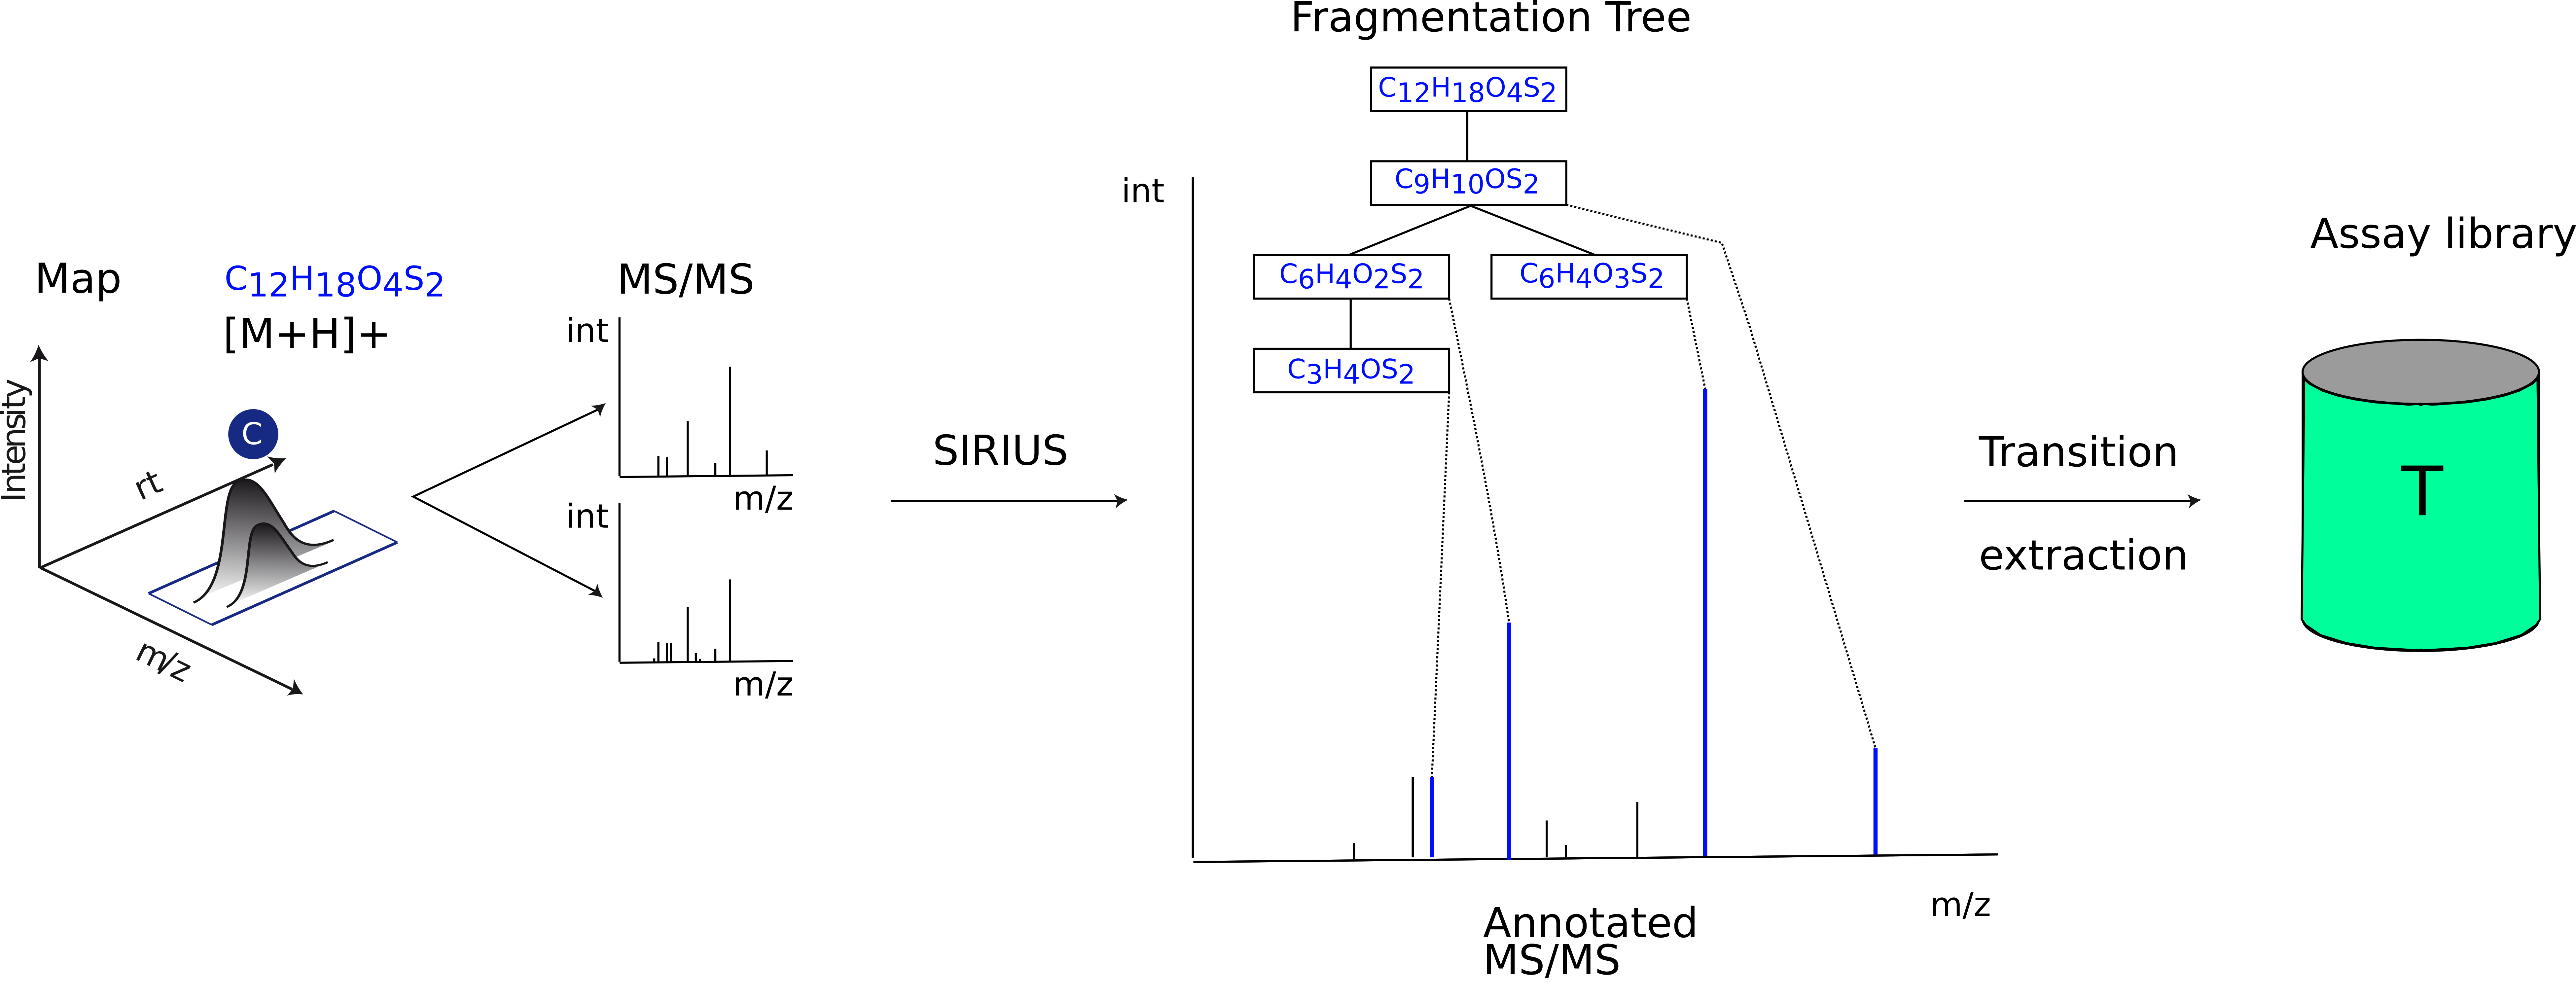
\includegraphics[width=0.8\textwidth]{graphics/openswathmetabo/assay_library_generation.png}
  \caption{\textbf{Assay library generation}  The results of the compound identification (feature, molecular formula, adduct), with the corresponding fragment spectra  for the feature, are used to perform fragment annotation via SIRIUS, using the compositional fragmentation trees. Then, the n highest intensity transitions are extracted and stored in the assay library.}
  \label{fig:assay_library_generation}
\end{figure}

\begin{figure}[!t]
  \centering
  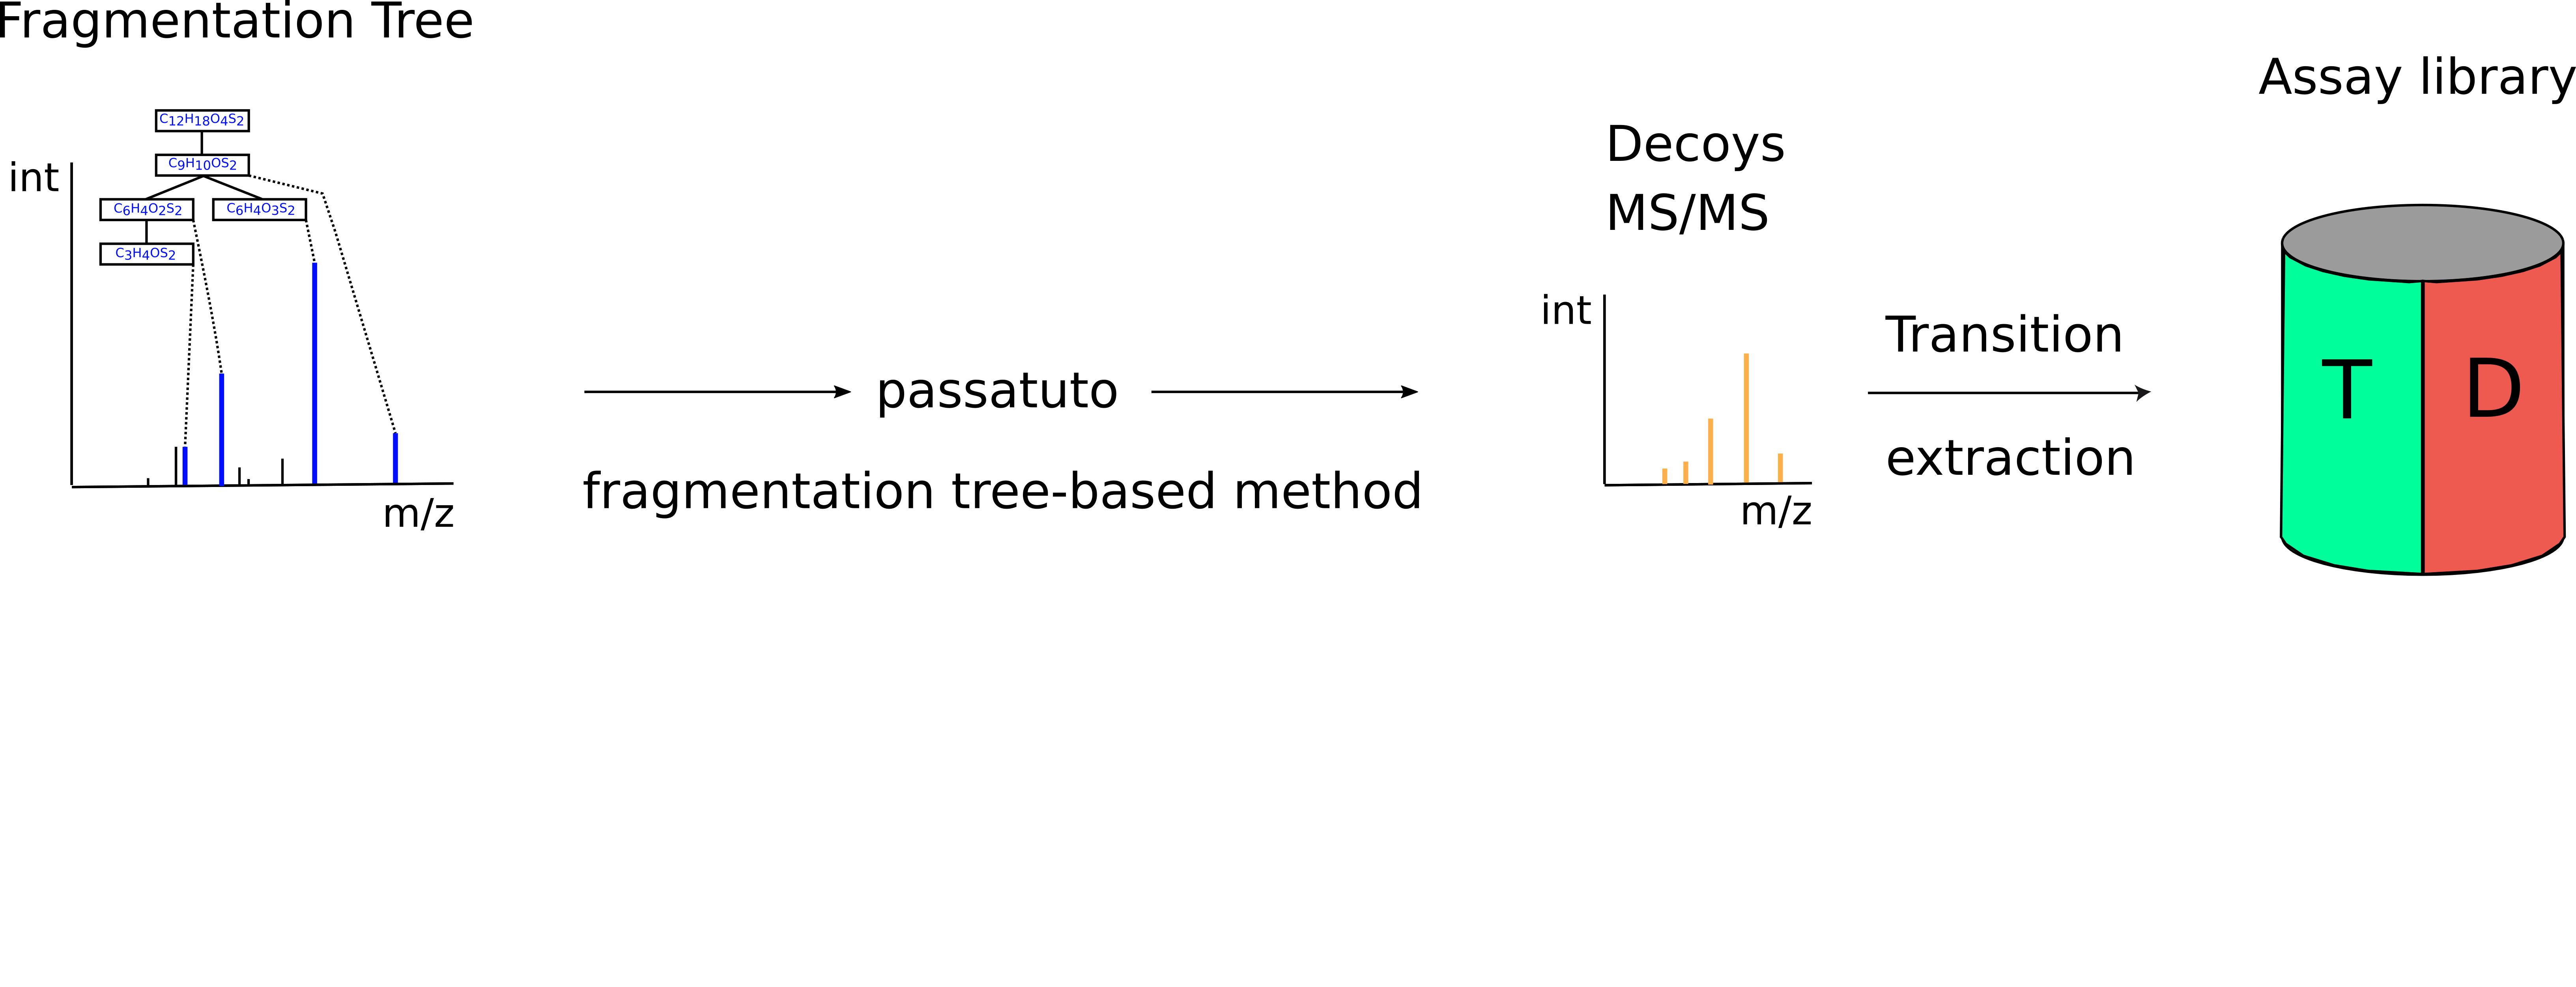
\includegraphics[width=0.8\textwidth]{graphics/openswathmetabo/decoy_generation.png}
  \caption{\textbf{Decoy generation} The compositional fragmentations trees from the step above are used to run the fragmentation tree re-rooting method from Passatutto, generating a compound specific decoy MS2 spectrum. Here, the n highest intensity decoy transitions are extracted and stored in the target-decoy assay library.}
  \label{fig:decoy_generation}
\end{figure}

\subsection{Prerequisites}
Apart from the usual KNIME nodes, the workflow uses python scripting nodes. One basic requirement for the installation of python packages, in particular pyOpenMS, is a package manager for python. Using conda as an environment manger allows to specify a specific environment in the KNIME settings (\menu{File > Preferences > KNIME > Python})

\subsubsection{Windows}
We suggest do use a virtual environment for the Python 3 installation on windows. 
Here you can install miniconda and follow the further instructions. \\

\begin{enumerate}
  \item Create new conda python environment
    \begin{lstlisting}
    	\begin{minted}{bash}
   			conda create -n py39 python=3.9
   		\end{minted}	
    \end{lstlisting} 
  \item Activate py39 environment
    \begin{lstlisting}
    	\begin{minted}{bash}
    		conda activate py39    
    	\end{minted}
    \end{lstlisting} 
  \item Install pip (see above)
  \item On the command line:
    \begin{listing}
\begin{minted}{bash}
    python -m pip install -U pip
    python -m pip install -U numpy
    python -m pip install -U pandas
    python -m pip isntall -U pyprophet
    python -m pip install -U pyopenms
    \end{minted}
\end{listing}
\end{enumerate}

\subsubsection{MacOS}
We suggest do use a virtual environment for the Python 3 installation on Mac. 
Here you can install miniconda and follow the further instructions. \\

\begin{enumerate}
  \item Create new conda python environment
    \begin{lstlisting}
    	\begin{minted}{bash}
    		conda create -n py39 python=3.9
    	\end{minted}
    \end{lstlisting} 
    \item Activate py39 environment
    \begin{lstlisting}
    	\begin{minted}{bash}
    		conda activate py39
    	\end{minted}
    \end{lstlisting} 
  \item On the Terminal:
    \begin{listing}
\begin{minted}{bash}
    python -m pip install -U pip
    python -m pip install -U numpy
    python -m pip install -U pandas
    python -m pip isntall -U pyprophet
    python -m pip install -U pyopenms
    \end{minted}
\end{listing}
\end{enumerate}

\subsubsection{Linux}
Use your package manager apt-get or yum, where possible.
\begin{enumerate}
  \item Install Python 3.9 (Debian: python-dev, RedHat: python-devel)
  \item Install NumPy (Debian / RedHat: python-numpy)
  \item Install setuptools (Debian / RedHat: python-setuptools)
  \item On the Terminal:
    \begin{listing}
\begin{minted}{bash}
    python -m pip install -U pip
    python -m pip install -U numpy
    python -m pip install -U pandas
    python -m pip isntall -U pyprophet
    python -m pip install -U pyopenms
    \end{minted}
\end{listing}
\end{enumerate}

\subsection{Benchmark data}
For the assay library construction pesticide mixes (Agilent Technologies, Waldbronn, Germany) were measured individually in solvent (DDA). 
Benchmark DIA samples were prepared by spiking different commercially available pesticide mixes into human plasma metabolite extracts in a 1:4 dilution series, which covers 5 orders of magnitude.

\noindent The example data can be found here:
\url{https://abibuilder.informatik.uni-tuebingen.de/archive/openms/Tutorials/Data/DIAMetAlyzer/}

\subsection{Example Workflow}
Example workflow for the usage of the DIAMetAlyzer Pipeline in KNIME (see Fig. \ref{fig:oswm_example_wf}). Inputs are the SWATH-MS data in profile mode (.mzML), a path for saving the new target-decoy assay library, the SIRIUS 4.9.0 executable, the DDA data (.mzML), custom libraries and adducts for \KNIMENODE{AccurateMassSearch}, the min/max fragment mass-to-charge to be able to restrict the mass of the transitions and the path to the PyProphet executable. The DDA is used for feature detection, adduct grouping, accurate mass search and forwarded to the \KNIMENODE{AssayGeneratorMetabo}. Here, feature mapping is performed to collect MS2 spectra that belong to a feature. All information collected before (feautre, adduct, putative identification, MS2 spectra) are then internally forwarded to SIRIUS. SIRIUS is used for fragment annotation and decoy generation based on the fragmentation tree re-rooting approach. This information is then used to filter spectra/decoys based on their explained intensity (min. 85\%). Afterwards internal feature linking is performed which is most important for untargeted experiments using a lot of DDA data to construct the library. The constructed target-decoy assay library is processed with the SWATH-MS data in OpenSWATH. The results are used by PyProphet for scoring and output a list of metabolites with their respective q-value and quantitative information.

\begin{figure}[!h]
  \centering
  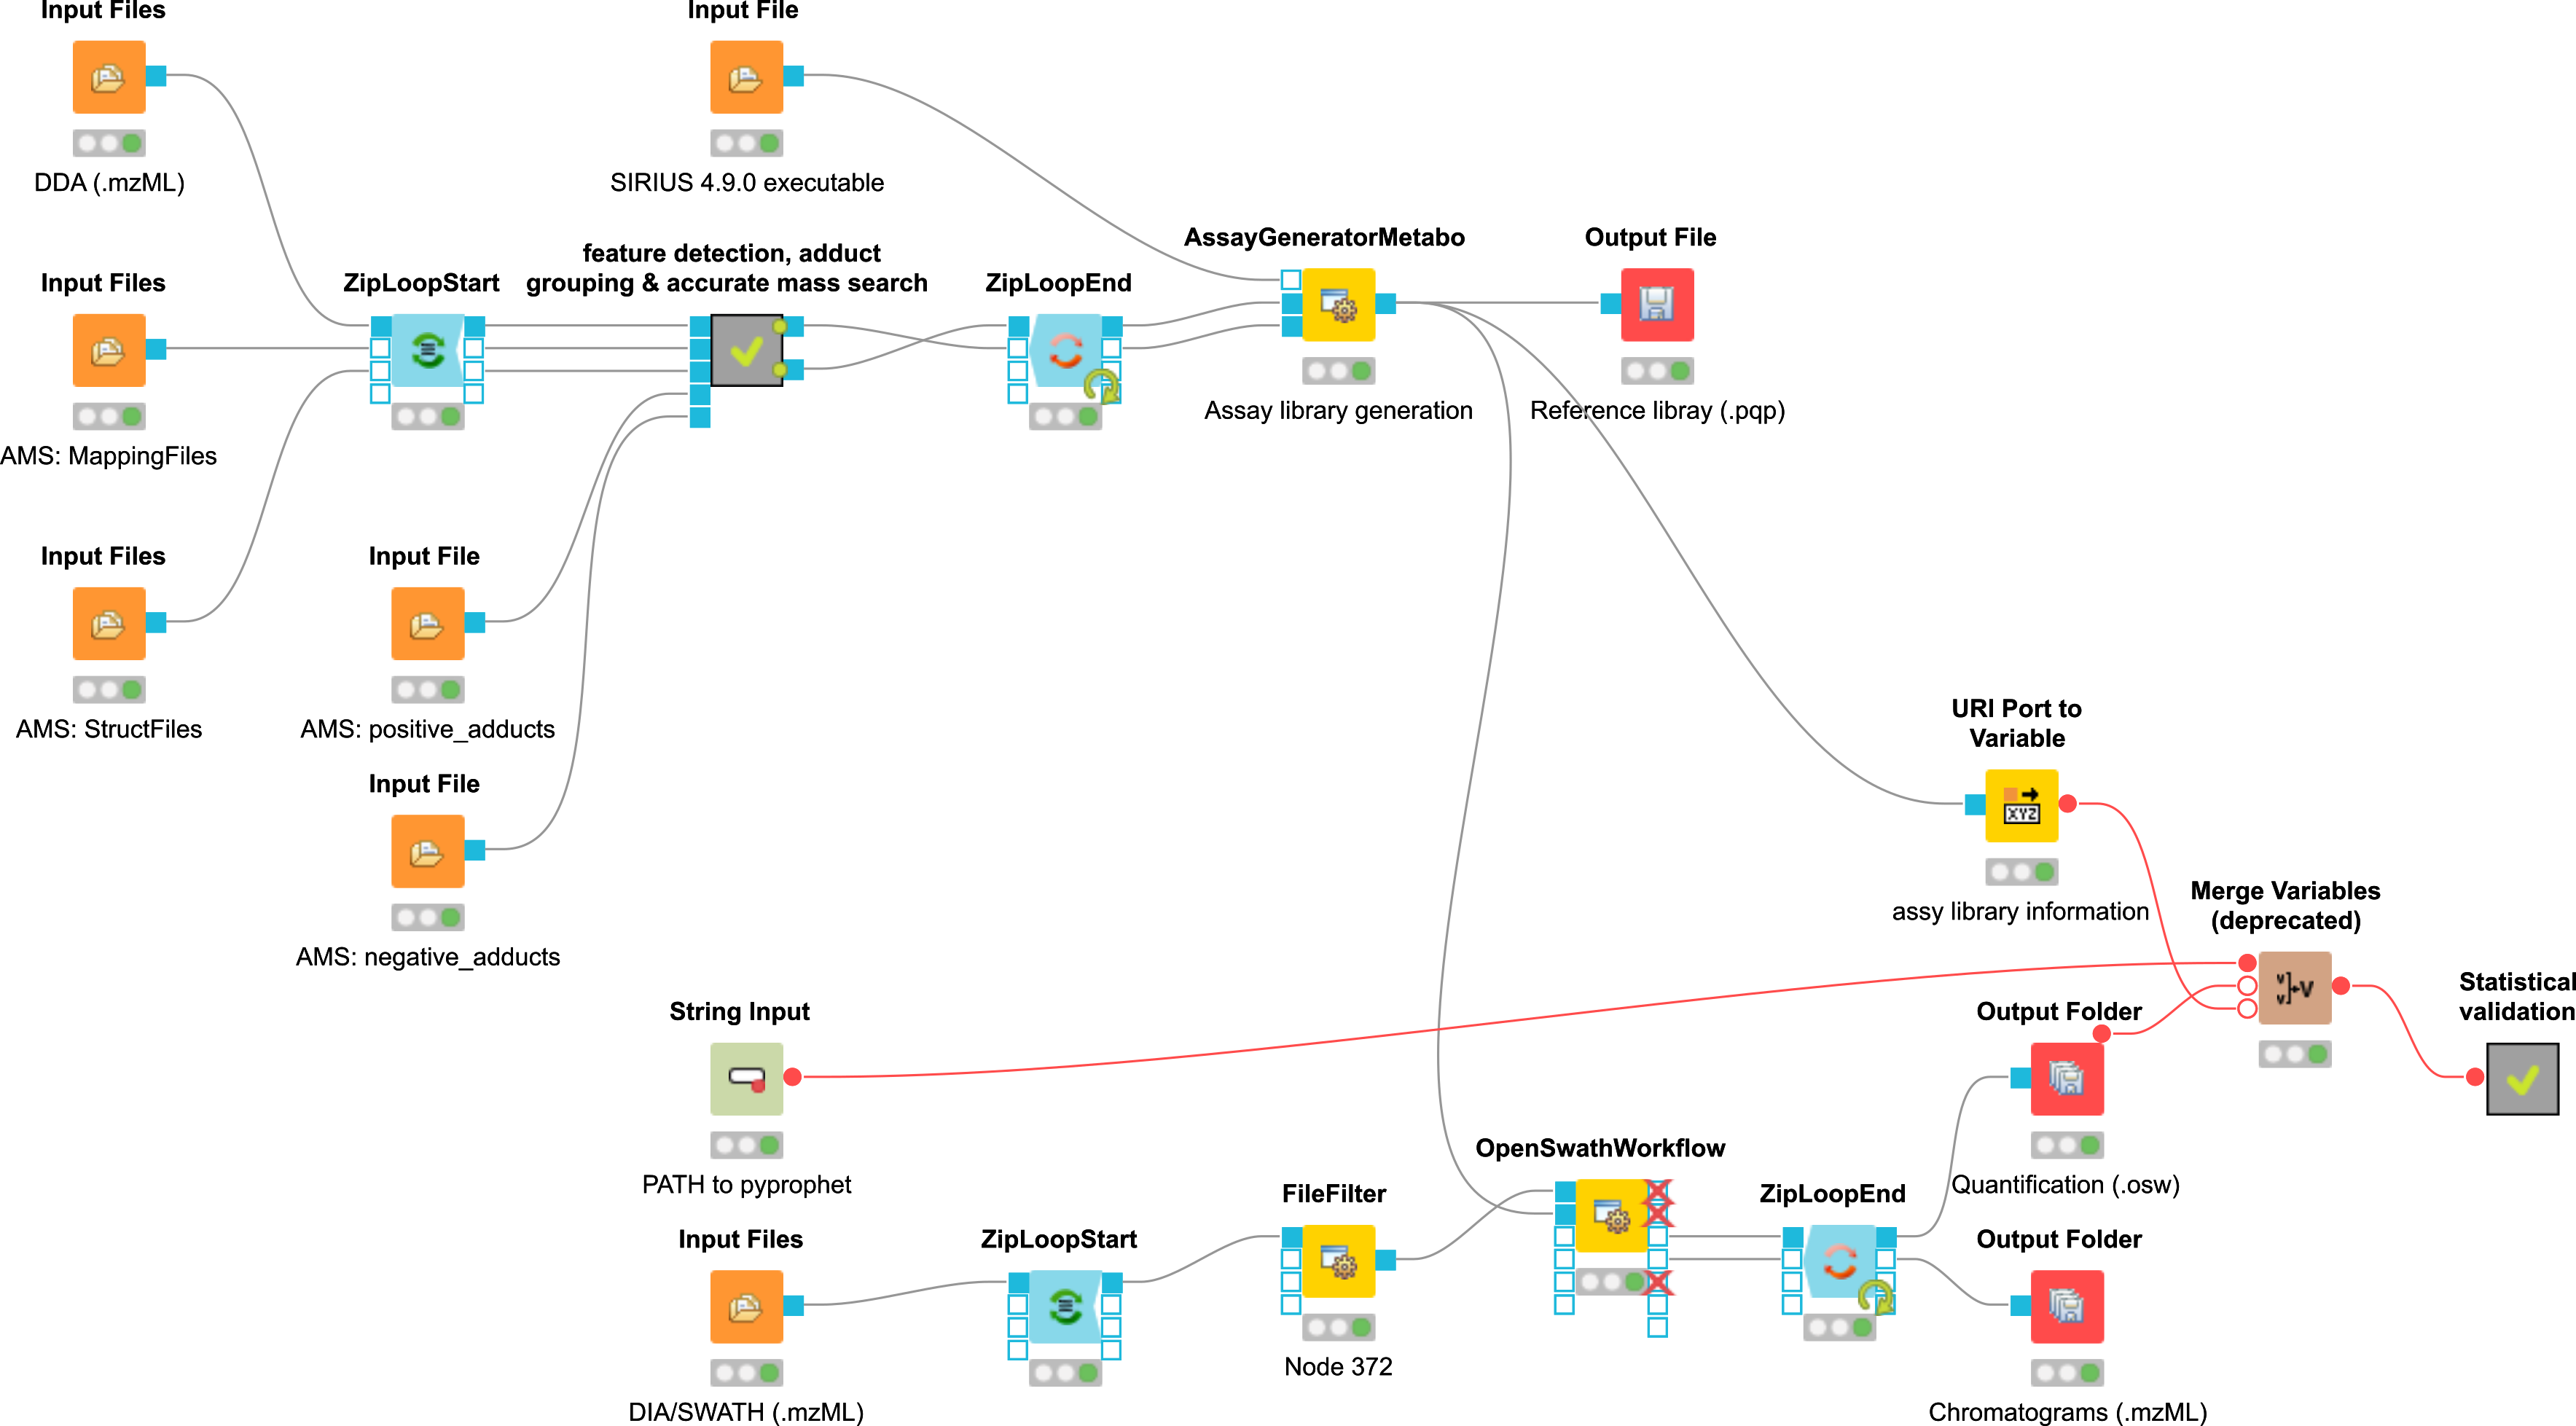
\includegraphics[width=0.95\textwidth]{openswathmetabo/oswm_example_wf.png}
  \caption{Example workflow for the usage of the DIAMetAlyzer Pipeline in KNIME}
  \label{fig:oswm_example_wf}
\end{figure}

\subsection{Run the Workflow}
These steps need to be followed to run the workflow successfully:

\begin{itemize}
\item Add DDA Input Files (.mzML).
\item Specify SIRIUS 4.9.0 executable.
\item Specify library files (mapping, struct) for \KNIMENODE{AccurateMassSearch}.
\item Add positive/negative adducts lists for \KNIMENODE{AccurateMassSearch}
\item Supply an output path for the SIRIUS workspace in the \KNIMENODE{AssayGeneratorMetabo}.
\item Specify additional paths and variables, such as an output path for the target-decoy assay library and a path to the pyprophet installation as well as decoy fragment mz filter (min/max).
\item Input DIA/SWATH files (.mzML).
\item Specify output path in the output folders.
\item Ready to go - run the workflow! 
\end{itemize}

\subsection{Important parameters}
\noindent Please have a look at the most important parameters, which should be tweaked to fit your data. In general, OpenMS has a lot of room for parameter optimization to best fit your chromatography and instrumental settings. \\

\noindent\KNIMENODE{\textbf{FeatureFinderMetabo}}:
\begin{center}
\begin{tabular*}{\textwidth}{ p{5.5cm}|p{10.5cm} }
\textbf{parameter} & \textbf{explanation} \\ \hline
\textit{noise\_threshold\_int} & Intensity threshold below which peaks are regarded as noise. \\
\textit{chrom\_fwhm} & Expected chromatographic peak width (in seconds). \\
\textit{mass\_error\_ppm} & Allowed mass deviation (in ppm) \\
\end{tabular*}
\end{center}

\noindent\KNIMENODE{\textbf{MetaboliteAdductDecharger}}:
\begin{center}
\begin{tabular*}{\textwidth}{ p{5.5cm}|p{10.5cm} }
\textbf{parameter} & \textbf{explanation} \\ \hline
\textit{mass\_max\_diff} & Maximum allowed mass tolerance per feature.. \\
\textit{potential\_adducts} & Adducts used to explain mass differences - These should fit to the adduct list specified for AccurateMassSearch. \\
\end{tabular*}
\end{center}

\noindent\KNIMENODE{\textbf{AccurateMassSearch}}:
\begin{center}
\begin{tabular*}{\textwidth}{ p{5.5cm}|p{10.5cm} }
\textbf{parameter} & \textbf{explanation} \\ \hline
\textit{mass\_error\_value} & Tolerance allowed for accurate mass search. \\
\textit{ionization\_mode} &  Positive or negative ionization mode. \\
\end{tabular*}
\end{center}

\noindent\KNIMENODE{\textbf{AssayGeneratorMetabo}}:
\begin{center}
\begin{tabular*}{\textwidth}{ p{5.5cm}|p{10.5cm} }
\textbf{parameter} & \textbf{explanation} \\ \hline
\textit{min\_transitions} & Minimal number of transitions (3). \\
\textit{max\_transitions} &  Maximal number of transitions (3). \\
\textbf{min\_fragment\_mz} & Minimal m/z of a fragment ion choosen as a transition \\
\textbf{max\_fragment\_mz} & Maximal m/z of a fragment ion choosen as a transition \\
\textit{transitions\_threshold} & Further transitions need at least x\% of the maximum intensity. \\
\textbf{fragment\_annotation\_score\_threshold} & Filters annotations based on the explained intensity of the peaks in a spectrum (0.8). \\
SIRIUS (internal): & \\
\textit{out\_workspace\_directory} & Output directory for SIRIUS workspace (Fragmentation Trees). \\
\textit{filter\_by\_num\_masstraces} &  Features have to have at least x MassTraces. To use this parameter feature\_only is neccessary. \\
\textit{precursor\_mass\_tolerance} & Tolerance window for precursor selection (Feature selection in regard to the precursor). \\
\textit{precursor\_rt\_tolerance} & Tolerance allowed for matching MS2 spectra depeding on the feature size (should be around the FWHM of the chromatograms). \\
\textit{profile} & Specify the used analysis profile (e.g. qtof). \\
\textit{elements} & Allowed elements for assessing the putative sumformula (e.g. CHNOP[5]S[8]Cl[1]). Elements found in the isotopic pattern are added automatically, but can be specified nonetheless. \\
Feature linking (internal): & \\
\textbf{ambiguity\_resolution\_mz\_tolerance} & Mz tolerance for the resolution of identification ambiguity over multiple files - Feature linking m/z tolerance. ) \\
\textbf{ambiguity\_resolution\_rt\_tolerance} & RT tolerance in seconds for the resolution of identification ambiguity over multiple files - Feature linking m/z tolerance. \\
\textbf{total\_occurrence\_filter} & Filter compound based on total occurrence in analysed samples.\\
\end{tabular*}
\end{center}

In case of the \textbf{total\_occurrence\_filter} the value to chose depends on the analysis strategy used. In the instance you are using only identified compounds (\textbf{use\_known\_unkowns} = false) - it will filter based on identified features. This means that even if the feature was detected in e.g. 50\% of all samples it might be only identified correctly by accurate mass search in 20\% of all samples. Using a \textbf{total\_occurrence\_filter} this specific feature would still be filtered out  due to less identifications. 

\noindent\KNIMENODE{\textbf{OpenSWATH}}:
\begin{center}
\begin{tabular*}{\textwidth}{ p{5.5cm}|p{10.5cm} }
\textbf{parameter} & \textbf{explanation} \\ \hline
\textit{rt\_extraction\_window} & Extract x seconds around this value. \\
\textit{rt\_normalization\_factor} &  Please use the range of your gradient e.g. 950 seconds. \\
\end{tabular*}
\end{center} 

\noindent If you are analysing a lot of big DIA mzML files $\approx$ 3-20GB per File, it makes sense to change how OpenSWATH processes the spectra. 

\begin{center}
\begin{tabular*}{\textwidth}{ p{5.5cm}|p{10.5cm} }
\textbf{parameter} & \textbf{explanation} \\ \hline
\textit{readOptions} & Set cacheWorkingInMemory - will cache the files to disk and read SWATH-by-SWATH into memory\\
\textit{tempDirectory} &  Set a directory, where cached mzMLs are stored (be aware that his directory can be quite huge depending on the data). \\
\end{tabular*}
\end{center} 

\noindent In the workflow pyprophet is called after OpenSWATH, it merges the result files, which allows to get enough data for the model training. 

\begin{listing}
\begin{minted}{bash}
pyprophet merge  --template path_to_target-decoy_assay_library.pqp --out merged.osw  ./*.osw
\end{minted}
\end{listing}

\noindent Afterwards, the results are scored using the MS1 and MS2 levels and filter for metabolomics scores, which have a low correlation. 

\begin{listing}
\begin{minted}{bash}
pyprophet score --in  merged.osw  --out  scored.osw --level ms1ms2 --ss_main_score "var_isotope_correlation_score" --ss_score_filter metabolomics
\end{minted}
\end{listing}
\noindent Export the non filtered results: 

\begin{listing}
\begin{minted}{bash}
pyprophet export-compound --in scored.osw --out scored + "_pyprophet_nofilter_ms1ms2.tsv" 
--max_rs_peakgroup_qvalue 1000.0
\end{minted}
\end{listing}
\noindent Please see the workflow for actual parameter values used for the benchmarking dataset. \\

\noindent  The workflow can be used without any identification (remove \KNIMENODE{AccurateMassSearch}). Here, all features (known\_unknowns) are processed. The assay library is constructed based on the chemical composition elucidated via the fragment annotation (SIRIUS 4). It is also possible to use identified and in addition unknown (non-identified) features, by using \KNIMENODE{AccurateMassSearch} in combination with the \textbf{use\_known\_unknowns} in the \KNIMENODE{AssayGeneratorMetabo}.  


%!TEX root = handout.tex

\newpage
\section{An introduction to pyOpenMS}

\subsection{Introduction}
pyOpenMS provides Python bindings for a large part of the OpenMS library for mass spectrometry based proteomics and metabolomics. It thus provides access to a feature-rich, open-source algorithm library for mass-spectrometry based LC-MS analysis. These Python bindings allow raw access to the data-structures and algorithms implemented in {OpenMS, specifically those for file access (mzXML, mzML, TraML, mzIdentML among others), basic signal processing (smoothing, filtering, de-isotoping and peak-picking) and complex data analysis (including label-free, SILAC, iTRAQ and SWATH analysis tools).\\

\noindent pyOpenMS is integrated into OpenMS starting from version 1.11. This tutorial is addressed to people already familiar with Python. If you are new to Python, we suggest to start with a Python tutorial (\url{https://en.wikibooks.org/wiki/Non-Programmer%27s_Tutorial_for_Python_3}).

\subsection{Installation}
One basic requirement for the installation of python packages, in particular pyOpenMS, is a package manager for python. We provide a package for \textit{pip} (\url{https://pypi.python.org/pypi/pip}).

\subsubsection{Windows}
\begin{enumerate}
  \item Install Python 3.7 (\url{http://www.python.org/download/})
  \item Install NumPy (\url{http://www.lfd.uci.edu/~gohlke/pythonlibs/#numpy})
  \item Install pip (see above)
  \item On the command line:
    \begin{listing}
\begin{minted}{bash}
    python -m pip install -U pip
    python -m pip install -U numpy
    python -m pip install pyopenms
    \end{minted}
\end{listing}
\end{enumerate}

\subsubsection{MacOS}
We suggest do use a virtual environment for the Python 3 installation on Mac. 
Here you can install miniconda and follow the further instructions. \\

\begin{enumerate}
  \item Create new conda python environment
    \begin{listing}
\begin{minted}{bash}
    conda create -n py37 python=3.7 anaconda
    \end{minted}
\end{listing} 
    \item Activate py37 environment
    \begin{listing}
\begin{minted}{bash}
    source activate py37
    \end{minted}
\end{listing} 
  \item On the Terminal:
    \begin{listing}
\begin{minted}{bash}
    pip install -U pip
    pip install -U numpy
    pip install pyopenms
    \end{minted}
\end{listing}
\end{enumerate}

\subsubsection{Linux}
Use your package manager apt-get or yum, where possible.
\begin{enumerate}
  \item Install Python 3.7 (Debian: python-dev, RedHat: python-devel)
  \item Install NumPy (Debian / RedHat: python-numpy)
  \item Install setuptools (Debian / RedHat: python-setuptools)
  \item On the Terminal:
    \begin{listing}
\begin{minted}{bash}
    pip install pyopenms
    \end{minted}
\end{listing}
\end{enumerate}

\subsubsection{IDE with Anaconda integration}
If you do not have python installed or do not want to modify your native installation, another possibility is to use an IDE (integrated development environment) with Anaconda integration. Here, we recommend spyder (\url{https://www.spyder-ide.org/}). It comes with Anaconda, which is a package and environment manager. Thus the IDE should be able to run a specific environment independent of your systems python installation. \\

\noindent Please execute the installer for your respective platform located in the respective directory for your platform and follow the installation instructions. \\

\noindent After installation the ANACONDA Navigator (Anaconda 3) should be available. Please start the application. To install pyopenms please choose the button "Environments" and click the play symbol of the base environment and "Open Terminal". \\

\noindent  Update pip and install pyopenms (MacOS, Linux):
\begin{listing}
\begin{minted}{bash}
pip install -U pip
pip install -U numpy
pip install -U pyopenms
\end{minted}
\end{listing}

\noindent  Update pip and install pyopenms (Windows):
\begin{listing}
\begin{minted}{bash}
python -m pip install -U pip
python -m pip install -U numpy
python -m pip install -U pyopenms
\end{minted}
\end{listing}

\noindent Install a local available package:
\begin{listing}
\begin{minted}{bash}
pip install numpy-1.15.4-cp37*.whl
pip install pyopenms-2.4.0-cp37*.whl
or (in case of windows)
python -m pip install -U numpy-1.15.4-cp37*.whl
python -m pip install -U pyopenms-2.4.0-cp37*.whl
\end{minted}
\end{listing}

\noindent The local available packages can be found in the directory corresponding to your operating system. Please use the absolute path to the packages for the installation.
    
\noindent  Now launch "Spyder" (python IDE) in the home menu.

\subsection{Build instructions}
Instructions on how to build pyOpenMS can be found online (\url{https://pyopenms.readthedocs.io/en/release_2.4.0/build_from_source.html}).

\subsection{Scripting with pyOpenMS}
A big advantage of pyOpenMS are its scripting capabilities (beyond its application in tool development). Most of the OpenMS datastructure can be accessed using python (\url{https://abibuilder.informatik.uni-tuebingen.de/archive/openms/Documentation/nightly/html/index.html}). Here we would like to give some examples on how pyOpenMS can be used for simple scripting task, such as peptide mass calculation and peptide/protein digestion as well as isotope distribution calculation. \\

\noindent Calculation of the monoisotopic and average mass of a peptide sequence 
\begin{listing}
\begin{minted}{python}
from pyopenms import *

seq = AASequence.fromString("DFPIANGER")

mono_mass = seq.getMonoWeight(Residue.ResidueType.Full, 0)
average_mass = seq.getAverageWeight(Residue.ResidueType.Full, 0)

print("The masses of the peptide sequence " + seq.toString().decode('utf-8') + " are:")
print("mono: " + str(mono_mass))
print("average: "+ str(average_mass))
\end{minted}
\end{listing}

\noindent Enzymatic digest of a peptide/protein sequence 
\begin{listing}
\begin{minted}{python}
enzyme = "Trypsin"
to_digest = AASequence.fromString("MKWVTFISLLLLFSSAYSRGVFRRDTHKSEIAHRFKDLGE")
after_digest = []

EnzymaticDigest = EnzymaticDigestionLogModel()
EnzymaticDigest.setEnzyme(enzyme)
EnzymaticDigest.digest(to_digest, after_digest)

print("The peptide " + to_digest.toString().decode('utf-8') + " was digested using " + str(EnzymaticDigest.getEnzymeName().decode('utf-8')) + " to:")

for element in after_digest:
    print(element.toString().decode('utf-8'))
\end{minted}
\end{listing}

\noindent Use empirical formula to calculate the isotope distribution 
\begin{listing}
\begin{minted}{python}
from pyopenms import *

methanol = EmpiricalFormula("CH3OH")
water = EmpiricalFormula("H2O")
wm = EmpiricalFormula(water.toString().decode('utf-8') + methanol.toString().decode('utf-8'))
print(wm.toString().decode('utf-8'))
print(wm.getElementalComposition())

isotopes = wm.getIsotopeDistribution( CoarseIsotopePatternGenerator(3) )
for iso in isotopes.getContainer():
    print (iso.getMZ(), ":", iso.getIntensity())
\end{minted}
\end{listing}

\noindent For further examples and the pyOpenMS datastructure please see \url{https://pyopenms.readthedocs.io/en/release_2.4.0/datastructures.html}. 

\subsection{Tool development with pyOpenMS}
Scripting is one side of pyOpenMS, the other is the ability to create Tools using the C++ OpenMS library in the background.  In the following section we will create a "ProteinDigestor" pyOpenMS Tool. It should be able to read in a fasta file. Digest the proteins with a specific enzyme (e.g. Trypsin) and export an idXML output file. Please see  \directory{Example\_Data/pyopenms} for code snippets.

\begin{listing}
\begin{minted}{bash}
usage: ProteinDigestor.py [-h] [-in INFILE] [-out OUTFILE] [-enzyme ENZYME]
                          [-min_length MIN_LENGTH] [-max_length MAX_LENGTH]
                          [-missed_cleavages MISSED_CLEAVAGES]

ProteinDigestor −− In silico digestion of proteins.

optional arguments:
  -h, --help            show this help message and exit
  -in INFILE            An input file containing amino acid sequences [fasta]
  -out OUTFILE          Output digested sequences in idXML format [idXML]
  -enzyme ENZYME        Enzyme used for digestion
  -min_length MIN_LENGTH		Minimum length of peptide
  -max_length MAX_LENGTH		Maximum length of peptide
  -missed_cleavages MISSED_CLEAVAGES			The number of allowed missed cleavages
\end{minted}
\end{listing}

\subsubsection{Basics}
First, your tool needs to be able to read parameters from the command line and provide a main routine. Here standard Python can be used (no pyOpenMS is required so far).

\begin{listing}
\begin{minted}{python}
#!/usr/bin/env python
import sys

def main(options):

    # test parameter handling
    print(options.infile, options.outfile, options.enzyme, options.min_length, options.max_length, options.missed_cleavages)

def handle_args():
    import argparse

    usage = ""
    usage += "\nProteinDigestor −− In silico digestion of proteins."

    parser = argparse.ArgumentParser(description = usage)
    parser.add_argument('-in', dest='infile', help='An input file containing amino acid sequences [fasta]')
    parser.add_argument('-out', dest='outfile', help='Output digested sequences in idXML format [idXML]')
    parser.add_argument('-enzyme', dest='enzyme', help='Enzyme used for digestion')
    parser.add_argument('-min_length', type=int, dest='min_length', help ='Minimum length of peptide')
    parser.add_argument('-max_length', type=int, dest='max_length', help='Maximum length of peptide')
    parser.add_argument('-missed_cleavages', type=int, dest='missed_cleavages', help='The number of allowed missed cleavages')

    args = parser.parse_args(sys.argv[1:])
    return args

if __name__ == '__main__':
    options = handle_args()
    main(options)
\end{minted}
\end{listing}

\noindent Open the Anaconda Terminal and change into the \directory{Example\_Data/pyopenms} directory. Execute the example script. 
\begin{listing}
\begin{minted}{bash}
python ProteinDigestor_argparse.py -h
\end{minted}
\end{listing}

\begin{listing}
\begin{minted}{bash}
python ProteinDigestor_argparse.py -in mini_example.fasta -out mini_example_out.idXML -enzyme Trypsin -min_length 6 -max_length 40 -missed_cleavages 1
\end{minted}
\end{listing}

\noindent The parameters are being read from the command line by the function handle\_args() and given to the main() function of the script, which prints the different variables.

\noindent OpenMS has a ProteaseDB  class containing a list of enzymes which can be used for digestion of proteins. You can add this to the argparse code to be able to see the usable enzymes. From this point onward pyOpenMS is required. 
\begin{listing}
\begin{minted}{python}
    # from here pyopenms is needed
    # get available enzymes from ProteaseDB
    all_enzymes = []
    p_db=ProteaseDB().getAllNames(all_enzymes)
    
    # concatenate them to the enzyme argument.
    parser.add_argument('-enzyme', dest='enzyme', help='Enzymes which can be used for digestion: '+ ', '.join(map(bytes.decode, all_enzymes)))
\end{minted}
\end{listing}

\subsubsection{Loading data structures with pyOpenMS}
We already scripted enzymatic digestion with the AASequence and EnzymaticDigest (see above). To make this even easier, we can use an existing class in OpenMS, called ProteaseDigestion.

\begin{listing}
\begin{minted}{python}
    # Use the ProteaseDigestion class
    # set the enzyme used for digestion and the number of missed cleavages
    digestor = ProteaseDigestion()
    digestor.setEnzyme(options.enzyme)
    digestor.setMissedCleavages(options.missed_cleavages)
    
    # call the ProteaseDigestion::digest function
    # which will return the number of discarded digestions products  
    # and fill the current_digest list with digestes peptide sequences
    digestor.digest(aaseq.fromString(fe.sequence), current_digest, options.min_length, options.max_length)
\end{minted}
\end{listing}

\noindent The next step is to use FASTAFile class to read the fasta input:
\begin{listing}
\begin{minted}{python}
    # construct a FASTAFile Object and read the input file
    ff = FASTAFile()
    ff.readStart(options.infile)
    
    # construct and FASTAEntry Object 
    fe = FASTAEntry()
    
    # loop over the entry in the fasta while using while
    while(ff.readNext(fe)): 
\end{minted}
\end{listing}

\noindent The output idXML needs the information about protein and peptide level, which can be saved in the ProteinIdentification and PeptideIdentification classes. 
\begin{listing}
\begin{minted}{python}
    idxml = IdXMLFile()
    idxml.store(options.outfile, protein_identifications, peptide_identifications)
\end{minted}
\end{listing}

\noindent This is the part of the program which unifies the snippets provided above. Please have a closer look how the protein and peptide datastructure is incorporated in the program. 

\begin{listing}
\begin{minted}{python}
def main(options):
    # read fasta file  
    ff = FASTAFile()
    ff.readStart(options.infile)
    fe = FASTAEntry()

    # use ProteaseDigestion class 
    digestor = ProteaseDigestion()
    digestor.setEnzyme(options.enzyme)
    digestor.setMissedCleavages(options.missed_cleavages)

    # protein and peptide datastructure
    protein_identifications = []
    peptide_identifications = []
    protein_identification = ProteinIdentification()
    protein_identifications.append(protein_identification)
    temp_pe = PeptideEvidence()

    # number of dropped peptides due to length restriction
    dropped_by_length = 0

    while(ff.readNext(fe)):  
        # construct ProteinHit and fill it with sequence information
        temp_protein_hit = ProteinHit()
        temp_protein_hit.setSequence(fe.sequence)
        temp_protein_hit.setAccession(fe.identifier)

        # save the ProteinHit in a ProteinIdentification Object 
        protein_identification.insertHit(temp_protein_hit)
       
        # construct a PeptideHit and save the ProteinEvidence (Mapping) for the specific 
        # current protein
        temp_peptide_hit = PeptideHit()
        temp_pe.setProteinAccession(fe.identifier);
        temp_peptide_hit.setPeptideEvidences([temp_pe])

        # digestion 
        current_digest = []
        aaseq = AASequence()
        if (options.enzyme == "none"):
            current_digest.append(aaseq.fromString(fe.sequence))
        else:
            dropped_by_length += digestor.digest(aaseq.fromString(fe.sequence), current_digest, options.min_length, options.max_length)

        for seq in current_digest:
            # fill the PeptideHit and PeptideIdentification datastructure
            peptide_identification = PeptideIdentification() 
            temp_peptide_hit.setSequence(seq)
            peptide_identification.insertHit(temp_peptide_hit)
            peptide_identifications.append(peptide_identification)

    print(str(dropped_by_length) + " peptides have been dropped due to the length restriction.")
    idxml = IdXMLFile()
    idxml.store(options.outfile, protein_identifications, peptide_identifications)
\end{minted}
\end{listing}

\subsubsection{Putting things together}
The paramter input and the functions can be used to construct the program we are looking for. If you are struggling please have a look in the example data section ProteinDigestor.py 

\noindent Now you can run your tool in the Anaconda Terminal ( \directory{Example\_Data/pyopenms}): 
\begin{listing}
\begin{minted}{bash}
python ProteinDigestor.py -in mini_example.fasta -out mini_example_out.idXML -enzyme Trypsin -min_length 6 -max_length 40 -missed_cleavages 1
\end{minted}
\end{listing}

\subsubsection{Bonus task}

\begin{task}
Implement all other 184 TOPP tools using pyOpenMS.
\end{task}


%!TEX root = handout.tex

\newpage
\section{Quality control}
\label{sec:qc}

\subsection{Introduction}

In this chapter, we will build on an existing workflow with OpenMS / KNIME to add some quality control (QC). We will utilize the qcML tools in OpenMS to create a file with which we can collect different measures of quality to the mass spectrometry runs themselves and the applied analysis. The file also serves the means of visually reporting on the collected quality measures and later storage along the other analysis result files.
We will, step-by-step, extend the label-free quantitation workflow from section \ref{sec:lfq} with QC functions and thereby enrich each time the report given by the qcML file.
But first, to make sure you get the most of this tutorial section, a little primer on how we handle QC on the technical level. \\

\subsubsection*{QC metrics and qcML}
To assert the quality of a measurement or analysis we use quality metrics. Metrics are describing a certain aspect of the measurement or analysis and can be anything from a single value, over a range of values to an image plot or other summary. Thus, qcML metric representation is divided into QC parameters (QP) and QC attachments (QA) to be able to represent all sorts of metrics on a technical level.\\
A QP may (or may not) have a value which would equal a metric describable with a single value. If the metric is more complex and needs more than just a single value, the QP does not require the single value but rather depends on an attachment of values (QA) for full meaning. Such a QA holds the plot or the range of values in a table-like form. Like this, we can describe any metric by a QP and an optional QA.\\
To assure a consensual meaning of the quality parameters and attachments, we created a controlled vocabulary (CV). Each entry in the CV describes a metric or part/extension thereof. We embed each parameter or attachment with one of these and by doing so, connect a meaning to the QP/QA. Like this, we later know exactly what we collected and the programs can find and connect the right dots for rendering the report or calculating new metrics automatically. You can find the constantly growing controlled vocabulary here:\\ \menu{https://github.com/qcML/qcML-development/blob/master/cv/qc-cv.obo}.\\
Finally, in a qcml file, we split the metrics on a per mass-spectrometry-run base or a set of mass-spectrometry-runs respectively. Each run or set will contain its QP/QA we calculate for it, describing their quality.


\subsection{Building a qcML file per run}
\label{Building a qcML file per run}

As a start, we will build a basic qcML file for each mzML file in the label-free analysis. We are already creating the two necessary analysis files to build a basic qcML file upon each mzML file, a feature file and an identification file. We use the \KNIMENODE{QCCalculator} node from \menu{Community Nodes > OpenMS > Utilities} where also all other \KNIMENODE{QC*} nodes will be found. The \KNIMENODE{QCCalculator} will create a very basic qcML file in which it will store collected and calculated quality data.

\begin{itemize} 
\item Copy your label-fee quantitation workflow into a new lfq-qc workflow and open it.
\item Place the \KNIMENODE{QCCalculator} node after the \KNIMENODE{IDMapper} node. Being inside the \KNIMENODE{ZipLoop}, it will execute for each of the three mzML files the \KNIMENODE{Input} node.
\item Connect the first \KNIMENODE{QCCalculator} port to the first \KNIMENODE{ZipLoopStart} outlet port, which will carry the individual mzML files.
\item Connect the last's \KNIMENODE{ID} outlet port (\KNIMENODE{IDFilter} or the \KNIMENODE{ID} metanode) to the second \KNIMENODE{QCCalculator} port for the identification file.
\item Finally, connect the \KNIMENODE{IDMapper} outlet to the third \KNIMENODE{QCCalculator} port for the feature file.
\end{itemize}

The created qcML files will not have much to show for, basic as they are. So we will extend them with some basic plots.
\begin{itemize}
\item First, we will add an 2D overview image of the given mass spectrometry run as you may know it from \OPENMSTOOL{TOPPView}. Add the \KNIMENODE{ImageCreator} node from \menu{Community Nodes > OpenMS > Utilities}. Change the \textit{width} and \textit{heigth} parameters to 640x640 as we don't want it to be too big. Connect it to the first \KNIMENODE{ZipLoopStart} outlet port, so it will create an image file of the mzML's contained run.
\item Now we have to embed this file into the qcML file, and attach it to the right QualityParameter. For this, place a \KNIMENODE{QCEmbedder} node behind the \KNIMENODE{ImageCreator} and connect that to its third inlet port. Connect its first inlet port to the outlet of the \KNIMENODE{QCCalculator} node to pass on the qcML file. Now change the parameter \textit{cv\_acc} to \textit{QC:0000055} which designates the attached image to be of type  \texttt{QC:0000055 - MS experiment heatmap}.
Finally, change the parameter \textit{qp\_att\_acc} to \textit{QC:0000004}, to attach the image to the QualityParameter \texttt{QC:0000004 - MS acquisition result details}.
\item For a reference of which CVs are already defined for qcML, have a look at \\ \menu{https://github.com/qcML/qcML-development/blob/master/cv/qc-cv.obo}.
\end{itemize}

There are two other basic plots which we almost always might want to look at before judging the quality of a mass spectrometry run and its identifications: the \textit{total ion current} (TIC) and the \textit{PSM mass error} (Mass accuracy), which we have available as pre-packaged QC metanodes.
\begin{task}
Import the workflow from \directory{Workflows / Quality Control / QC Metanodes.zip} in KNIME: \menu{File > Import KNIME Workflow...}
\end{task}
\begin{itemize}
\item Copy the \KNIMENODE{Mass accuracy} metanode into the workflow behind the \KNIMENODE{QCEmbedder} node and connect it. The qcML will be passed on and the Mass accuracy plots added. The information needed was already collected by the \KNIMENODE{QCCalculator}.
\item Do the same with the \KNIMENODE{TIC} metanode so that your qcML file will get passed on and enriched on each step. 
\end{itemize}

R Dependencies: This section requires that the R packages ggplot2 and scales are both installed. This is the same procedure as in section \ref{sec:metaboR}. In case that you use an R installation where one or both of them are not yet installed, open the \KNIMENODE{R Snippet} nodes inside the metanodes you just used (double-click). Edit the script in the \textit{R Script} text editor from:\\

\begin{listing}
\begin{minted}{R}
#install.packages("ggplot2")
#install.packages("scales")
\end{minted}
\end{listing}
to 
\begin{listing}
\begin{minted}{R}
install.packages("ggplot2")
install.packages("scales")
\end{minted}
\end{listing}
Press \menu{Eval script} to execute the script.\newline

\vspace{1cm}

\begin{figure}[htbp]
  \centering
  \includegraphics[width=0.85\textwidth]{graphics/qc/qc_basic}
  \caption{Basic QC setup within a LFQ workflow}
  \label{fig:qc_basic}
\end{figure}

\note{To have a peek into what our qcML now looks like for one of the \KNIMENODE{ZipLoop} iterations, we can add an \KNIMENODE{Output Folder} node from \menu{Community Nodes > GenericKnimeNodes > IO} and set its destination parameter to somewhere we want to find our intermediate qcML files in, for example \menu{tmp > qc\_lfq}. If we now connect the last metanode with the \KNIMENODE{Output Folder} and restart the workflow, we can start inspecting the qcML files. }
\begin{task}
Find your first created qcML file and open it with the browser (not IE), and the contained QC parameters will be rendered for you.
\end{task}


\subsection{Adding brand new QC metrics}
\label{Adding brand new QC metrics}

We can also add brand new QC metrics to our qcML files. Remember the \KNIMENODE{Histogram} you added inside the \KNIMENODE{ZipLoop} during the label-free quantitation section? %TODO reference
 Let's imagine for a moment this was a brand new and utterly important metric and plot for the assessment of your analyses quality. There is an easy way to integrate such new metrics into your qcMLs. Though the \KNIMENODE{Histogram} node cannot pass its plot to an \textit{image}, we can do so with a \KNIMENODE{R View (table)}. 

\begin{itemize}
\item Add an \KNIMENODE{R View (table)} next to the \KNIMENODE{IDTextReader} node and connect them.
\item Edit the \KNIMENODE{R View (table)} by adding the \textit{R Script} according to this:
\end{itemize}
\begin{listing}
\begin{minted}{R}
#install.packages("ggplot2")
library("ggplot2")
ggplot(knime.in, aes(x=peptide_charge)) + 
 geom_histogram(binwidth=1, origin =-0.5) + 
 scale_x_discrete() + 
 ggtitle("Identified peptides charge histogram") + 
 ylab("Count")
\end{minted}
\end{listing}
\begin{itemize}
\item This will create a plot like the \KNIMENODE{Histogram} node on \textit{peptide\_charge} \textbf{and} pass it on as an \textit{image}. 
\item Now add and connect a \KNIMENODE{Image2FilePort} node from \menu{Community Nodes > GenericKnimeNodes > Flow} to the \KNIMENODE{R View (table)}.
\item We can now use a \KNIMENODE{QCEmbedder} node like before to add our new metric plot into the qcML.
\item After looking for an appropriate target in \\ \menu{https://github.com/qcML/qcML-development/blob/master/cv/qc-cv.obo}, we found that we can attach our plot to the \textit{MS identification result details} by setting the parameter \textit{qp\_att\_acc} to \textit{QC:0000025}, as we are plotting the charge histogram of our \textit{identified} peptides.
\item To have the plot later displayed properly, we assign it the parameter \textit{cv\_acc} of \textit{QC:0000051}, a \textit{generic plot}. Also we made sure in the \textit{R Script}, that our plot carries a caption so that we know which is which, if we had more than one new plot.
\item Now we redirect the \KNIMENODE{QCEmbedder}s output to the \KNIMENODE{Output Folder} from before and can have a look at how our qcML is coming along after restarting the workflow.
\end{itemize}

\begin{figure}[htbp]
  \centering
  \includegraphics[width=0.65\textwidth]{graphics/qc/qc_extra}
  \caption{QC with new metric}
  \label{fig:qc_extra}
\end{figure}

\newpage
\subsection{Set QC metrics}
\label{Set QC metrics}

Besides monitoring the quality of each individual mass spectrometry run analysis, another capability of QC with OpenMS and qcML is to monitor the complete set. The easiest control is to compare mass spectrometry runs which should be similar, e.g. technical replicates, to spot any aberrations in the set.\\
For this, we will first collect all created qcML files, merge them together and use the qcML onboard \textit{set QC} properties to detect any outliers.

\begin{itemize}
\item connect the \KNIMENODE{QCEmbedder}s output from last section to the \KNIMENODE{ZipLoopEnd}s second input port. 
\item The corresponding output port will collect all qcML files from each \KNIMENODE{ZipLoop} iteration and pass them on as a list of files.
\item Now we add a \KNIMENODE{QCMerger} node after the \KNIMENODE{ZipLoopEnd} and feed it that list of qcML files. In addition, we set its parameter \textit{setname} to give our newly created set a name - say \textit{spikein\_replicates}.
\item To inspect all the QCs next to each other in that created qcML file, we have to add a new \KNIMENODE{Output Folder} to which we can connect the \KNIMENODE{QCMerger} output.
\end{itemize}

When inspecting the set-qcML file in a \textbf{browser}, we will be presented another overview. After the set content listing, the basic QC parameters (like number of identifications) are each displayed in a graph. Each set member (or run) has its own section on the x-axis and each run is connected with that graph via a link in the mouseover on one of the QC parameter values.

\newpage

\begin{figure}[htbp]
  \centering
  \includegraphics[width=0.85\textwidth]{graphics/qc/qc_set}
  \caption{QC set creation from ZipLoop}
  \label{fig:qc_set}
\end{figure}


\begin{task}
For ideas on new QC metrics and parameters -as you add them in your qcML files as generic parameters, feel free to contact us, so we can include them in the CV.
\end{task}



\section{Troubleshooting guide}
This section will show you where you can turn to when you encounter any problems with this tutorial or with our
nodes in general. Please see the FAQ first. If your problem is not listed or the proposed solution does not work,
feel free to leave us a message at the means of support that you see most fit. If that is the case, please provide us 
with as much information as you can. In an ideal case, that would be:
\begin{itemize}
\item Your operating system and its version (e.g. Windows 8, Ubuntu 14.04)
\item Your KNIME version (e.g. KNIME 3.1.2 full, KNIME 3.1.1 core)
\item If not full: Which update site did you use for the OpenMS plugin? Trunk (nightly-builds) or Stable?
\item Your OpenMS plugin version found under\\
\menu{Help > Install New Software > What is already installed?}
\item Other installations of OpenMS on your computer (e.g. from the independent OpenMS installer, another KNIME instance etc.)
\item The log of the error in KNIME and the standard output of the tool (see FAQ: How to debug)
\item Your description of what you tried to do and experienced instead
\end{itemize}

\subsection{FAQ}

\subsubsection{How to debug KNIME and/or the OpenMS nodes?}
\begin{itemize}
\item \textbf{KNIME:} Start with the normal log on the bottom right of KNIME. In general all warnings and errors will be
listed there. If the output is not helpful enough, try to set the logging verbosity to the highest (DEBUG) under
Preferences -> KNIME -> Log file log level.
\item \textbf{OpenMS nodes:} The first step should also be the log of KNIME. Additionally, you can view the output and the errors of our
tools by right-clicking on the node and selecting\\
\menu{View: NODENAME Std Output/Error}. This shows you the output of the OpenMS executable that was called by that 
node. For advanced users, you can try 
to execute the underlying executable in your\\
\menu{KNIME/plugins/de.openms.platform.arch.version/payload/bin} folder, 
to see if the error is reproducible outside of KNIME.\\
You can look up temporary files that are created by OpenMS nodes not connected to an Output or Viewer Node by right-
clicking on a node and selecting the corresponding output view for the output you want to have a look at. The output 
views are located on the bottom of the menu that shows up after right-clicking. Their icon is a magnifying glass on 
top of a data table. The names of the output views in that menu may vary from node to node (usually a combination of 
"file","out","output" and optionally its possible extensions). For example for the Input File node you can open the 
information on the output files by clicking on "loaded file". In any case, a hierarchy of file descriptions will show 
up. If there are multiple files on that port they will be numbered (usually beginning from 0). Expand the information 
for the file you want to see and copy its URI (you might need to erase the "file:" prefix). Now open it with an 
editor of your choice. Be aware that temporary files are subject to deletion and are usually only stored as long as 
they are actually needed. There is also a Debug mode for the GKN nodes that keeps temporary files that can be activated
under Preferences -> KNIME -> Generic KNIME Nodes -> Debug mode.
For the single nodes you can also increase the debug level in the configuration dialog under the advanced parameters.
You can also specify a log file there, to save the log output of a specific node on your file system.
\end{itemize}

\subsubsection{General}
\textbf{Q:} Can I add my own modifications to the Unimod.xml?\\
\textbf{A:} Unfortunately not very easy. This is an open issue since the selections are
hard-coded during creation of the tools. We included 10 places for dummy modifications that can be entered in our Unimod.xml and selected in KNIME.
\\\\
\textbf{Q:} I have problem XYZ but it also occurs with other nodes or generally in the KNIME environment/GUI, what should I do?\\
\textbf{A:} This sounds like a general KNIME bug and we advise to search help directly at the KNIME developers. They also provide a \href{https://tech.knime.org/
faq}{FAQ} and a \href{https://tech.knime.org/forum}{forum}.
\\\\
\textbf{Q:} After exporting and reading in results into a KNIME table (e.g. with a MzTabExporter and MzTabReader combination) numeric values get rounded (e.g. from scientific notation 4.5e-10 to zero) or are in a different representation than in the underlying exported file!\\
\textbf{A:} Please try a different table column renderer in KNIME. Open the table in question, right-click on the header of an affected column and select another Available Renderer by hovering and finally left-clicking.
\\\\
\textbf{Q:} I have checked all the configurations but KNIME complains that it can not find certain output Files (FileStoreObjects).\\
\textbf{A:} Sometimes KNIME/GKN has hiccups with multiple nodes with a same name, executed at the same time in the same loop. We have seen that a simple save and restart of KNIME usually solves the problem.

\subsubsection{Platform-specific problems}
\textbf{Linux}\\
\textbf{Q:} Whenever I try to execute an OpenMS node I get an error similar to these:
\begin{verbatim}
/usr/lib/x86_64-linux-gnu/libgomp.so.1: version `GOMP_4.0' not found
/usr/lib/x86_64-linux-gnu/libstdc++.so.6: version `GLIBCXX_3.4.20' not found
\end{verbatim}
\textbf{A:} We currently build the binaries shipped in the OpenMS KNIME plugin with gcc 4.8. We will try to extend our support for older compilers.
Until then you either need to upgrade your gcc compiler
or at least the library that the tool complained about or you need to build the
binaries yourself (see OpenMS documentation) and replace them in your KNIME binary folder\\
(\menu{YOURKNIMEFOLDER/plugins/de.openms.platform.architecture.version/payload/bin}).
\\\\
\textbf{Q:} Why is my configuration dialog closing right away when I double-click or try to configure it? Or why is my GUI responding so slow?\\
\textbf{A:} If you have any problems with the KNIME GUI or the opening of dialogues under Linux you might be affected by a
GTK bug. See the KNIME forum (e.g. \href{https://tech.knime.org/forum/knime-general/ubuntu-1604-slow-performance}{here} or \href{https://tech.knime.org/forum/knime-users/knime-300-crashes-after-splash-screen}{here}) for a discussion and a possible solution. In short: set environment variable by calling \texttt{export SWT\_GTK3=0} or edit knime.ini to make Eclipse use GTK2 by adding the following two lines:\\
\texttt{--launcher.GTK\_version\\
2}\\\\
\textbf{macOS}\\
\textbf{Q:} I have problems installing RServe in my local R installation for the R KNIME Extension:\\
\textbf{A:} If you encounter linker errors while running install.packages("Rserve") when using an R installation from homebrew, make sure gettext is installed via homebrew and you pass flags to its lib directory. See StackOverflow question \href{http://stackoverflow.com/questions/21370363/link-error-installing-rcpp-library-not-found-for-lintl}{21370363}.
\\\\
\textbf{Q:} Although I \keys{Ctrl}+\keys{Leftclick} TOPPAS.app or TOPPView.app and accept the risk of a downloaded application, the icon only shortly blinks and nothing happens:\\
\textbf{A:} It seems like your OS is not able to remove the quarantine flag. If you trust us, please remove it yourself by typing the following command in your Terminal.app:\\
\menu{xattr -r -d com.apple.quarantine /Applications/OpenMS-2.3.0}
\\\\
\textbf{Windows}\\
\textbf{Q:} KNIME has problems getting the requirements for some of the OpenMS nodes on Windows, what can I do?\\
\textbf{A:} Get the prerequisites installer \href{\WindowsPrerequisitesLink}{here} or install .NET3.5, .NET4 and VCRedist10.0 and 12.0 yourself.\\
\subsubsection{Nodes}
\textbf{Q:} Why is my XTandemAdapter printing empty or VERY few results, although I did not use an e-value cutoff?\\
\textbf{A:} Due to a bug in OpenMS 2.0.1 the XTandemAdapter requires a default parameter file. Give it the default configuration in\\
\menu{YOURKNIMEFOLDER/plugins/de.openms.platform.architecture.version/payload/share/}\\
\menu{CHEMISTRY/XTandem\_default\_input.xml} as a third input file. This should be resolved in newer versions though, such that it automatically uses this file if the optional inputs is empty. This should be solved in newer versions.
\\\\
\textbf{Q:} Do MSGFPlusAdapter, LuciphorAdapter or SiriusAdapter generally behave different/unexpected?\\
\textbf{A:} These are Java processes that are started underneath. For example they can not be killed during 
cancellation of the node.
This should not affect its performance, however. Make sure you set the Java memory parameter in these nodes to a reasonable value. Also MSGFPlus is creating several auxiliary files and accesses them during execution. 
Some users therefore experienced problems when executing several instances at the same time.
\subsection{Sources of support}
If your questions could not be answered by the FAQ, please feel free to turn to our developers via one of the following means:
\begin{itemize}
\item File an issue on \href{https://github.com/OpenMS/OpenMS/issues}{GitHub}
\item Write to the \href{mailto:open-ms-developers@lists.sourceforge.net}{Mailing List}
\item Open a thread on the KNIME Community Contributions \href{https://tech.knime.org/forum/openms}{forum} for OpenMS
\end{itemize}


%%%%%%%%%%%%%%%%%%%%%%%%%%%%%%%%%%%%%%%%%%%%%%%%%%%%%%%%%%%%%%%%%%%%%%%%%%%
%\newpage

\bibliographystyle{phreporturl}
\bibliography{handout}

\end{document}
